%!TEX root = ../dokumentation.tex

\RequirePackage[l2tabu, orthodox]{nag}	% weist in Commandozeile bzw. log auf veraltete LaTeX Syntax hin

\documentclass[%
    pdftex,
    oneside,			% Einseitiger Druck.
    12pt,				% Schriftgroesse
    parskip=half,		% Halbe Zeile Abstand zwischen Absätzen.
    %topmargin = 10pt,	% Abstand Seitenrand (Std:1in) zu Kopfzeile [laut log: unused]
    headheight = 33pt,	% Höhe der Kopfzeile
    %headsep = 30pt,	% Abstand zwischen Kopfzeile und Text Body  [laut log: unused]
    headsepline,		% Linie nach Kopfzeile.
    footsepline,		% Linie vor Fusszeile.
    %footheight = 16pt,	% Höhe der Fusszeile
    abstracton,		% Abstract Überschriften
    DIV=calc,		% Satzspiegel berechnen
    BCOR=8mm,		% Bindekorrektur links: 8mm
    headinclude=false,	% Kopfzeile nicht in den Satzspiegel einbeziehen
    footinclude=false,	% Fußzeile nicht in den Satzspiegel einbeziehen
    listof=totoc,		% Abbildungs-/ Tabellenverzeichnis im Inhaltsverzeichnis darstellen
    toc=bibliography,	% Literaturverzeichnis im Inhaltsverzeichnis darstellen
]{scrreprt}	% Koma-Script report-Klasse, fuer laengere Bachelorarbeiten alternativ auch: scrbook

% Einstellungen laden
\usepackage{xstring}

\usepackage{lscape}

\usepackage{lastpage}
\usepackage{fancyhdr}
\newcommand{\einstellung}[1]{%
    \expandafter\newcommand\csname #1\endcsname{}
    \expandafter\newcommand\csname setze#1\endcsname[1]{\expandafter\renewcommand\csname#1\endcsname{##1}}
}
\newcommand{\langstr}[1]{\einstellung{lang#1}}

% Flag für die Selbstständigkeitserklärung, Default: true
\newif\ifselbsterkl
\selbsterklfalse

% Flag für das Wasserzeichen auf dem Deckblatt, default: false
\newif\ifwatermark
\watermarkfalse

% Flag für roten Vertraulichkeitspunkt, default: false
\newif\ifreddot
\reddotfalse

% Flag für gelben Vertraulichkeitspunkt, default: false
\newif\ifyellowdot
\yellowdotfalse

% Flag für das Unterschriftenblatt, default: false
\newif\ifunterschriftenblatt
\unterschriftenblattfalse

% Flag für Einfügen der Seitenzahl bei Verweis auf Kapitel/Abschnitt, default: false
\newif\ifrefWithPages
\refWithPagesfalse

% Flag für Einfügen der Abstracts in deutsch und englisch, default: false
\newif\ifbothabstracts
\bothabstractsfalse

% Flag für Einfügen des Abkürzungsverzeichnis
\newif\ifabkverz
\abkverzfalse

% Flag für Einfügen des Abbildungsverzeichnisses
\newif\ifabbverz
\abbverzfalse

% Flag für Einfügen des Formelverzeichnisses
\newif\ifformelverz
\formelverzfalse

% Flag für Einfügen des Listingsverzeichnisses
\newif\iflistverz
\listverzfalse

% Flag für Einfügen des Tabellenverzeichnisses
\newif\iftableverz
\tableverzfalse

% Flag für Einfügen des Sperrvermerks
\newif\ifsperrvermerk
\sperrvermerkfalse

% Flag für Einfügen des Abstracts
\newif\ifabstract
\abstractfalse

% Flag für Anhang
\newif\ifappendix
\appendixfalse

% Flag für Literaturverzeichnis
\newif\ifliteratur
\literaturfalse

% Flag für Glossar
\newif\ifglossar
\glossarfalse

% Flag für Inhaltsverzeichnis
\newif\ifinhalt
\inhaltfalse

\einstellung{martrikelnr}
\einstellung{titel}
\einstellung{kurs}
\einstellung{datumAbgabe}
\einstellung{firma}
\einstellung{firmenort}
\einstellung{abgabeort}
\einstellung{abschluss}
\einstellung{studiengang}
\einstellung{dhbw}
\einstellung{betreuer}
\einstellung{gutachter}
\einstellung{zeitraum}
\einstellung{arbeit}
\einstellung{autor}
\einstellung{sprache}
\einstellung{schriftart}
\einstellung{kapitelabstand}
\einstellung{spaltenabstand}
\einstellung{zeilenabstand}
\einstellung{zitierstil}
\einstellung{selbsterkl}
 % verfügbare Einstellungen
%%%%%%%%%%%%%%%%%%%%%%%%%%%%%%%%%%%%%%%%%%%%%%%%%%%%%%%%%%%%%%%%%%%%%%%%%%%%%%%
%                                   Einstellungen
%
% Hier k�nnen alle relevanten Einstellungen f�r diese Arbeit gesetzt werden.
% Dazu geh�ren Angaben u.a. �ber den Autor sowie Formatierungen.
%
%
%%%%%%%%%%%%%%%%%%%%%%%%%%%%%%%%%%%%%%%%%%%%%%%%%%%%%%%%%%%%%%%%%%%%%%%%%%%%%%%


%%%%%%%%%%%%%%%%%%%%%%%%%%%%%%%%%%%% Sprache %%%%%%%%%%%%%%%%%%%%%%%%%%%%%%%%%%%
%% Aktuell sind Deutsch und Englisch unterst�tzt.
%% Es werden nicht nur alle vom Dokument erzeugten Texte in
%% der entsprechenden Sprache angezeigt, sondern auch weitere
%% Aspekte angepasst, wie z.B. die Anf�hrungszeichen und
%% Datumsformate.
\setzesprache{de} % oder en
%%%%%%%%%%%%%%%%%%%%%%%%%%%%%%%%%%%%%%%%%%%%%%%%%%%%%%%%%%%%%%%%%%%%%%%%%%%%%%%%

%%%%%%%%%%%%%%%%%%%%%%%%%%%%%%%%%%% Angaben  %%%%%%%%%%%%%%%%%%%%%%%%%%%%%%%%%%%
%% Die meisten der folgenden Daten werden auf dem
%% Deckblatt angezeigt, einige auch im weiteren Verlauf
%% des Dokuments.
\setzemartrikelnr{-todo-}
\setzekurs{-todo-}
\setzetitel{-todo-}
\setzedatumAbgabe{-todo-}
\setzefirma{Robert Bosch GmbH}
\setzefirmenort{-todo-}
\setzeabgabeort{Stuttgart}
%\setzeabschluss{Bachelor of Engineering}
\setzestudiengang{-todo-}
\setzedhbw{Stuttgart}
\setzebetreuer{-todo-}
\setzezeitraum{-todo-}
\setzearbeit{Praktikumsarbeit}
\setzeautor{-todo-}

\inhalttrue                 % auskommentieren oder �ndern zu \inhaltfalse, falls kein Inhaltsverzeichnis eingef�gt werden soll
\unterschriftenblatttrue    % auskommentieren oder �ndern zu \unterschriftenblattfalse, falls kein Unterschriftenblatt eingef�gt werden soll
\selbsterkltrue             % auskommentieren oder �ndern zu \selbsterklfalse, wenn keine Selbstst�ndigkeitserkl�rung ben�tigt wird
\sperrvermerktrue           % auskommentieren oder �ndern zu \sperrvermerkfalse, wenn kein Sperrvermerk ben�tigt wird
\abkverztrue                % auskommentieren oder �ndern zu \abkverzfalse, wenn kein Abk�rzungsverzeichnis ben�tigt wird
\abbverztrue                % auskommentieren oder �ndern zu \abbverzfalse, wenn kein Abbildungsverzeichnis ben�tigt wird
\tableverztrue              % auskommentieren oder �ndern zu \tableverzfalse, wenn kein Tabellenverzeichnis ben�tigt wird
\listverztrue               % auskommentieren oder �ndern zu \listverzfalse, wenn kein Listingsverzeichnis ben�tigt wird
\formelverztrue             % auskommentieren oder �ndern zu \formelverzfalse, wenn kein Formelverzeichnis ben�tigt wird
\abstracttrue               % auskommentieren oder �ndern zu \abstractfalse, wenn kein Abstract gew�nscht ist
\bothabstractstrue          % auskommentieren oder �ndern zu \bothabstractsfalse, wenn nur der Abstract in der Hauptsprache eingef�gt werden soll
\appendixtrue               % auskommentieren oder �ndern zu \appendixfalse, wenn kein Anhang gew�nscht ist
\literaturtrue              % auskommentieren oder �ndern zu \literaturfalse, wenn kein Literaturverzeichnis gew�nscht ist (\appendixtrue muss gesetzt sein!)
\glossartrue                % auskommentieren oder �ndern zu \glossarfalse, wenn kein Glossar gew�nscht ist (\appendixtrue muss gesetzt sein!)
\watermarkfalse             % auskommentieren oder �ndern zu \watermarktrue, wenn Wasserzeichen auf dem Titelblatt eingef�gt werden soll

\refWithPagesfalse          % �ndern zu \refWithPagestrue, wenn die Seitenzahl bei Verweisen auf Kapitel engef�gt werden sollen


% Angabe des roten/gelben Punktes auf dem Titelblatt zur Kennzeichnung der Vertraulichkeitsstufe.
% M�gliche Angaben sind \yellowdottrue und \reddottrue. Werden beide angegeben, wird der rote Punkt gezeichnet.
% Wird keines der Kommandos angegeben, wird kein Punkt gezeichnet
\yellowdottrue

%%%%%%%%%%%%%%%%%%%%%%%%%%%%%%%%%%%%%%%%%%%%%%%%%%%%%%%%%%%%%%%%%%%%%%%%%%%%%%%%

%%%%%%%%%%%%%%%%%%%%%%%%%%%% Literaturverzeichnis %%%%%%%%%%%%%%%%%%%%%%%%%%%%%%
%% Bei Fehlern w�hrend der Verarbeitung bitte in ads/header.tex bei der
%% Einbindung des Pakets biblatex (ungef�hr ab Zeile 110,
%% einmal f�r jede Sprache), biber in bibtex �ndern.
\newcommand{\ladeliteratur}{%
\addbibresource{bibliographie.bib}
%\addbibresource{weitereDatei.bib}
}

%% Zitierstil
%% siehe: http://ctan.mirrorcatalogs.com/macros/latex/contrib/biblatex/doc/biblatex.pdf (3.3.1 Citation Styles)
%% m�gliche Werte z.B numeric-comp, alphabetic, authoryear
\setzezitierstil{alphabetic}
%%%%%%%%%%%%%%%%%%%%%%%%%%%%%%%%%%%%%%%%%%%%%%%%%%%%%%%%%%%%%%%%%%%%%%%%%%%%%%%%

%%%%%%%%%%%%%%%%%%%%%%%%%%%%%%%%% Layout %%%%%%%%%%%%%%%%%%%%%%%%%%%%%%%%%%%%%%%
%% Verschiedene Schriftarten
% laut nag Warnung: palatino obsolete, use mathpazo, helvet (option scaled=.95), courier instead
\setzeschriftart{lmodern} % palatino oder goudysans, lmodern, libertine

%% Abstand vor Kapitel�berschriften zum oberen Seitenrand
\setzekapitelabstand{20pt}

%% Spaltenabstand
\setzespaltenabstand{10pt}
%%Zeilenabstand innerhalb einer Tabelle
\setzezeilenabstand{1.5}
%%%%%%%%%%%%%%%%%%%%%%%%%%%%%%%%%%%%%%%%%%%%%%%%%%%%%%%%%%%%%%%%%%%%%%%%%%%%%%%% % lese Einstellungen

\newcommand{\iflang}[2]{%
  \IfStrEq{\sprache}{#1}{#2}{}
}

\langstr{abkverz}
\langstr{anhang}
\langstr{glossar}
\langstr{deckblattabschlusshinleitung}
\langstr{artikelstudiengang}
\langstr{studiengang}
\langstr{anderdh}
\langstr{von}
\langstr{dbbearbeitungszeit}
\langstr{dbmatriknr}
\langstr{dbkurs}
\langstr{dbfirma}
\langstr{dbbetreuer}
\langstr{dbgutachter}
\langstr{sperrvermerk}
\langstr{erklaerung}
\langstr{abstract}
\langstr{listingname}
\langstr{listlistingname}
\langstr{listingautorefname}
\langstr{selbsterkl}
\langstr{formelsammlung}
\langstr{kopfz}
\langstr{fussz}
\langstr{seite}
\langstr{seitevon}
\langstr{stand} % verfügbare Strings
\input{lang/\sprache} % Übersetzung einlesen


%\lstset{language=Matlab}
\newcommand{\citem}[1]{\item[\texttt{#1}]} % Code-Item für description-Liste
%\newcommand\todo[1]{\textit{\textcolor{red}{TODO: #1}}\message{LaTeX Warning: \noexpand TODO item left in line \the\inputlineno}} % Todo-Item
\newcommand\todo[1]{\textit{\textcolor{red}{TODO: #1}}} % Todo-Item
\usepackage{pdfpages}         % pdf-Seiten einbinden

%% Farben (Angabe in HTML-Notation mit großen Buchstaben)
\newcommand{\ladefarben}{%
	\definecolor{LinkColor}{HTML}{00007A}
	\definecolor{ListingBackground}{HTML}{FCF7DE}
}
%% Mathematikpakete benutzen (Pakete aktivieren)
%\usepackage{amsmath}
%\usepackage{amssymb}

%% Programmiersprachen Highlighting (Listings)
\newcommand{\listingsettings}{%
	\lstset{%
		language=Matlab,			% Standardsprache des Quellcodes
		%numbers=left,			% Zeilennummern links
		%stepnumber=1,			% Jede Zeile nummerieren.
		%numbersep=5pt,			% 5pt Abstand zum Quellcode
		%numberstyle=\tiny,		% Zeichengrösse 'tiny' für die Nummern.
		breaklines=true,		% Zeilen umbrechen wenn notwendig.
		breakautoindent=true,	% Nach dem Zeilenumbruch Zeile einrücken.
		postbreak=\space,		% Bei Leerzeichen umbrechen.
		tabsize=2,				% Tabulatorgrösse 2
		basicstyle=\ttfamily\footnotesize, % Nichtproportionale Schrift, klein für den Quellcode
		showspaces=false,		% Leerzeichen nicht anzeigen.
		showstringspaces=false,	% Leerzeichen auch in Strings ('') nicht anzeigen.
		extendedchars=true,		% Alle Zeichen vom Latin1 Zeichensatz anzeigen.
		captionpos=b,			% sets the caption-position to bottom
		%backgroundcolor=\color{ListingBackground}, % Hintergrundfarbe des Quellcodes setzen.
		xleftmargin=0pt,		% Rand links
		xrightmargin=0pt,		% Rand rechts
		frame=single,			% Rahmen an
		frameround=ffff,
		rulecolor=\color{darkgray},	% Rahmenfarbe
		%fillcolor=\color{ListingBackground},
		keywordstyle=\color[rgb]{0.133,0.133,0.6},
		commentstyle=\color[rgb]{0.133,0.545,0.133},
		stringstyle=\color[rgb]{0.627,0.126,0.941},
    aboveskip=1.5em,
	}
}





%%%%%%%%%%%%%%%%%%%%%%%%%%%%% Kopf-/Fußzeilenwechsel %%%%%%%%%%%%%%%%%%%%%%%%%%%
\setlength{\headheight}{40pt}

\newcommand{\setpagestylehead}{%
    \fancypagestyle{plain}{%
        \fancyhf{}
        \fancyhead[L]{\vspace{0.5cm}\small \langkopfz}
        \fancyhead[R]{
            \hspace{2.0cm}
            %trim=left bottom right top
            \iflang{de}{
\includegraphics[height=1cm]{images/dhbw_de}\hspace{0.5cm}}
            \iflang{en}{
\includegraphics[height=1cm, trim=0 0 1cm 0]{images/dhbw_en}}
            \iflang{de}{
\includegraphics[height=1cm]{images/Bosch_Logo_DE}}
            \iflang{en}{
\includegraphics[height=1cm]{images/Bosch_Logo_EN}}
        }
        \fancyfoot[L]{
            \noindent{\tiny \langfussz\\
                \begin{tabular*}{16cm}{@{\extracolsep{\fill}}l>{\raggedleft}p{8cm}}
                    {\tiny \langstand: \today} & 
                    {\tiny \langseite\ \thepage\ \langseitevon\ \pageref*{endOfRomanNumbering}\vspace{1cm}}\tabularnewline
                \end{tabular*}
            }
        }
    }
    \pagestyle{plain}
    \pagenumbering{roman}
}    

\newcommand{\setpagestylecontent}{
\fancypagestyle{plain}{%
        \fancyhf{}
        \fancyhead[L]{\vspace{0.5cm}\small \langkopfz}
        \fancyhead[R]{
            \hspace{2.0cm}
            %trim=left bottom right top
            \iflang{de}{
\includegraphics[height=1cm]{images/dhbw_de}\hspace{0.5cm}}
            \iflang{en}{
\includegraphics[height=1cm, trim=0 0 1cm 0]{images/dhbw_en}}
            \iflang{de}{
\includegraphics[height=1cm]{images/Bosch_Logo_DE}}
            \iflang{en}{
\includegraphics[height=1cm]{images/Bosch_Logo_EN}}
        }
        \fancyfoot[L]{
            \noindent{\tiny \langfussz\\
                \begin{tabular*}{16cm}{@{\extracolsep{\fill}}l>{\raggedleft}p{8cm}}
                    {\tiny \langstand: \today} & 
                    {\tiny \langseite\ \thepage\ \langseitevon\ \pageref*{endOfArabicNumbering}\vspace{1cm}}\tabularnewline
                \end{tabular*}
            }
        }
    }
    \pagestyle{plain}
    \pagenumbering{arabic}
}

\newcommand{\setpagestylefoot}{
\fancypagestyle{plain}{%
        \fancyhf{}
        \fancyhead[L]{\vspace{0.5cm}\small \langkopfz}
        \fancyhead[R]{
            \hspace{2.0cm}
            %trim=left bottom right top
            \iflang{de}{
\includegraphics[height=1cm]{images/dhbw_de}\hspace{0.5cm}}
            \iflang{en}{
\includegraphics[height=1cm, trim=0 0 1cm 0]{images/dhbw_en}}
            \iflang{de}{
\includegraphics[height=1cm]{images/Bosch_Logo_DE}}
            \iflang{en}{
\includegraphics[height=1cm]{images/Bosch_Logo_EN}}
        }
        \fancyfoot[L]{
            \noindent{\tiny \langfussz\\
                \begin{tabular*}{16cm}{@{\extracolsep{\fill}}l>{\raggedleft}p{8cm}}
                    {\tiny \langstand: \today} & 
                    {\tiny \langseite\ \thepage\ \langseitevon\ \pageref*{LastPage}\vspace{1cm}}\tabularnewline
                \end{tabular*}
            }
        }
    }
    \pagestyle{plain}
    \pagenumbering{Alph}
}


%%%%%%%%%%%%%%%%%%%%%%%%%%%%%%%%%%%%%%%%%%%%%%%%%%%%%%%%%%%%%%%%%%%%%%%%%%%%%%%%

% Einstellung der Sprache des Paketes Babel und der Verzeichnisüberschriften

\iflang{de}{
    \usepackage[english, ngerman]{babel}
    \selectlanguage{ngerman}
}
\iflang{en}{
    \usepackage[ngerman, english]{babel}
    \selectlanguage{english}
}

\usepackage[utf8]{inputenc}
\usepackage[T1]{fontenc}
\usepackage{tikz}
\usepackage{xcolor}
\usepackage{additionalPackages/tikz-uml} % UML Diagramme
\usepackage[european]{additionalPackages/circuitikz}
%%%%%%% Package Includes %%%%%%%

\usepackage[margin=2.5cm,foot=1cm,top=3cm,bottom=3cm]{geometry}	% Seitenränder und Abstände
\usepackage[activate]{microtype} %Zeilenumbruch und mehr
\usepackage[onehalfspacing]{setspace}
\usepackage{makeidx}
\usepackage[autostyle=true,german=quotes]{csquotes}
\usepackage{longtable}
\usepackage{enumitem}	% mehr Optionen bei Aufzählungen
\usepackage{graphicx}
\usepackage{xcolor} 	% für HTML-Notation
\usepackage{float}
\usepackage{array}
\usepackage{calc}		% zum Rechnen (Bildtabelle in Deckblatt)
\usepackage[right]{eurosym}
\usepackage{wrapfig}
\usepackage{pgffor} % für automatische Kapiteldateieinbindung
\usepackage[perpage, hang, multiple, stable]{footmisc} % Fussnoten
\usepackage{acronym}
%\usepackage[printonlyused, footnote]{acronym} % falls gewünscht kann die Option footnote eingefügt werden, dann wird die Erklärung nicht inline sondern in einer Fußnote dargestellt
\usepackage{scrhack} % in Kombination mit listings-Package kommt es zu Warnings, dieses Paket verhindert die Warnings! Ggf. auskommentieren und die Warnings akzeptieren falls Verzeichnisse nicht so dargestellt werden wie gewünscht
\usepackage{listings} % Code-Listings
%\usepackage[numbered, framed]{matlab-prettifier}
\usepackage[framed]{matlab-prettifier} % .sty-Datei muss vorhanden sein! Kann auskommentiert werden, falls keine Matlab-Listings in der Arbeit enthalten sind.
\usepackage{color, colortbl}  %Für Highlighten der Tabellenzeilen
\usepackage{amsmath}% http://ctan.org/pkg/amsmath


% eine Kommentarumgebung "k" (Handhabe mit \begin{k}<Kommentartext>\end{k},
% Kommentare werden rot gedruckt). Wird \% vor excludecomment{k} entfernt,
% werden keine Kommentare mehr gedruckt.
\usepackage{comment}
\specialcomment{k}{\begingroup\color{red}}{\endgroup}
%\excludecomment{k}


%%%%%% Configuration %%%%%

%% Anwenden der Einstellungen

\usepackage{\schriftart}
\ladefarben{}

% Titel, Autor und Datum
\title{\titel}
\author{\autor}
\date{\datum}

%\usepackage[list=true]{subcaption}

% PDF Einstellungen
\usepackage[%
    pdftitle={\titel},
    pdfauthor={\autor},
    pdfsubject={\arbeit},
    pdfcreator={pdflatex, LaTeX with KOMA-Script},
    pdfpagemode=UseOutlines, 		% Beim Oeffnen Inhaltsverzeichnis anzeigen
    pdfdisplaydoctitle=true, 		% Dokumenttitel statt Dateiname anzeigen.
    pdflang={\sprache}, 			% Sprache des Dokuments.
]{hyperref}

% (Farb-)einstellungen für die Links im PDF
\hypersetup{%
    colorlinks=true, 		% Aktivieren von farbigen Links im Dokument
    linkcolor=black, 	    % Farbe festlegen
    citecolor=LinkColor,
    filecolor=LinkColor,
    menucolor=LinkColor,
    urlcolor=LinkColor,
    %linktocpage=true, 		% Nicht der Text sondern die Seitenzahlen in Verzeichnissen klickbar
    linktoc=all,            % Seitenzahlen und Text klickbar
    bookmarksnumbered=true 	% Überschriftsnummerierung im PDF Inhalt anzeigen.
}
% Workaround um Fehler in Hyperref, muss hier stehen bleiben
\usepackage{bookmark} %nur ein latex-Durchlauf für die Aktualisierung von Verzeichnissen nötig

% Schriftart in Captions etwas kleiner
\addtokomafont{caption}{\small}

\usepackage{subfig}

% Literaturverweise (sowohl deutsch als auch englisch)
\iflang{de}{%
\usepackage[
    backend=biber,		% empfohlen. Falls biber Probleme macht: bibtex
    bibwarn=true,
    bibencoding=utf8,	% wenn .bib in utf8, sonst ascii
    sortlocale=de_DE,
    style=\zitierstil,
]{biblatex}
}
\iflang{en}{%
\usepackage[
    backend=biber,		% empfohlen. Falls biber Probleme macht: bibtex
    bibwarn=true,
    bibencoding=utf8,	% wenn .bib in utf8, sonst ascii
    sortlocale=en_US,
    style=\zitierstil,
]{biblatex}
}


\ladeliteratur{}

% Glossar
\usepackage[nonumberlist,toc]{glossaries}
\usepackage{blindtext} % Blindtext-Package. Common Usage: \blindtext für einzelnen Abschnitt, \Blindtext für mehrere Abschnitte

%%%%%% Additional settings %%%%%%

% Hurenkinder und Schusterjungen verhindern
% http://projekte.dante.de/DanteFAQ/Silbentrennung
\clubpenalty = 10000 % schließt Schusterjungen aus (Seitenumbruch nach der ersten Zeile eines neuen Absatzes)
\widowpenalty = 10000 % schließt Hurenkinder aus (die letzte Zeile eines Absatzes steht auf einer neuen Seite)
\displaywidowpenalty=10000

\setcounter{biburlnumpenalty}{100}
\setcounter{biburlucpenalty}{100}
\setcounter{biburllcpenalty}{100}

% Bildpfad
\graphicspath{{images/}}

% Einige häufig verwendete Sprachen
\lstloadlanguages{PHP,Python,Java,C,C++,bash}
\listingsettings{}
% Umbennung des Listings
\renewcommand\lstlistingname{\langlistingname}
\renewcommand\lstlistlistingname{\langlistlistingname}
\def\lstlistingautorefname{\langlistingautorefname}

% Abstände in Tabellen
\setlength{\tabcolsep}{\spaltenabstand}
\renewcommand{\arraystretch}{\zeilenabstand}

\usepackage{xspace}
\newcommand{\lastcontentpage}{}
\usepackage{amsfonts}

\usetikzlibrary{shapes,arrows,calc}
\usepackage{relsize}

\usepackage{censor}

\usepackage{eso-pic}


%% Paket um Textteile drehen zu können
%\usepackage{rotating}
%% Paket um Seite im Querformat anzuzeigen
%\usepackage{lscape}

\newcommand\Watermark{%
    \put(0,0){%
        \parbox[b][\paperheight]{\paperwidth}{%
            \vfill
            
\includepdf[scale=0.8,angle=50,pages={1},pagecommand={}]{ads/watermark}
            \vfill
        }
    }
}

\ifrefWithPages
    %RJG8FE: add a pageref to autoref whenever the referenced page is not the same as the current one
    %        useful for printed documents without clickable hyperlinks
    \AtBeginDocument{\let\oldautoref\autoref}
    \AtBeginDocument{
        \renewcommand{\autoref}[1]{%
            \oldautoref{#1}%
            \ifthenelse{\thepage=\pageref{#1}}% if current page number equals the referenced page number
            {}% then add nothing
            { (S. \pageref{#1})}% else add the text
        }
    }
\fi

\usepackage{amssymb} % Erweiterung der Symbole in Mathematikumgebung

\iflang{de}{\usepackage{icomma}} % Europäsiches Komma in Formeln
\DeclareNewTOC[%
 forcenames,
 type=formel,
 name={Formel},%
 listname={\langformelsammlung}
]{for}

\iflang{de}{%
    \newcommand*{\formelentry}[1]{%
     \addcontentsline{for}{formel}{\protect\numberline{\theequation} #1}%
    }
}
\iflang{en}{%
    \newcommand*{\formelentry}[1]{%
     \addcontentsline{for}{formel}{\protect\numberline{\theequation} #1}%
    }
}

\makeglossaries
%!TEX root = ../dokumentation.tex

%
% vorher in Konsole folgendes aufrufen:
%	makeglossaries makeglossaries dokumentation.acn && makeglossaries dokumentation.glo
%

%
% Glossareintraege --> referenz, name, beschreibung
% Aufruf mit \gls{...}
%
\newglossaryentry{Glossareintrag}{name={Glossareintrag},plural={Glossareinträge},description={Ein Glossar beschreibt verschiedenste Dinge in kurzen Worten}}

\begin{document}
    \StopCensoring

    % Wasserzeichen einfügen, falls Flag gesetzt
    \ifwatermark
        \AddToShipoutPicture{\Watermark}
    \fi
    \setpagestylehead
    % Deckblatt
    \begin{spacing}{1}
        %!TEX root = ../dokumentation.tex

\begin{titlepage}
  \begin{longtable}{p{8.2cm} p{5.4cm}}
    {
        \raisebox{\ht\strutbox-\totalheight}{
            \iflang{de}{
                %trim=left bottom right top
                
\includegraphics[width=7cm,trim=1.3cm 0 -1.3cm -0.5cm]{Bosch_Logo_DE}
            }
            \iflang{en}{
                
\includegraphics[width=7cm,trim=1.3cm 0 -1.3cm -0.5cm]{Bosch_Logo_EN}
            }
        }
    } &
    {
        \raisebox{\ht\strutbox-\totalheight}{
            \iflang{de}{
\includegraphics[height=2.5cm]{dhbw_de}}
            \iflang{en}{
\includegraphics[height=2.5cm]{dhbw_en}}
        }
    }
  \end{longtable}
	
	\enlargethispage{20mm}
	\begin{center}
		\begin{doublespace}
			\vspace*{12mm}	{\LARGE\textbf \titel }\\
			\vspace*{5mm}
		\end{doublespace}
		
		\begin{tikzpicture}		
			\ifreddot
				\tikz\draw[fill=red,draw=red](-4,2) circle (1.4cm);
			\else
				\ifyellowdot
					\tikz\draw[fill=yellow,draw=yellow](-4,2) circle (1.4cm);
				\else
				\fi
			\fi
		\end{tikzpicture}
		\ifreddot
				\vspace{-1.4cm}
			\else
				\ifyellowdot
					\vspace{-1.4cm}
				\else
				\fi
			\fi
		\\

		\vspace*{12mm}	{\large\textbf \arbeit }\\
	
	%	\vspace*{12mm}	\langdeckblattabschlusshinleitung\\
		\vspace*{3mm}		{\textbf \abschluss}\\
		\vspace*{12mm}	\langartikelstudiengang{} \langstudiengang{} \studiengang\\
    \vspace*{3mm}		\langanderdh{} \dhbw\\
		\vspace*{12mm}	\langvon\\
		\vspace*{3mm}		{\large\textbf \autor}\\
		\vspace*{12mm}	\datumAbgabe\\
	\end{center}
	\vfill
	\begin{spacing}{1.2}
	\begin{tabbing}
		mmmmmmmmmmmmmmmmmmmmmmmmmm             \= \kill
		\textbf{\langdbbearbeitungszeit}       \>  \zeitraum\\
		\textbf{\langdbmatriknr, \langdbkurs}  \>  \martrikelnr, \kurs\\
		\textbf{\langdbfirma}                  \>  \firma, \firmenort\\
		\textbf{\langdbbetreuer}               \>  \betreuer\\
		\textbf{\langdbgutachter}              \>  \gutachter
	\end{tabbing}
	\end{spacing}
\end{titlepage}

    \end{spacing}

    \newpage
    \ifwatermark
        \ClearShipoutPicture
    \fi
    \pagenumbering{Roman}
    \ifunterschriftenblatt
        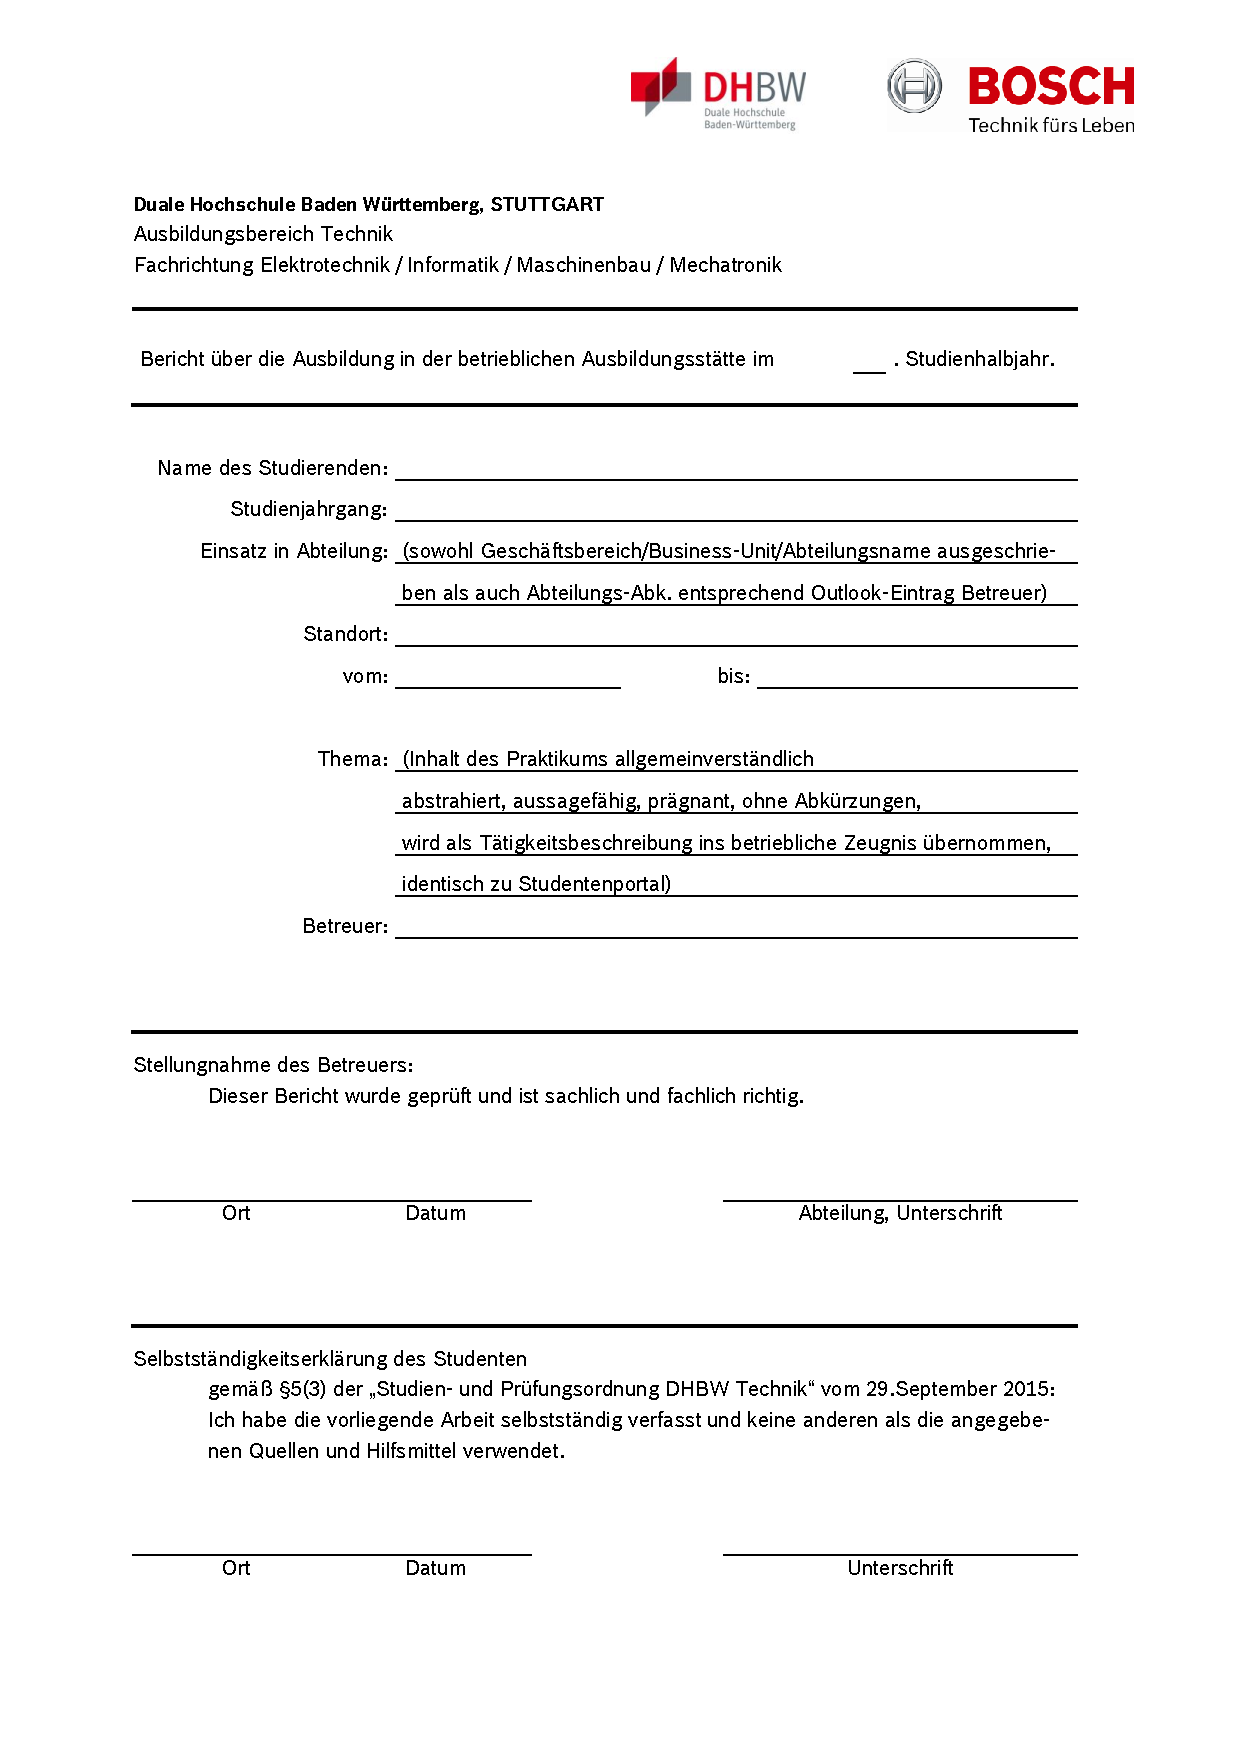
\includepdf[scale=1,clip,trim=0cm 1.5cm 0cm 2.5cm,pages={1},pagecommand={}]{ads/unterschriftenblatt}
        \newpage
    \fi

    % Selbstständigkeitserklärung nur einfügen, wenn Flag in den Einstellungen gesetzt ist
    \ifselbsterkl
        %!TEX root = ../dokumentation.tex

\thispagestyle{plain}
% Sperrvermerk direkt nach Selbstständigkeitserklärung
\section*{Selbstständigkeitserklärung}
%\section*{\\\langselbsterkl}

\vspace*{2em}


Wir versicheren hiermit, dass wir unsere {\arbeit} mit dem Thema: {\itshape{} \titel{}\/} selbstständig verfasst und keine anderen als die angegebenen Quellen und Hilfsmittel benutzt haben. Wir versicheren zudem, dass die eingereichte elektronische Fassung mit der gedruckten Fassung übereinstimmt.

\vspace{3em}

\abgabeort, \datumAbgabe
\vspace{4em}

\rule{6cm}{0.4pt}\\
\autor

        \newpage
    \fi

    % Sperrvermerk
    \ifsperrvermerk
        %!TEX root = ../dokumentation.tex

\thispagestyle{plain}
% Sperrvermerk direkt hinter Titelseite
\section*{\\\langsperrvermerk}

\vspace*{2em}

\iflang{de}{%
  Die vorliegende {\arbeit} mit dem Titel \begin{center}{\itshape{}\titel{}\/}\end{center}  enthält unternehmensinterne bzw. vertrauliche Informationen der {\firma}, ist deshalb mit einem Sperrvermerk versehen und wird ausschließlich zu Prüfungszwecken am Studiengang {\studiengang} der Dualen Hochschule Baden-Württemberg {\dhbw} vorgelegt. 
	\\
	\\
	Der Inhalt dieser Arbeit darf weder als Ganzes noch in Auszügen Personen außerhalb des Prüfungsprozesses und des Evaluationsverfahrens zugänglich gemacht werden, sofern keine anders lautende Genehmigung der Ausbildungsstätte ({\firma}) vorliegt.
}

%http://www.ib.dhbw-mannheim.de/fileadmin/ms/bwl-ib/Downloads_alt/Leitfaden_31.05.pdf

\iflang{en}{%
  The {\arbeit} on hand 
  \begin{center}{\itshape{} \titel{}\/}\end{center} 
   contains internal respective confidential data of {\firma}. It is intended solely for inspection by the assigned examiner, the head of the {\studiengang} department and, if necessary, the Audit Committee \langanderdh{} {\dhbw}. It is strictly forbidden:
    \begin{itemize}
    \item to distribute the content of this paper (including data, figures, tables, charts etc.) as a whole or in extracts,
    \item to make copies or transcripts of this paper or of parts of it,
    \item to display this paper or make it available in digital, electronic or virtual form.
    \end{itemize}
  Exceptional cases may be considered through permission granted in written form by the author and {\firma}.
}

\vspace{3em}

\abgabeort, \datumAbgabe
\vspace{4em}

\rule{6cm}{0.4pt}\\
\autor

        \newpage
    \fi

    % Abstract
    \ifabstract
        %!TEX root = ../dokumentation.tex


\newcommand{\deAbstractContent}{
    % deutschen Abstract hier einfügen!
    \todo{deutscher Abstract....}
}

\newcommand{\enAbstractContent}{
    % englischen Abstract hier einfügen!
    \todo{english abstract....}
}

%%%%%%%% Ab hier nicht mehr anfassen! %%%%%%%%

\newcommand{\deAbstract}{%
    \renewcommand{\abstractname}{\langabstract} % Text für Überschrift
    \begin{abstract}
        \thispagestyle{plain}
        \deAbstractContent
    \end{abstract}
}

\newcommand{\enAbstract}{
    \renewcommand{\abstractname}{\langabstract} % Text für Überschrift
    \begin{abstract}
        \thispagestyle{plain}
        \enAbstractContent
    \end{abstract}
}

\iflang{de}{
    \deAbstract
    \ifbothabstracts
        \clearpage
      %  \begin{otherlanguage}{english}
            \enAbstract
     %   \end{otherlanguage}
    \fi
}

\iflang{en}{
    \enAbstract
    \ifbothabstracts
        \clearpage
        \begin{otherlanguage}{ngerman}
            \deAbstract
        \end{otherlanguage}
    \fi
}
        \newpage
    \fi

    \pagestyle{plain}		% nur Seitenzahlen im Fuß

    %\RedeclareSectionCommand[beforeskip=\kapitelabstand]{chapter} 
    % Inhaltsverzeichnis
    \ifinhalt
        \begin{spacing}{1.1}
            \begingroup
                % auskommentieren für Seitenzahlen unter Inhaltsverzeichnis
                % \renewcommand*{\chapterpagestyle}{empty}
                % \pagestyle{plain}
                    
                    
                %\setcounter{tocdepth}{1}
                %für die Anzeige von Unterkapiteln im Inhaltsverzeichnis
                %\setcounter{tocdepth}{2}
                \pdfbookmark{\contentsname}{toc}
                \tableofcontents
                \clearpage
            \endgroup
        \end{spacing}
        \newpage
    \fi

    % Abkürzungsverzeichnis
    \ifabkverz
        \cleardoublepage
        \addchap{\langabkverz}

        \begin{acronym}[LOREMIPSUM] % Die Angabe in eckigen Klammern legt die Breite der linken Spalte fest! => ggf. anpassen
            \IfFileExists{{ads/sortedAcronyms}}{%		\ac{Abk.}   --> fügt die Abkürzung ein, beim ersten Aufruf wird zusätzlich automatisch die ausgeschriebene Version davor eingefügt bzw. in einer Fußnote (hierfür muss in header.tex \usepackage[printonlyused,footnote]{acronym} stehen) dargestellt
%		\acf{Abk.}   --> fügt die Abkürzung UND die Erklärung ein
%		\acl{Abk.}   --> fügt nur die Erklärung ein
%		\acp{Abk.}  --> gibt Plural aus (angefügtes 's'); das zusätzliche 'p' funktioniert auch bei obigen Befehlen
%		\acs{Abk.}   -->  fügt die Abkürzung ein
%	siehe auch: http://golatex.de/wiki/%5Cacronym
%!TEX root = ../dokumentation.tex
%nur verwendete Akronyme werden letztlich im Abkürzungsverzeichnis des Dokuments angezeigt
%Verwendung: 
\acro{BSP}{Board Support Package} % Beispielabkürzung
}{%!TEX root = ../dokumentation.tex
%nur verwendete Akronyme werden letztlich im Abkürzungsverzeichnis des Dokuments angezeigt
%Verwendung: 
%		\ac{Abk.}   --> fügt die Abkürzung ein, beim ersten Aufruf wird zusätzlich automatisch die ausgeschriebene Version davor eingefügt bzw. in einer Fußnote (hierfür muss in header.tex \usepackage[printonlyused,footnote]{acronym} stehen) dargestellt
%		\acs{Abk.}   -->  fügt die Abkürzung ein
%		\acf{Abk.}   --> fügt die Abkürzung UND die Erklärung ein
%		\acl{Abk.}   --> fügt nur die Erklärung ein
%		\acp{Abk.}  --> gibt Plural aus (angefügtes 's'); das zusätzliche 'p' funktioniert auch bei obigen Befehlen
%	siehe auch: http://golatex.de/wiki/%5Cacronym
\acro{BSP}{Board Support Package} % Beispielabkürzung

\acro{LIDAR}{Light Distance and Ranging}
\acro{ToF}	{Time of Flight}
\acro{3D}	{Dreidimensional}
\acro{CAD}	{Computer Aided Design}
\acro{NEMA}	{National Electrical Manufacturers Association}
\acro{GPIO}	{General Purpose Input Output}
\acro{APD}	{Avalanche Photo Diode}
\acro{SPAD}	{Single Photon Avalanche Diode}
\acro{UART} {Universal Asynchronous Reciever Transmitter}
\acro{I2C}	{Inter-Integrated Circuit}
\acro{SPI}	{Serial Peripheral Interface}
\acro{csv}	{comma separated values}
\acro{CNC}	{Computerized Numerical Control}	}
        \end{acronym}
    \fi

    % Abbildungsverzeichnis
    \ifabbverz
        \cleardoublepage
        \listoffigures
    \fi

    % Tabellenverzeichnis
    \iftableverz
        \cleardoublepage
        \listoftables
    \fi

    % Formelverzeichnis
    % mit "\formelentry{Formelname}" können neue Einträge erstellt werden. => auslagern in separates File? z.B. \input{ads/formels}
    \ifformelverz
        \cleardoublepage
        \listofformels
    \fi

    % Listingsverzeichnis
    \iflistverz
        \cleardoublepage
        \lstlistoflistings
    \fi

    \label{endOfRomanNumbering}

    \cleardoublepage

    %begin of new numbering
    \setpagestylecontent

    % Inhalt
    %!TEX root = ../dokumentation.tex

\chapter{Einleitung}
\todo{tbd..}
\section{lorem ipsum}
\subsection{merol muspi}
\Blindtext
\begin{equation}\formelentry{Beispielformel}
a = b + \lambda - \frac{\phi - \lambda}{2 \cdot \pi}
\end{equation} 
\subsection{ipsum lorem}
\blindtext

Ein Beispiel für die Verwendung eines Acronyms \ac{BSP}
mit Verweis auf eine Quelle \cite{Wollschlaeger2014}.

\begin{figure}[!htbp]
    \centering
    
\includegraphics[width=0.3\linewidth]{dhbw_de}
    \caption{DHBW-Logo}
    \label{fig:dhbw_logo}
\end{figure}

\section{Listings}
\subsection{lorem listum}

\begin{lstlisting}[caption={Einbinden von Code aus externer Datei mit Angabe eines Zeilenbereichs},label=inputFromFile]
\lstinputlisting[language=Python,firstline=37,lastline=45]{source_filename.py}
\end{lstlisting}

\blindmathpaper

\begin{lstlisting}[caption=Dies ist ein Listing,label=lstcode]
for i:=maxint to 0 do
begin
{ do nothing }
end;
Write('Case insensitive ');
Write('Pascal keywords.');
\end{lstlisting}

\begin{figure}[ht]%
	\centering
	\begin{circuitikz}
		\draw (0,0)
				to[V,v=$U_q$] (0,2)
				to[R=$R_1$] (2,2)
				to[short] (6,2)
				to[R=$R_2$] (6,0)
				to[short] (0,0);
	\end{circuitikz}
	\caption{Elektrische Schaltung - ein Beispiel}%
\end{figure}
%
    %!TEX root = ../dokumentation.tex
\chapter{Einleitung}\label{chap:einleitung}


Auf Baustellen und in der Innenarchitektur müssen ständig Räume vermessen werden. Herkömmliche Methoden, wie manuelle Laserentfernungsmesser sind teils ungenau und beanspruchen viel Zeit. Zudem werden dabei nur einzelne Raummaße ermittelt und 2D Grundrisse erstellt. Die für viele Planungsschritte notwendigen 3D Raumpläne werden aus Zeit- und Kostengründen nur selten erstellt. Dadurch ist die Bearbeitung ortsferner Projekte nur schwer oder gar nicht umsetzbar und häufig mit Planungsfehlern verbunden. \\
Geräte, die das Erstellen von 3D Raumkarten ermöglichen, sind sehr kostenintensiv und meist komplex in der Anwendung. Daher werden meist Dienstleistungsunternehmen benötigt, die die 3D Raumkarten erstellen. Die damit verbundenen enormen Kosten führen dazu, dass diese Methodik für kleine bis mittelgroße Bauprojekte nicht wirtschaftlich ist.

Im Rahmen dieser Studienarbeit soll ein System entstehen, welches das Erstellen von 3D Raumkarten ermöglicht. Ziel ist es, ein möglichst kostengünstiges und benutzerfreundliches Gerät zu entwickeln. Dieses soll in einem Raum aufgestellt werden und nach abgeschlossenem Messvorgang den Raum durch eine Punktewolke in 3D abbilden. Zusätzliche Anforderungen an das System sind eine hohe Genauigkeit und eine berührungslose Messung mittels eines \ac{LIDAR} Sensors.

Um genauere Anforderungen an das System definieren zu können, wird im Voraus ein Standardraum festgelegt. Angelehnt an einen größeren Raum in einem Gebäude, hat der Standardraum Abmaße von $5\:m$ x $6\:m$ x $3\:m$. Diesen Raum soll das System mit einer horizontalen Auflösung von 2 cm und einer vertikalen Auflösung von 5 cm abbilden können. Dies entspricht 1000 Messpunkten pro Quadratmeter und ca. 100000 Messpunkten im gesamten Raum. Dafür soll das System nicht länger als eine Stunde benötigen. 

Diese entstanden Punktewolke soll dazu dienen, ortsferne Planung zu erleichtern. In dem 3D Modell des Raums können beliebige Maße direkt abgelesen werden. Das Modell ist drehbar, stellt komplexe Konturen dar und ermöglicht jegliche Ansicht.
Die 3D-Modellierung kann durch die frei wählbare Ansichten zusätzlich für virtuelle Immobilienpräsentationen und weitere Animationen verwendet werden.      


Der erste Teil dieser Studienarbeit beschäftigt sich mit den Grundlagen der Laserentfernungsmessung. Im Anschluss daran folgt eine Machbarkeitsstudie, einen \ac{LIDAR} Sensor mittels kostengünstiger Komponenten selbst zu entwerfen und zu bauen. Das Resultat dieser Machbarkeitsstudie bestimmt den verwendeten Sensor für das Projekt. Ist ein kostengünstiger Selbstbau eines Sensors möglich, der den Anforderungen entspricht, wird dieser verwendet. Ist dies nicht möglich, werden passende Sensoren ausgewählt und zugekauft. Der direkte Vergleich der Sensoren erfolgt mit dem fertigen System.\\
Der Hauptteil der Arbeit beschäftigt sich mit der Konzipierung, dem Bau und den Tests des eigentlichen Systems. Während der Konzipierung und des Baus wird das Projekt in drei Kategorien aufgeteilt.\\
Der erste Teil ist die Mechanik, welche den Sensor in zwei Achsen drehen kann um einen kompletten dreidimensionalen Raum abtasten zu können. Der zweite Teil beschäftigt sich mit den elektronischen Komponenten und deren Verbindungen untereinander. Der dritte Teil beschäftigt sich mit der Programmierung sowohl der Ansteuerung der Komponenten aus Teil zwei, als auch der Auswertung und Visualisierung der Daten.

Im Anschluss daran wird das System getestet und verschiedene Auflösungen, Darstellungsarten und Sensoren verglichen.
%
    %!TEX root = ../dokumentation.tex
\chapter{Grundlagen Elektronik}\label{chapter:grundlagenet}
\section{Photodioden}\label{sec:photodioden}
Um Licht zu detektieren werden meist Photodioden verwendet. Diese arbeiten nach einem relativ einfachen Prinzip.
Eine p-n-Diode wird in Sperrrichtung betrieben, durch die Angelegte Spannung entsteht eine Sperrschicht. Wenn nun Photonen auf die offene, starke p-Dotierung treffen werden dort durch den Photoeffekt Ladungsträger erzeugt (Abbildung: \ref{photodiode}). Wenn diese nun durch Diffusion bis zur Sperrschicht gelangen, driften die Ladungsträger entgegen der Sperrspannung in die jeweiligen Raumladungszonen, dies ist als Strom messbar. \cite{Photodiode_spektrum}
\begin{figure}[H]
	\centering
	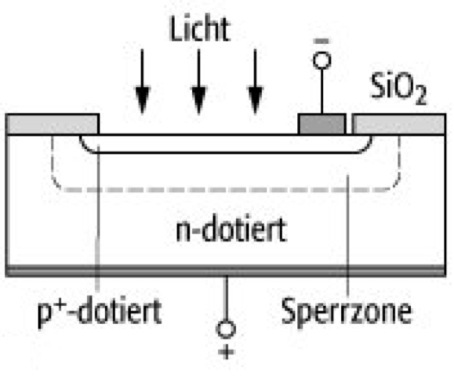
\includegraphics[width=0.75\textwidth]{images/GrundlagenLaserentfernungsmessung/Photodiode}
	\caption{Schematischer Aufbau einer Photodiode \cite{Photodiode_spektrum} ($p^+$ starke p-Dotierung)}
	\label{photodiode}
\end{figure}
Dieser Effekt tritt allerdings nur auf, wenn die Photonen eine Energie großer als die des Bandabstandes des verwendeten Halbleiters aufweisen. Hierbei ist zudem pro eintreffendem Photon nur ein sehr geringer Stromimpuls messbar, daher ist diese Art von Diode für \ac{LIDAR} Anwendungen nicht brauchbar.
\subsection{\acf{APD}}\label{subsec:apd}
Um einzelne Photonen detektieren zu können wird eine spezielle Form der Photodiode verwendet. Die sogenannte \ac{APD}. Die \ac{APD} hat im Gegensatz zur herkömmlichen Photodiode zweit weitere Schichten. Hinzu zur n-Dotierten und stark p-Dotierten Schicht kommen nun eine schwach p-Dotierte (oder intrinsische) und eine "normal" p-Dotierte Schicht (Abbildung: \ref{apd}). 
\begin{figure}[H]
	\centering
	
\includegraphics[width=0.75\textwidth]{images/GrundlagenLaserentfernungsmessung/APD}
	\caption{Schematischer Aufbau einer \ac{APD} \cite{APD_Scematic} ($p^+$ starke p-Dotierung, $p^- (\pi)$ schwache (intrinsische) p-Dotierung, $n^+$ starke n-Dotierung) (1 - Metallkontakte, 2 - Entspiegelung)}
	\label{apd}
\end{figure}
Wenn Photonen nun in die $\pi$ Zone gelangen, werden dort Landungsträger erzeugt, diese werden gleich wie bei der regulären Photodiode getrennt, Löcher wandern Richtung $p^+$-Zone und Elektronen Richtung $n^+$-Zone. Durch die stärker Dotierte p-Zone, und somit höhere Feldstärke, werden die Elektronen beschleunigt und es entsteht eine Stoßionisation. \ac{APD} werden mit sehr hohen Sperrspannungen $\sim$100V, nahe der Durchbruchspannung betrieben. \cite{SPAD_mamamatsu} \\
Wenn die \ac{APD} oberhalb der Durchbruchsspannung betrieben wird, setzt sich die Stoßionisation lawinenartig fort (Avalanche-Effekt) und es entstehen Verstärkungsfaktoren von einigen Millionen. \ac{APD} welche speziell für den Betrieb oberhalb der Durchbruchspannung ausgelegt sind werden auch \ac{SPAD} genannt. Mittels diesem Effekt kann man einzelne Photonen nachweisen, da jedes Photon einen kurzen detektierbaren Stromimpuls erzeugt. Bei der anordnung vieler solcher \acp{SPAD} in einem Array können viele einzelne Photonen präzise nachgewiesen werden. \cite{SPAD_elmer}\\
\subsection{Lateral auflösende Photodiode}
Die lateral auflösende Photodiode, auch \ac{PSD} genannt, verwendet mehrere aneinander geschlossene Photodioden zur Bestimmung der Position eines Lichtpunktes.
\begin{figure}[H]
	\centering
	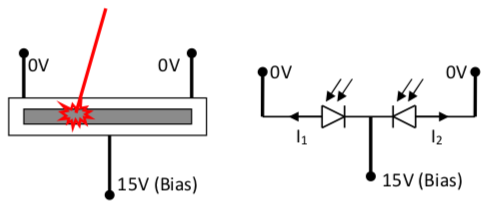
\includegraphics[width=0.75\textwidth]{images/GrundlagenLaserentfernungsmessung/PSD}
	\caption{Aufbau einer \ac{PSD} \cite{APD_Scematic}}
\end{figure}
Wenn man nun jeweils den Photostrom der Dioden miteinander Vergleicht kann man eine sehr präzise Auskunft über die Position des Lichtpunkts geben.
\begin{equation}\formelentry{Position des Lichtpunkts einer \ac{PSD}}
	x = \frac{I_1 - I_2}{I_1 + I_2}
\end{equation}
\begin{flalign*}
	&I_1 = \text{Strom aus der linken Photodiode}\left[A \right]&\\
	&I_2 = \text{Strom aus der rechten Photodiode} \left[A \right]&\\
	&x = \text{Relative Position des Lichtpunktes}&
\end{flalign*}
Die Differenz der Ströme wird hier auf den Gesamtstrom Normiert, dies hat zur Folge, dass die Position unabhängig von der Intensität des Lichts wird.\\
Um diese Auswertung zu realisieren ist lediglich eine Transimpedanzverstärkerschaltung gekoppelt mit einer Komperatorschaltung nötig, mit welcher die Spannungen verglichen werden können.\\
Ein sehr großer Vorteil der \ac{PSD} gegenüber anderer Methoden zur Feststellung der Position eines Lichtpunkts ist, dass die \ac{PSD} innerhalb von Nanosekunden reagieren und das mit einer Sehr genauen Auflösung.\cite{psd}

%Marcel
    %!TEX root = ../dokumentation.tex
\chapter{Grundlagen Laserentferungsmessung}\label{sec:grund_lidar}
Um eine Entfernung zu einem Punkt mittels Licht zu bestimmen gibt es verschiedene Möglichkeiten, welche im folgenden Kapitel näher behandelt werden. Ein wichtiger Hinweiß ist zudem, dass im Zusammenhang mit dem Thema \ac{LIDAR} oftmals der Begriff '\acf{ToF}' fällt, dieser beschreibt allerdings nicht immer das direkt damit verbundene Verfahren, sondern allgemein die Entfernungsbestimmung mittels Licht. 
\section{Lichtlaufzeitmessung}
\subsection{Grundprinzip}
Das Grundprinzip der Lichtlaufzeitmessung oder auch \acf{ToF} (Abbildung: \ref{tof}), bezieht sich auf die Zeit, welche ein ausgesandter Lichtimpuls benötigt bis er wieder am Sender eintrifft.\\
\begin{figure}[H]
	\centering
	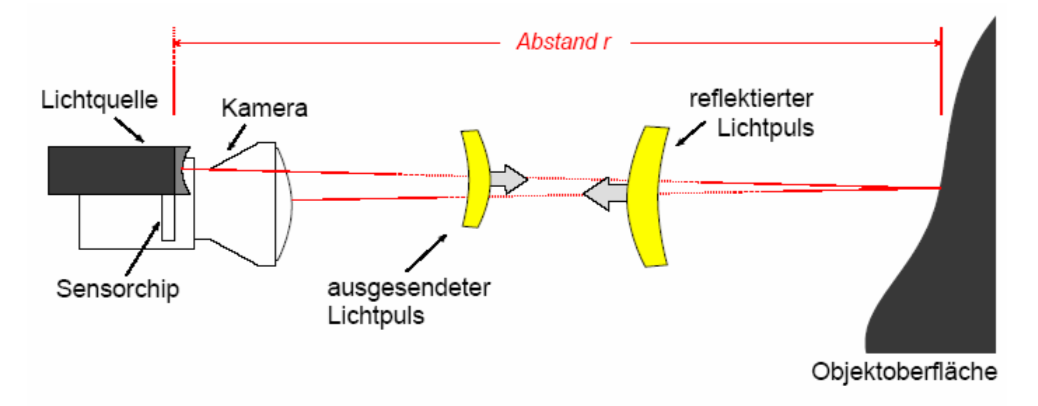
\includegraphics[width=0.75\textwidth]{images/GrundlagenLaserentfernungsmessung/ToF}
	\caption{\ac{ToF} Prinzip \cite{ToF_TUBerlin}}
	\label{tof}
\end{figure}
Dazu wird ein einzelner kurzer Lichtpult von der Lichtquelle ausgesandt, welcher dann von der Oberfläche reflektiert wird und anschließend von einem Sensorchip wieder detektiert werden kann. Über die Zeitdifferenz zwischen aussenden und detektieren des Lichtimpulses und die (halbe) Lichtgeschwindigkeit kann anschließend auf die Entfernung des getroffenen Punktes geschlossen werden. \cite{ToF_ST}
\begin{equation}\formelentry{Berechnung der Entfernung mittels Lichtlaufzeit}\label{lichtlaufzeit}
	r = \frac{t_{diff}}{2} \cdot c
\end{equation} 
\begin{flalign*}
	&r = \text{Abstand zum getroffenen Punkt } \left[m \right]&\\
	&t_{diff} = \text{Zeitdifferenz zwischen aussenden und detektieren des Lichtpulses}\left[s \right]&\\
	&c = \text{Lichtgeschwindigkeit in Luft}\left[\frac{m}{s} \right]&
\end{flalign*}
Ein großer Vorteil des \ac{ToF} Verfahrens ist, dass durch die Reflexion von Partikeln in der Luft beispielsweiße auf die Luftqualität oder die Luftfeuchtigkeit geschlossen werden kann. Dies macht sich am Sensor als vor der größten Reflexion (Oberfläche) auftretende kleine Reflexion bemerkbar.
\subsection{Herausvorderungen}\label{subsec:tof_herausvorderungen}
Bei dieser Technologie entstehen allerdings einige Probleme, auf welche im Folgenden eingegangen wird. Generell sind alle Probleme welche bei \ac{ToF} auftreten miteinander verknüpft, bzw. bedingen sich gegenseitig. \\
Das erste Problem welches Auftritt ist, dass nie das gesamte ausgesandte Licht zur Detektion zur verfügung steht. Durch verschiedene Reflexionsgrade verschiedener Oberflächen und die generelle Streuung des Lichts bei auftreffen auf eine Oberfläche wir immer nur ein geringer Teil direkt zum Sensor zurückgeworfen. Daher sind hoch empfindliche Sensoren nötig um eine zuverlässige Detektion zu ermöglichen.
\ac{SPAD} sind für die Anwendung in einem \ac{ToF} \ac{LIDAR} System sehr gut geeignet, vor allem in einer Anordnung zu einem Array, da eine größere Sensorfläche mit gleichbleibender Genauigkeit realisiert werden kann, und somit eine größere Streuung des reflektierten Lichts abgedeckt werden kann. Allerdings ist das Detektieren des zurückgeworfenen Lichts nicht die einzige Herausforderung welche auftritt, denn mit steigender Distanz nimmt die Dämpfung des Lichtimpulses immer weiter ab. Eine Lösung dafür könnte sein eine Stärkere Lichtquelle zu verwenden, dies birgt allerdings große Sicherheitsrisiken und ist daher nur begrenzt möglich. Eine zweite Lösung ist, die maximale Messentfernung zu limitieren, allerdings birgt dies ein anderes Problem dieses und ein weiteres Problem, welches im Zusammenhang mit der minimalen Messentfernung steht, wird anhand eines Beispiels erläutert.\\
Man nehme an, es existiert ein fiktiver \ac{LIDAR} Sensor mit folgenden Werten:
\begin{itemize}
	\item Minimale Messentfernung $d_{min}=1cm$
	\item Maximale Messentfernung $d_{max}=1000m$
	\item Maximale Messfrequenz $f_{max}=150kHz$ 
\end{itemize}
Formel \ref{lichtlaufzeit} kann umgestellt werden, um die Zeiten zu errechnen, welche das Licht für die minimale und maximale Messentfernung benötigt. 
\begin{equation}\formelentry{Berechnung der minimalen und maximalen Zeit}
	\begin{split}
		t = \frac{r \cdot 2}{c}\\
		t_{min} = \frac{0.01 \cdot 2}{299,79 \cdot 10^6} = 667,13 \cdot 10^{-9}\\
		t_{max} = \frac{1000 \cdot 2}{299,79 \cdot 10^6} = 6,6713 \cdot 10^{-6}\\
	\end{split}
\end{equation} 
\begin{flalign*}
	&r = \text{Abstand zum getroffenen Punkt } \left[m \right]&\\
	&t = \text{Zeitdifferenz zwischen aussenden und detektieren des Lichtpulses}\left[s \right]&\\
	&c = \text{Lichtgeschwindigkeit in Luft}\left[\frac{m}{s} \right]&
\end{flalign*}
Anhand des Beispiels kann man bereits erkennen, dass um die gewünschte minimale Messentfernung zu realisieren eine extrem schnelle Schaltung nötig ist, um das Aussenden und Empfangen innerhalb von $667,13ns$ zu detektieren. Die maximale Messentfernung bringt in diesem Fall ein anderes Problem mit sich, welches noch nicht erwähnt wurde. Zwar ist dies nur ein fiktives Beispiel, allerdings muss das Problem trotzdem betrachtet werden. Der Sensor ist mit einer Maximalen Frequenz von $150kHz \rightarrow 6,6667\mu s$ angegeben, allerdings kann mit dieser Frequenz die maximale Messentfernung nicht erreicht werden, da das Licht länger benötigt. \\
Durch dieses Beispiel wurde veranschaulicht, dass verschiedene Faktoren die Grenzen des Sensors festlegen. Die minimale Messentfernung wird definiert dadurch, wie schnell die Schaltung Aussenden und Empfangen detektieren kann. Die maximale Messentfernung wird von Leistung der Lichtquelle sowie Genauigkeit des Sensors definiert. Die maximale Messfrequenz hängt zusätzlich noch davon ab, wie schnell der Sensor die Daten zur Weiterverarbeitung z.B. an einer \ac{UART} Schnittstelle bereitstellen  kann.

\section{Phasenverschiebung / Phasenmodulation}  \label{sec:phasenverschiebung}
Das Phasenverschiebungsverfahren macht sich zu nutzen, dass bei einer ausgesandten Elektromagnetischen Welle die Phase immer größer wird bei steigender Entfernung. Durch Aussenden verschieden Frequentierter Wellen kann dann die Phasenverschiebung der Wellen bestimmt werden und daraus die Entfernung\cite{phasenverschiebung}.\\
\subsection{Grundprinzip}
Das Grundprinzip des Phasenverschiebungsverfahren basiert auf der Inferometrie.\\
Die Inferometrie besagt lediglich, dass die Messergebnisse auf der Interferenz, also der Überlagerung mehrerer Wellen, beruht. Interferenzen treten bei verschiedensten Formen von Wellen auf, nicht nur bei Elektromagnetischen Wellen, sondern auch bei z.B. mechanischen Wellen wie Schall- oder Wasserwellen\cite{inferometrie}.\\
\begin{figure}[H]
	\centering
	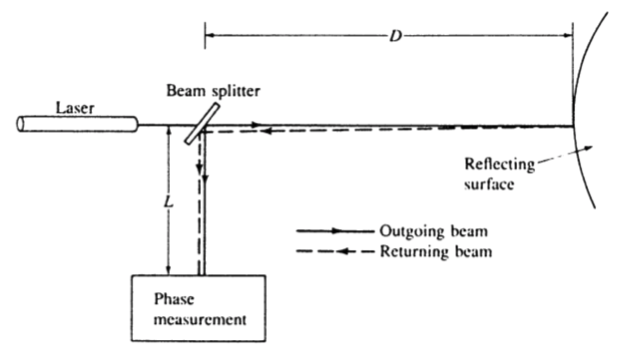
\includegraphics[width=0.75\textwidth]{images/GrundlagenLaserentfernungsmessung/Phasenverschiebung}
	\caption{Versuchsaufbau Phasenverschiebungsentfernungsmessung \cite{lichtabstandsmessung}}
	\label{phasenverschiebung}
\end{figure}
Bei einem Versuchsaufbau nach dem Prinzip in Abbildung \ref{phasenverschiebung}, wird der vom Laser ausgesandte Lichtstrahl zuerst aufgeteilt, damit dieser dann als Referenzwert zur Bestimmung der Phasendifferenz verwendet werden kann. Der zweite Pfad des Lichtstrahls wird sich weiter in Richtung der Oberfläche bewegen, bis dieser schließlich von der Oberfläche reflektiert wird und durch einen Umlenkspiegel ebenfalls zur Bestimmung der Phasendifferenz verwendet wird.\\
Wenn die Distanz $D=0$ ist, kommen die beiden Lichtstrahlen gleichzeitig bei der Phasenbestimmung an. Bei einer Entfernung ungleich 0 ist die zurückgelegte Strecke des Lichtstrahls.
\begin{equation}\formelentry{Zurückgelegte Strecke des Lichtstrahls}
	E = L + 2 \cdot D
\end{equation} 
\begin{flalign*}
	&E = \text{Zurückgelegte Strecke des Lichtstrahls} \left[m \right]&\\
	&L = \text{Abstand zwischen Spiegel und Phasenbestimmung}\left[m \right]&\\
	&D = \text{Abstand zwischen Spiegel und Oberfläche}\left[m \right]&
\end{flalign*} 
Da wie bereits erwähnt die Phase mit steigender Entfernung größer wird kann von dieser Phasenänderung auf die Wellenlänge geschlossen werden. 
\begin{figure}[H]
	\centering
	\includegraphics[width=0.75\textwidth]{images/GrundlagenLaserentfernungsmessung/phase}
	\caption{Phasendifferenz einer Welle \cite{frauenhoferipm}}
	\label{phasendifferenz}
\end{figure}
Die Phase kann als ein Vielfaches der Wellenlänge $\lambda = \frac{c}{f}$ und somit als Entfernung ausgedrückt werden. 
\begin{equation}\formelentry{Zurückgelegte Strecke des Lichtstrahls}\label{streckephase}
	\begin{split}
		\varphi = \frac{4\cdot\pi \cdot D}{\lambda}\\
		D = \frac{c\cdot\varphi}{4\cdot\pi\cdot f_{m}}
	\end{split}
\end{equation} 
\begin{flalign*}
	&D = \text{Abstand zwischen Laser und Oberfläche}\left[m \right]&\\
	&\varphi = \text{Phasendifferenz} \left[^{\circ} \right]&\\
	&\lambda = \text{Wellenlänge}\left[m \right]&\\
	&f_{m} = \text{Modulationsfrequenz} \left[\frac{1}{s} \right]&\\
	&c = \text{Lichtgeschwindigkeit} \left[\frac{m}{s} \right]&
\end{flalign*}
Allerdings bringt die Verwendung nur einer Wellenlänge zur Modulation des Lasers zur Bestimmung der Phasendifferenz einige Probleme mit sich. Zum einen wird die Gleichung \ref{streckephase} bei jedem Vielfachen $n$ von $360^{\circ}$ die gleiche Lösung ergeben, somit kann man die Distanz nicht eindeutig bestimmen. Zum anderen ist der Aufbau wie in \ref{phasenverschiebung} nur für wenige Anwendungen geeignet, daher wurde in Abbilding \ref{phasendifferenz} bereits ein anderer besser nutzbarer Aufbau gezeigt. \\
Das Problem der uneindeutigkeit kann gelöst werden, indem man den Lichtstrahl kontinuierlich mit mehreren Signalen mit unterschiedlichen Frequenzen moduliert wird. Anschließend wird für jede der ausgesandten Frequenzen die Phasendifferenz bestimmt. Dies bringt den großen Vorteil, dass durch Überlagerung der Ergebnisse eine Eindeutigkeit festgestellt werden kann und sich die Messgenauigkeit somit deutlich erhöht\cite{lichtabstandsmessung}\cite{phasenmodulation}\cite{frauenhofer}.\\
Einige der Vorteile, welche beim Phasenverschiebungsverfahren bestehen sind, dass die Bauteile um ein vielfaches langsamer sein können, als beim \ac{ToF} Verfahren. Dies ist darauf zurückzuführen, dass es prinzipiell egal ist bei welchem Nulldurchgang einer Welle die Phase bestimmt wird, da sich nur ein vielfaches von $360^{\circ}$ zur Phase addiert wird. Durch Verwendung mehrerer Modulationsfrequenzen kann trotzdem eine Eindeutigkeit gewährleistet werden.\\
Dazu kommt auch, dass mit Modulationsfrequenzen im Megaherz Bereich sehr hohe Messgenauigkeiten möglich sind, da diese von der hochsten Modulationsfrequenz abhängt.
\begin{equation}\formelentry{Beispielrechnung Messgenauigkeit}\label{streckephase}
	\lambda = \frac{c}{f_{m}} = \frac{c}{150\cdot 10^{6}} \approx 2
\end{equation} 
\begin{flalign*}
	&\lambda = \text{Wellenlänge}\left[m \right]&\\
	&f_{m} = \text{Modulationsfrequenz} \left[\frac{1}{s} \right]&\\
	&c = \text{Lichtgeschwindigkeit} \left[\frac{m}{s} \right]&
\end{flalign*}
Bei einer Wellenlänge von $2m$ liegt der eindeutige Bereich zwar nur noch bei einem Meter, jedoch lässt sich die Phasendifferenz sehr genau bestimmen und somit ist eine höhere Genauigkeit möglich als besipielsweiße bei einer Wellenlänge von $150m$.
\subsection{Herausforderungen}
Eine der größten Herausforderungen des Phasenverschiebungsverfahrens sind Störeinflüsse aus der Umwelt. Regen beispielsweiße kann sich sehr störend auf die Messergebnisse auswirken. Ebenfalls kann keine Zusätzliche information aus der Reflexion erlangt werden, wie dies beispielsweiße beim \ac{ToF} Verfahren möglich ist.\\
Die zum \ac{ToF} Verfahren vergleichsweise wenigen Herausforderungen sind Grund dafür, dass das Phasenverschiebungsverfahren sehr weit verbreitet ist und in viele Anwendungen findet.
\section{Triangulation}
Beim Triangulationsverfahren wird sich wie der Name schon vermuten lässt die Trigonometrie zu nutzen gemacht.\\

\subsection{Grundprinzip}
Wenn bei einem Dreieck zwei Punkte, deren Distanz zueinander und der Winkel zum Dritten Punkt bekannt ist, dann auch die Position des dritten Punktes bestimmt werden (Abbildung \ref{triangulation}).
\begin{figure}[H]
	\centering
	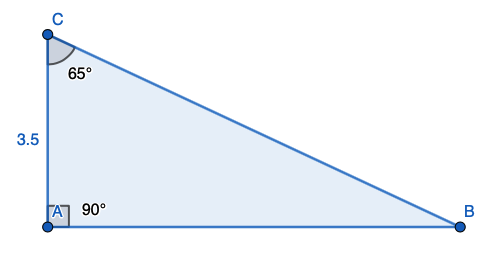
\includegraphics[width=0.75\textwidth]{images/GrundlagenLaserentfernungsmessung/Triangulation}
	\caption{Beispiel Triangulation}
	\label{triangulation}
\end{figure}
Nun kann durch Anwendung bekannter Trigonometrischer Funktionen die Position des dritten Punktes, und damit die Entfernung, bestimmt werden.
\begin{equation}\formelentry{Sinussatz}\label{trigonometrie}
	\frac{c}{sin(\gamma)} = \frac{b}{sin(\beta)} = \frac{a}{sin(\alpha)} 
\end{equation}
\begin{flalign*}
	&a = \text{Stecke BC}\left[m \right]&\\
	&b = \text{Strecke AC} \left[m \right]&\\
	&c = \text{Strecke AB} \left[m \right]&\\
	&\alpha = \text{Winkel an A} \left[^{\circ} \right]&\\
	&\beta = \text{Winkel an B} \left[^{\circ} \right]&\\
	&\gamma = \text{Winkel an C} \left[^{\circ} \right]&
\end{flalign*}
Für das gegebene Beispiel wäre dies:
\begin{equation}\formelentry{Beispielrechnung Trigonometrie}\label{bsp_trigonometrie}
	\begin{split}
		\beta = 180^{\circ} - \alpha - \gamma = 25^{\circ}\\
		c = \frac{b\cdot sin(\gamma)}{sin(\beta)} = 7.5\\
		a = \frac{b\cdot sin(\alpha)}{sin(\beta)} = 8.28
	\end{split}
\end{equation}
Da die Winkel bekannt sind ist nun bekannt, dass der Punkt B an $x = 7.5$ und $y = 0$ liegt. Somit wurde die Entfernung bestimmt.\\
Der Aufbau wie in Abbildung \ref{triangulation} kann auch mit Sender und Empfänger realisiert werden. Dazu wird angenommen, dass in Punkt A ein Sender, also Laser oder LED (nur für geringe Anforderungen) positioniert wird. In Punkt C wird ein \ac{PSD} positioniert.\\
Wenn man nun eine Bikonvexe Linse vor das \ac{PSD} positioniert wir das gesamte einfallende Licht gebündelt und als ein Punkt auf dem \ac{PSD} messbar.
Durch den Abstand des \ac{PSD} zur Linse und die Position des Lichtpunkts auf dem \ac{PSD} lässt sich dann der Winkel des einfallendes Lichts bestimmen.\\
Dieser Winkel kann dann wie beschrieben zur Bestimmung der Entfernung der reflektierenden Oberfläche verwendet werden. \\
Ein sehr großer Vorteil des Triangulationsverfahrens ist, dass es mit sehr preiswerten Bauteilen realisiert werden kann, da wie bereits erwähnt für Anwendungen mit sehr niedrigen Anforderungen eine \ac{LED} als Lichtquelle ausreicht. Ebenfalls sind die Photodioden nicht kompliziert oder teuer, anders als beispielsweiße \ac{SPAD} Dioden welche für \ac{ToF} oder Phasenverschiebung Verfahren verwendet werden.\\
Zudem kann durch konstantes einschalten der Lichtquelle sehr gut eine Geschwindigkeit bestimmt werden, da die \ac{PSD} innerhalb von wenigen Nanosekunden ihren Strom ändern und somit eine sehr schnelle detektion eines sich bewegenden Objekts möglich ist. \cite{triangulation}\cite{psd}
\subsection{Herausforderungen}
Durch Störeinflüssen wie beispielsweiße anderes einfallendes Licht kann die Messung stark beeinflusst werden. Ebenfalls kann es gerade durch die Verwendung von preiswerten Bauteilen zu großen Toleranzen kommen wodurch die Messergebnisse stark schwanken können. Auch kann ähnlich wie beim Phasenverschiebungsverfahren keine Auskunft über weitere Parameter gegeben werden. %Marcel
    %!TEX root = ../dokumentation.tex


\chapter{Grundlagen}

\section{Schrittmotoren}

Beim Schrittmotor handelt es sich um einen Synchronmotor. Innerhalb des feststehenden Strators befindet sich ein drehend gelagerter Rotor. Wird ein Schrittmotor entsprechend angesteuert, dreht sich der Rotor um einen bestimmten Drehwinkel weiter. Durch mehrere Schritte kann der Rotor um jeden Drehwinkel, der einem Vielfachen des minimalen Drehwinkels entspricht, gedreht werden. \\
Man unterscheidet drei Bauformen von Schrittmotoren: \\
Der Reluktanz-Schrittmotor ist die älteste Bauweise von Schrittmotoren. Dabei besteht der gezahnte Rotor sowie der Strator aus weichmagnetischen Material. Durch Anlegen von Strömen bilden sich magnetische Felder aus und der Rotor dreht sich. Durch die fehlenden Permanentmagneten hat der Motor jedoch kein Rastermoment im ausgeschalteten Zustand.\\
Beim Permanentmagnet-Schrittmotor besteht der Strator aus Weicheisen und der Rotor aus Permanentmagneten. Durch geschickte Bestromung des Strators, wird der Rotor immer so ausgerichtet, dass eine Drehbewegung entsteht. In dieser Bauform ist die Auflösung durch die limitierte Anzahl von Polen begrenzt.\\

Beim Hybridschrittmotor werden die Vorzüge der beiden genannten Motorarten vereint. Der Strator besteht aus gezahntem Weichmetall. Der Rotor besteht aus einem Permanentmagneten mit axialer Magnetfeldausrichtung. Darauf werden zwei fein gezackte, weichmagnetische Dynamobleche angebracht. Diese sind zueinander verdreht, sodass es zu einer Polteilung kommt und sich Süd- und Nordpole abwechseln. Der Hybridmotor zeichnet sich durch gutes Drehmoment und eine gute Auflösung aus.

--ToDO: Quellen und Bilder einfügen, allgemeine Funktion beschreiben --%Alexander
    %!TEX root = ../dokumentation.tex
\chapter{Stand der Technik}\label{chap:stand_der_technik}
\todo{Meeeehr Text}\\
Im folgenden Kapitel sollen bereits vorhandene \ac{LIDAR} Systeme betrachtet werden.\\
Dabei wird ein vergleich verschiedener Systeme, sowie die Analyse deren Funktionen und die mögliche Übertragung dieser Funktionen auf das in dieser Arbeit entstehende System erfolgen.\\
Die Systeme, welche Verglichen werden, sind meist für die Anwendung im Bereich der Geodäsie entwickelt, und ermöglichen ein schnelles Präzises dreidimensionales vermessen von Landschaften oder Baustellen. Zusätzlich werden auch Systeme welche für Logistik oder Raumvermessung entwickelt worden sind verglichen. \\

\section{Vergleich der Sensoren}
Bei Betrachtung der Tabelle \ref{vergleich_sensoren} kann beobachtet werden, dass je nach Anwendungsgebiet des Sensors unterschiedliche Parameter Ausschlag gebend für den Entwurf des Systems sind. Zudem kann betrachtet werden, dass Systeme in dieser Kategorie sehr Preisintensiv sind. \\
Vor allem sticht die maximale Messrate der Verschiedenen Sensoren besonders hervor und ist dabei stark vom Einsatzgebiet abhängig. Gerade bei Systemen, welche für den Außenraum konzipiert sind, ist eine hohe Messrate gefordert, damit in einer annehmbaren Zeit ein möglichst genaues Abbild der Umgebung erstellt werden kann. Auch ist eine große Reichweite von Vorteil, damit auch Objekte in großer Entfernung noch Aufgezeichnet werden können. \\
Zudem kann beobachtet werden, dass die meisten der Systeme das \ac{ToF} Prinzip verwenden. Dadurch werden zum einen hohe Messfrequenzen möglich, zum anderen lassen sich auch Zusatzfunktionen wie z.B. die Multi-Echo Auswertung implementieren. \\
Die großen Unterschiede der Auflösung sind ebenfalls auf die Anforderungen aus den verschiedenen Anwendungsgebieten zurückzuführen. Da beim Vermessen von Gebäuden oder Landschaften eine hohe Auflösung gerade für die Planung sehr wichtig ist. Bei der Logistik kommt es allerdings eher auf einen geringen Preis an, als eine Millimeter genaue Auflösung, da ohnehin immer ein Abstand zum Hindernis gewahrt werden muss.\\
Die große Preisspanne der Verschiedenen Systeme ist den verschiedenen Anwendungsgebieten geschuldet, da die Sensoren dort unterschiedlich oft eingesetzt werden. So müssen für die Automatisierung einer Logistikzentrale beispielsweise viele der Systeme verbaut werden, während für das Erfassen der Außenumgebung ein ein einzelnes System vollkommen ausreichend ist.

\begin{landscape}
	\begin{table}[H]
		\centering
		\caption{Vergleich verschiedener \ac{3D} \ac{LIDAR} Systeme}\label{vergleich_sensoren}
		\begin{tabular}{|c|c|c|c|c|}
			\hline
			& \textbf{Sick MRS6000 \cite{sick}} & \textbf{\begin{tabular}{@{}c@{}}Ocular\\Robotics RE05\end{tabular} \cite{ocular}} & \textbf{\begin{tabular}{@{}c@{}}Leica Scan\\Station P50\end{tabular} \cite{leica}} & \textbf{Artec Ray \cite{artec}}\\
			\hline
			\textbf{Anwendungsgebiet} & Logistik & Innenraum & Außenraum & Außenraum \\
			\hline
			\textbf{Reichweite [m]} &  200 & 160 & >1000 & 110   \\
			\hline
			\textbf{Messrate [Hz]} &  10 & 30000 & 1000000 & 208000   \\
			\hline
			\textbf{Auflösung [mm]} & 125 & 50 & 3 & 0.9   \\
			\hline
			\textbf{Verfahren} &  
				\begin{tabular}{@{}c@{}} 
					\ac{ToF} \& \\ Bewegende Polygonspiegel 
				\end{tabular} &  
				- &  
				\begin{tabular}{@{}c@{}} 
					\ac{ToF} \& \\
					Rotierender \\ 
					Sender/Empfänger
				\end{tabular} & 
				\begin{tabular}{@{}c@{}} 
					Phasenverschiebung \& \\ 
					Rotierender \\
					Sender/Empfänger
				\end{tabular} 
				 \\
			\hline
			\textbf{Zusatzfunktionen} & 
				\begin{tabular}{@{}c@{}} 
					Multi-Echo \\
					Auswertung
				\end{tabular} &
				\begin{tabular}{@{}c@{}} 
					Horizontales einstellen \\ des Messbereichs
				\end{tabular} &  
				\begin{tabular}{@{}c@{}} 
					Farbkamera \\
					
				\end{tabular} &  
				
			\\
			\hline
			\textbf{Preis [Euro]} & 7000 & - & 125500 & 50000
			\\\hline
		\end{tabular}
	\end{table}
\end{landscape}

\section{Erkenntnisse}
Die größte Erkenntnis aus den Ergebnissen des Vergleichs ist, dass man immer Kompromisse bei der Auslegung eines Systems eingehen muss. Vor allem ist der Kostenpunkt der größte Limitierende Faktor, da dieser vorgibt, welche Methode verwendet wird und welche Messraten möglich wird. 
\todo{Nichts für innenraum, nur als dienstleistung oft möglich, sehr teuer, kompromisse nötig}
%
    %!TEX root = ../dokumentation.tex
\chapter{Machbarkeitsstudie}\label{chap:machbarkeitsstudie}
Ziel der Machbarkeitsstudie ist es, Informationen über die Schwierigkeit des Entwurfs und der Herstellung eines \ac{LIDAR} Sensors mittels einer Photodiode zu erlangen. 

\section{Versuch 1: Test handelsüblicher Photodioden}
In einem ersten sehr einfachen Aufbau wurde der Photostrom in einer Handelsüblichen Photodiode gemessen.
\subsection{Versuchsaufbau}
\subsubsection{Verwendete Bauteile}

\begin{table}[H]
	\centering
	\caption{Bauteilliste Versuch 1}
	\begin{tabular}{|l|l|}
		\hline
		\textbf{Bezeichnung} & \textbf{Bauteil (Beschreibung)}
		\\\hline
		Photodiode & PD333-3C/HO/L2 EVL
		\\\hline
		Laserpointer & 1mW, 630-680 nm
		\\\hline
		Taschenlampe & 
		\\\hline
	\end{tabular}
\end{table}

\subsubsection{Verwendete Messgeräte}
\begin{table}[H]
	\centering
	\caption{Messgeräteliste Versuch 1}
	\begin{tabular}{|l|l|}
		\hline
		\textbf{Art des Messgeräts} & \textbf{Bezeichnung}
		\\\hline
		Digitalmultimeter & Agilent
		\\\hline
		DC Spannungsquelle &
		\\\hline
	\end{tabular}
\end{table}
\subsubsection{Aufbau}
Wie in Kapitel \ref{sec:photodioden} beschrieben müssen Photodioden mit einer Sperrspannung betrieben werden, um einen möglichst großen Photostrom messen zu können, daher wurde die Photodiode mit einer Sperrspannung von $5V$ betrieben. Das Digitalmultimeter wurde in Reihe zur Photodiode geschlossen um den entstehenden Photostrom messen zu können.\\
Um direkt einen möglichst guten Eindruck der späteren Anwendung zu bekommen wurde direkt ein Testaufbau verwendet, in welchem das Licht vom Laserpointer reflektiert und danach von der Photodiode detektiert wird. Dazu wurde die Photodiode direkt neben dem Laserpointer positioniert (Abbildung: \ref{versuch1_versuchsaufbau}). 
\begin{figure}[H]
	\centering
	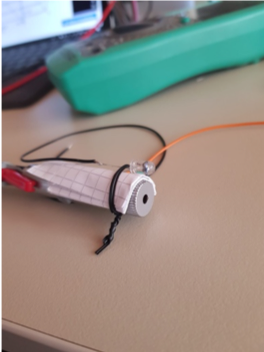
\includegraphics[width=0.25\textwidth]{images/Machbarkeitsstudie/Versuch1_Aufbau}	
	\caption{Versuchsaufbau}
	\label{versuch1_versuchsaufbau}
\end{figure}
\subsubsection{Messungen}
Insgesamt wurden vier Messungen durchgeführt.
\begin{enumerate}
	\item Photostrom im nicht abgedunkelten Raum
	\item Photostrom im abgedunkelten Raum
	\item Photostrom bei direktem Beleuchten mit einer Taschenlampe
	\item Photostrom bei direktem Beleuchten mit einem Laserpointer
	\item Photostrom bei Reflexion von einem Laserpointer
\end{enumerate}
Diese ersten vier Messungen sollen einen ersten Überblick über die Stärke des Photostroms geben und die Störeinflüsse des Umgebungslicht näher betrachten. Zudem kann über die fünfte Messung und die Variation des Abstandes der Reflexionsfläche Information darüber erlangt werden, wie groß die relative Änderungen des Photostroms bei relativer Änderung des Abstandes ist.
\subsection{Beobachtung}
Die größte Beobachtung, welche bei den Messungen gesehen werden konnte ist, dass der Photostrom nur im Bereich von wenigen $\mu A$ liegt.
\begin{enumerate}
	\item Nicht abgedunkelter Raum: $15\mu A$ 
	\item Abgedunkelter Raum: $3-5\mu A$  (sogenannter Dunkelstrom)
	\item Lichteinstrahlung Taschenlampe: $80\mu A$ 
	\item Lichteinstrahlung Laserpointer: $200\mu A$
\end{enumerate}
Diese ersten vier Messungen zeigten bereits, dass die Auftretenden Photoströme nur sehr gering sind und daher zusätzlich zu einer sehr schnellen Auswerteelektronik (Messung nach dem \ac{ToF} Prinzip) zudem eine sehr genaue Verstärkerschaltung nötig ist um gute Messergebnisse zu erzielen.
\begin{enumerate}
	\setcounter{enumi}{4}
	\item Bei Änderung des Abstandes der Reflexionsfläche in Messung fünf kann festgestellt werden, dass ein Abstand bis ca. $7cm$ detektiert werden kann. Die relative Änderung des Photostroms beträgt dabei $\frac{0,2}{7}\frac{\mu A}{cm}$
\end{enumerate}
\subsection{Erkenntnis}
Die größte Erkenntnis aus den Messungen des ersten Versuchs ist, dass Störende Lichteinflüsse so gut wie möglich eliminiert werden müssen. Dies kann z.B. durch Filter, welche nur das vom Laser ausgesandte Licht durchlassen, realisiert werden.\\
Ein Weiterer Punkt welcher festgestellt wurde ist, wie bereits schon erwähnt wurde, dass eine sehr Präzise Schaltung zu Feststellung der Photoströme nötig ist, da die Änderungen in sehr geringen Bereichen geschehen. Eine Lösung für dieses Problem könnte eine Verstärkerschaltung aus hochpräzisen Operationsverstärkern sein.\\
Der Dritte Punkt welcher in folgenden Messungen betrachtet werden sollte ist, dass eine Diode mit einer höheren Empfindlichkeit gegenüber der Lichteinstrahlung hat. Da wie beobachtet wurde die Reflektierte Lichtmenge sehr gering ist. Hier könnte beispielsweiße eine Avalanche Photodiode verwendet werden.

\section{Versuch 2: Weiterer Test handelsüblicher Photodioden}
\subsection{Versuchsaufbau}
\subsubsection{Verwendete Bauteile}
\begin{table}[H]
	\centering
	\caption{Bauteilliste Versuch 2}
	\begin{tabular}{|l|l|}
		\hline
		\textbf{Bezeichnung} & \textbf{Bauteil (Beschreibung)}
		\\\hline
		Photodiode & BPW34
		\\\hline
		Laserpointer & 1mW, 630-680 nm
		\\\hline
		Karton & 
		\\\hline
		Lupe &
		\\\hline
	\end{tabular}
\end{table}

\subsubsection{Verwendete Messgeräte}
\begin{table}[H]
	\centering
	\caption{Messgeräteliste Versuch 2}
	\begin{tabular}{|l|l|}
		\hline
		\textbf{Art des Messgeräts} & \textbf{Bezeichnung}
		\\\hline
		Digitalmultimeter & Agilent
		\\\hline
		DC Spannungsquelle & 
		\\\hline
	\end{tabular}
\end{table}
\subsubsection{Aufbau}
In die Seite des Kartons wurde je ein Loch für Laserpointer und Photodiode geschnitten und diese jeweils darin Angebracht. Im Karton wurde eine Reflexionsfläche im Abstand von $7cm$ aufgestellt und der Karton wurde verschlossen. Die Diode wurde mit einer Sperrspannung von $5V$ betrieben und das Digitalmultimeter in Reihe zur Photodiode geschaltet um analog zu Versuch 1 den entstehenden Photostrom zu messen. 
\subsubsection{Messungen}
\begin{enumerate}
	\item In der ersten Messung wurde die Photodiode zusammen mit dem Laserpointer im Dunklen getestet und der Photostrom im Dunkeln sowie bei Betätigung des Laserpointers gemessen.
	\item In einer zweiten Messung wurde vor der Photodiode eine Lupe Positioniert, sodass das Licht auf die Photodiode gebündelt wird. Es wird erwartet, dass durch die Lupe ein größerer Photostrom entsteht.
\end{enumerate}
\subsection{Beobachtung}
\begin{enumerate}
	\item Zunächst ist zu Beobachten, dass im Dunkeln ein Photostrom von $0,3\mu A$ durch die Photodiode fließt. Bei Betätigung des Laserpointers steigt der Photostrom um $0,2\mu A$ an. Wenn der Abstand Reflexionsfläche zu Laserpointer und Diode vergrößert wird, sinkt der Stromanstieg bei Betätigung des Laserpointers noch weiter ab. Diese Beobachtungen sind Analog zu den Beobachtungen aus Versuch 1.
	\item Bei Platzierung der Lupe vor der Photodiode ist ein stärkerer Stromanstieg bei Betätigung des Laserpointers zu Beobachten. Allerdings kann ist dieser Aufbau sehr schwer einstellbar. Hauptgrund dafür ist, dass der Laserpointer nun nichtmehr orthogonal zur Kartonwand aufgestellt werden kann, sondern in einem Winkel positioniert werden muss, damit die Reflexion möglichst exakt im Brennpunkt der Lupe positioniert ist. Dann kann auch der größtmögliche Stromanstieg beobachtet werden. 
\end{enumerate}
\subsection{Erkenntnis}
Die Erkenntnis aus dem zweiten Versuch ist, dass eine Optik vor der Photodiode eine größere Empfindlichkeit ermöglicht. Allerdings ist diese Optik auch sehr schwer einzustellen, da sich Einfallswinkel des Lichts mit steigender Entfernung kontinuierlich ändern. Zudem wurde Beobachtet, dass ein Dunkler Raum lediglich den Gesamtstrom reduziert, der Anstieg des Stroms bei Betätigung des Laserpointers bleibt gleich.\\
Die Bisherigen versuche beruhen auf dem \ac{ToF} Prinzip, da wir ständig versuchen eine Flanke des Photostroms zu erkennen. Ein Problem welches dabei bisher noch nicht betrachtet wurde ist wie im Kapitel \ref{subsec:tof_herausvorderungen} beschrieben, dass bei geringer Distanz die Lichtlaufzeit im Bereich weniger $ns$ liegt und daher eine sehr schnelle Auswerteelektronik nötig ist. Daher wird für weitere Test eine wie in Kapitel \ref{subsec:apd} \ac{APD} benötigt um wenige reflektierte Photonen besser detektieren zu können.
\section{Weiteres Vorgehen}
Wie bereits beschrieben sind weitere Versuche nur mit einer \ac{APD} sinnvoll. Da diese allerdings meist in Preisspektren > 100€ liegen wurden die Versuche eingestellt.
\subsection{Recherche}
Da es in unserem Unternehmen einige Abteilungen aus verschiedensten Bereichen gibt, welche sich mit Laserenfernungsmessung beschäftigen war der nächste Schritt Kontakt mit diesen Abteilungen aufzunehmen und die Pläne einen Eigenen \ac{LIDAR} Sensor zu entwickeln zu diskutieren. \\ 
Die Erkenntnis welche aus diesen Gesprächen gewonnen werden konnte ist, dass ohne \ac{APD} keines der drei in Kapitel \ref{sec:grund_lidar} vorgestellten Messverfahren realisierbar ist. Zudem wurden Hinweiße und Kritikpunkte an dem geplanten vorgehen geäußert und wichtige Hinweiße zur generellen Realisierung des Gesamtsystems angebracht. So zum Beispiel, dass bei einem \ac{LIDAR} Sensor nicht nur wichtig ist, was die minimale und maximale Messdistanz ist, sondern auch mit welcher Frequenz der Sensor diese Messergebnisse reproduzieren kann. Dies hat großen Einfluss auf Messgenauigkeit und Messdauer und ist daher ein weiterer Punkt welcher bei der Auswahl eines geeigneten Sensors betrachtet werden muss.
%Marcel
    %!TEX root = ../dokumentation.tex


\chapter{Matlab Modell}

Zur Konzeptionierung des Systems und zur Auswahl der benötigten Komponenten müssen einige Vorüberlegungen angestellt werden. Die geforderte Auflösung und Genauigkeit des Lidar-Systems, sowie die Maximalzeit für das Erstellen der Punktewolke sind ausschlaggebende Parameter für die Komponentenauswahl.

Die gefordete Genauigkeit sowie der vordefinierte Standardraum zur späteren Vermessung definieren hauptsächlich die Anforderungen an den Lidar Sensor. Bei gegebener Maximalzeit für einen Scan, muss zusätzlich die Messfrequenz des Sensors dementsprechend hoch sein. \\
Die Auflösung bestimmt die minimale erreichbare Schrittweite der Schrittmotoren. Dabei muss die nicht gleichmäßige Messpunkteverteilung an einer Wand berücksichtigt werden.

Das mittig im Raum aufgestellte Lidar-System nimmt eine Punktewolke des Raumes auf. Dazu soll sich der Sensor für jede Messung in zwei Achsen um einen vordefinierten Winkel weiterbewegen. Dies führt dazu, dass die Punkteverteilung trotz eines gleichbleibenden Winkels nicht homogen bleibt. 

Dies
Bsp nur Hotizontal:


Um die gefordete Auflösung auch noch an den am weitesten vom Lidar System entfernte Stellen zu erreichn, wird ein Matlab Modell erstellt. Bei diesem können Paramter….. eingestllet werden und man erhält die Punkteverteilung der Messung eximplarisch für eine Wand.

Matlab Modell einer Wand:

Schwierigkeiten:
Kompromiss finden, Punkte Zentral davor und 
Eindeutigkeit eines Punkes, bzw zuordnung zu einer Wand, Decke%Alexander
    %!TEX root = ../dokumentation.tex
\chapter{Mechanik}\label{chap:mechanik}

\section{Anforderungen}
Damit ein \acs{3D} Abbild eines Raumes erstellt werden kann, ist es erforderlich, dass ein \ac{LIDAR} Sensor möglichst leicht in mindestens zwei Achsen beweget werden kann. Deshalb muss im Rahmen dieses Projekts eine geeignete Mechanik entworfen werden, welche es ermöglicht, den Sensor auf zwei getrennt voneinander steuerbaren Achsen beliebig positionieren zu können. Damit eine solche Mechanik entworfen werden kann, müssen zuerst einige Rahmenbedingungen geklärt werden. Beispielsweise sollten die Motoren welche die Mechanik später antreiben vorher spezifiziert sein und die maximale Größe des Sensors bekannt sein. Natürlich sollte die Mechanik auch so entworfen werden, dass diese dann auch in der Praxis gefertigt werden kann.\\
Zur besseren Visualisierung und um genaue Zeichnungen anzufertigen, wurde ein \ac{CAD} Zeichenprogramm verwendet. 
\section{Entwurf}
Der gesamte Aufbau lässt sich in drei große Teile unterteilen. Einen oberen Aufbau, welcher das Kippen des Sensors übernimmt und einen Motor halten muss. Die Basis, welche sich um 360° Drehen lassen soll. Und den Rahmen, welcher die Steuerung und den zweiten Motor enthält. 

\subsection{Oberer Aufbau}
Für den oberen Aufbau der Mechanik gibt es mehrere Vorraussetzungen. Zuerst soll die gesamte Mechanik so funktionieren, dass der Sensor möglichst genau im Ursprung der Dreh- und Kippachse liegt, um spätere komplizierte Umrechnungen der Punktewolke zu verhindern. Dazu soll der Aufbau möglichst leicht und klein sein, damit die beschleunigte Masse und die damit verbundenen Trägheitskräfte möglichst gering sind. Damit werden unnötige Belastungen auf die Motoren vermieden. Außerdem müssen alle Leitungen, welche in dieser Aufbaute benötigt werden 360° drehbar sein, weshalb ein sogenannter Schleifring verwendet werden sollte. 
\begin{figure}[H]
	\centering
	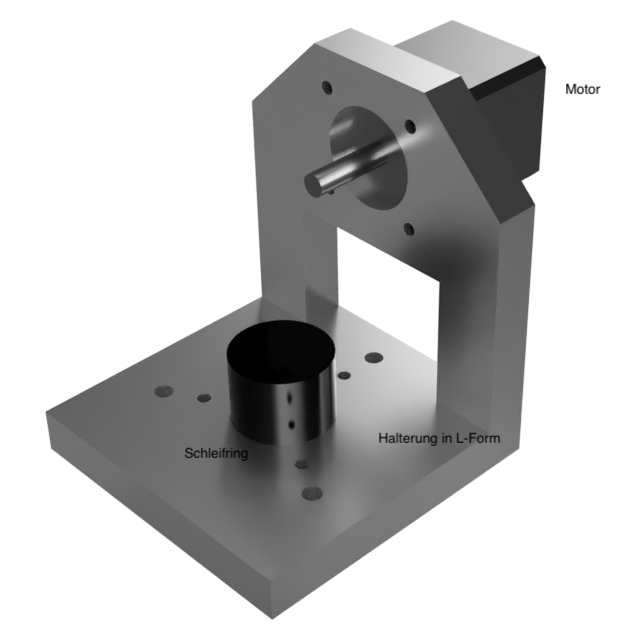
\includegraphics[width=0.75\textwidth]{images/Mechanik/ObererAufbau}
	\caption{Oberer Aufbau der Mechanik}
	\label{obereraufbau}
\end{figure}
Der Motor welcher in Abbildung \ref{obereraufbau} zu sehen ist, ist von der \ac{NEMA} genormt und hat den Namen \ac{NEMA} 11, die 11 verweist hierbei auf die Baugröße in diesem Fall $1,1"$ was ca. $28mm$ entspricht \cite{NEMA}. Außerdem ist in der Abbildung der Schleifring zu sehen, welcher später dazu dienen wird, dass alle Kabel des oberen Aufbaus um 360° drehbar sind. \\
Die Halterung in L-Form besteht aus zwei Teilen, welche aneinander geschraubt werden. Ein horizontales Teil, die Grundplatte, welche den Schleifring und die Verbindung zu den weiteren Teilen sicherstellt. Und ein vertikales Teil, welches den \ac{NEMA} 11 Motor in einer Vertiefung hält.\\
In Abbildung \ref{obereraufbau} fehlt allerdings ein weiteres Bauteil. Auf der Welle des Motors wird eine weitere Platte montiert, worauf später der \ac{LIDAR} Sensor montiert wird. Zur besseren Übersicht wurde in der gezeigten Ansicht auf diese Platte verzichtet.
\subsection{Basis}
Die Basis stellt die Verbindung zwischen dem oberen Aufbau und dem Rahmen dar. Die Basis ist die komplexeste Baugruppe der gesamten Mechanik, da sie den Antrieb und die Lagerung des oberen Aufbaus übernimmt. 
\begin{figure}[H]
	\centering
	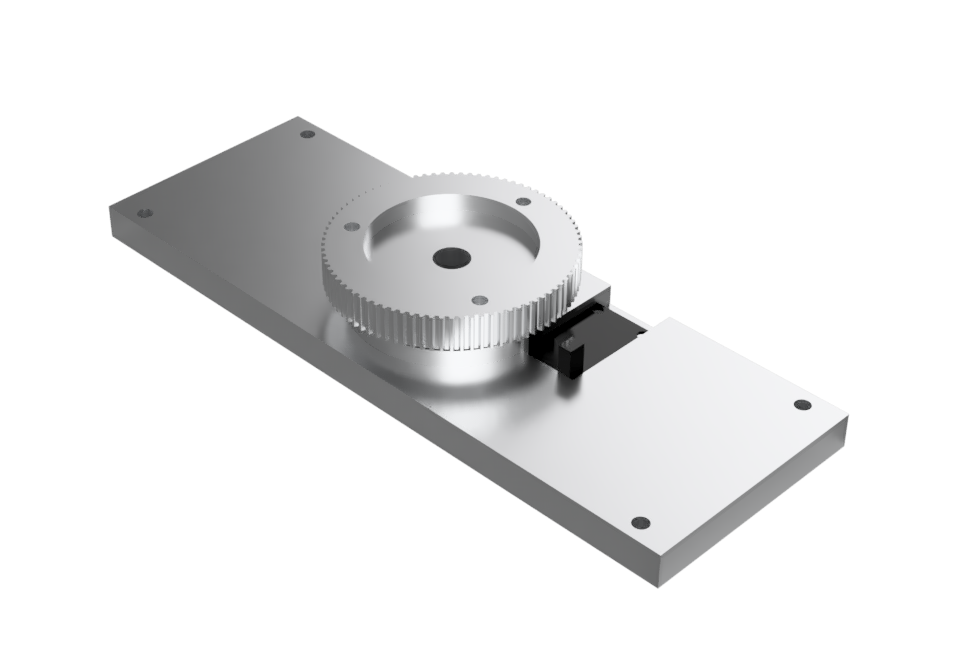
\includegraphics[width=0.75\textwidth]{images/Mechanik/Basis}
	\caption{Basis der Mechanik}
	\label{basis}
\end{figure}
Um die Lagerung herzustellen wird ein großes Kugellager mit einem Innendurchmesser von $22mm$ in die Verbindungsplatte (Abbildung: \ref{basis}) eingepresst. Der große Innendurchmesser des Kugellagers ist erforderlich, damit die Kabel durch dieses hindurch geführt werden können. Der Antrieb des oberen Aufbaus wird durch eine Zahnriemenscheibe hergestellt. Diese ist nach DIN 7721-2 T2,5 \cite{Tabellenbuch} entworfen da in dieser Anwendung eine große Anzahl an Zähnen gefordert ist, um eine höhere Winkelauflösung zu erhalten. Diese Zahnriemenscheibe wird 3D gedruckt. Mit dem gewünschten Mindestdurchmesser der Platte ergibt sich ein Umfang des Zahnrades von $66,3mm$ und eine Zahnanzahl von 84 Zähnen \cite{Tabellenbuch}. Um die Zahnriemenscheibe mit dem Kugellager zu verbinden, wird eine Adapterplatte verwendet, welche innen in das Kugellager eingepresst wird und anschießend mit Zahnriemenscheibe und mit dem oberem Aufbau verschraubt. Diese Adapterplatte hat ein durchgängiges Loch um die Kabel heraus zu führen. Zudem sitzt die Adapterplatte vertieft in der Zahnriemenscheibe, um die Baugröße kompakt zu halten und einen Formschluss zu erzeugen. Das letzte Bauteil der Basis ist die Lichtschranke welche zur Positionierung dient. Diese Lichtschranke sitzt vertieft in der Basisplatte, damit der sich drehende Teil darüber passt. Durch einen Zapfen an der 3D gedruckten Zahnriemenscheibe wird die Lichtschranke ausgelöst. 
\subsection{Rahmen}
Die dritte Baugruppe der Mechanik ist der Rahmen (Abbildung \ref{rahmen}). Dieser dient hauptsächlich dazu, eine stabile Befestigungsmöglichkeit für die Basis und den oberen Aufbau zu gewähren und die gesamte Elektronik zu ordnen. Zudem dient der Rahmen als Befestigungspunkt für den zweiten Motor. Der zweite Schrittmotor ist nach \ac{NEMA} 17 genormt mit einem Außenmaß von ca $41mm$. Dieser wird über einen Zahnriementrieb den gesamten oberen Aufbau  drehen. 
\begin{figure}[H]
	\centering
	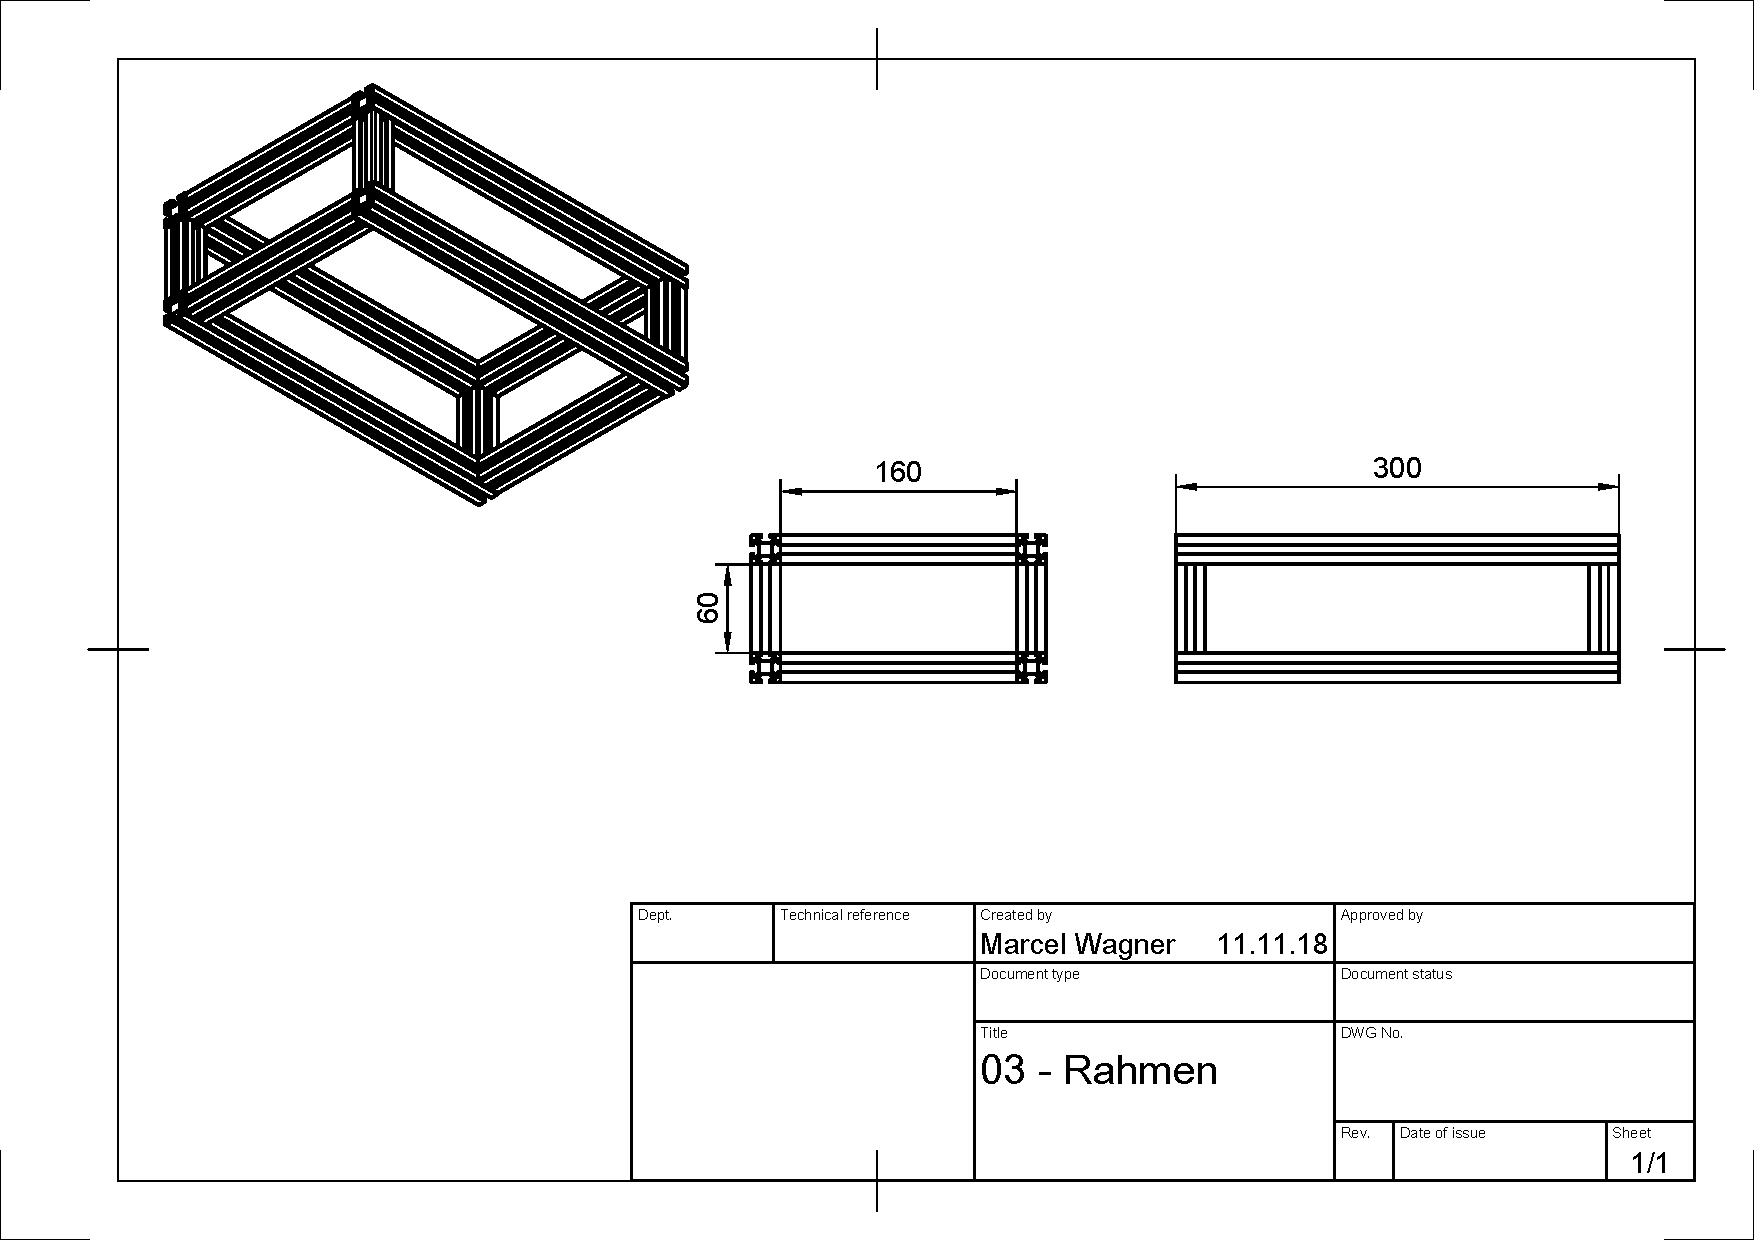
\includegraphics[width=0.75\textwidth]{images/Mechanik/Rahmen}
	\caption{Rahmen}
	\label{rahmen}
\end{figure}
Um das obere Ende der Welle des zweiten Schrittmotors auf die selbe Höhe wie die Oberkante der Zahnriemenscheibe zu bringen, ist eine weitere Halterung erforderlich. Auf der Motorwelle des \ac{NEMA} 17 Motors sitzt eine weitere Zahnriemenscheibe, allerdings in einem deutlich kleineren Durchmesser ($10,6mm$ Außendurchmesser, 14 Zähne). Durch die beiden verwendeten Zahnriemenscheiben ergibt sich ein Übersetzungsverhältnis welches im folgenden Berechnet wird:
\begin{equation}\formelentry{Berechnung Übersetzungsverhältnis \cite{Tabellenbuch}}
	i = \frac{z_a}{z_e} = \frac{84}{14} = 6
\end{equation} 
\begin{flalign*}
&i = \text{Gesamtübersetzungsverhältnis}&\\
&z_a = \text{Zähnezahl getriebene Scheibe}&\\
&z_e = \text{Zähnezahl treibende Scheibe}&
\end{flalign*}
Durch das erhöhte Übersetzungsverhältnis wird eine Verlangsamung der Drehbewegung erreicht. Dies ermöglicht eine noch exaktere Auflösung. Um eine komplette Drehung des Systems zu erreichen, muss sich der \ac{NEMA} 17 Motor sechs mal drehen, daher werden auch sechs mal so viele Schritte pro Drehung benötigt.\\
Außerdem wird für den gesamten Rahmen ein Aluminiumprofil mit Nutensteinen verwendet. Dies ermöglicht das Spannen des Riemens, welcher das System dreht. Zudem kann durch die Nuten im Aluminiumprofil einfach eine Bodenplatte zur Montage von Platine und Raspberry Pi eingesetzt werden. \\

\section{Umsetzung}
Nachdem die Zeichnungen von allen Bauteilen angefertigt und überprüft wurden, kann mit der Herstellung der einzelnen Bauteile begonnen werden. Fast alle selbst konstruierten Bauteile werden in Handarbeit aus Aluminium gefertigt. Dabei wurde durch Fräsen, Drehen und Bohren die gewünschte Form erreicht. Da wie bereits erwähnt die Basisplatte das komplexeste Bauteil ist, wird diese extra von einer \ac{CNC} Fräse gefertigt. Die Adapterplatte wird ebenfalls  \ac{CNC} gedreht, damit die Passform des Kugellagers erreicht wird und die Bauteile perfekt eingepresst werden können. Die Zahnriemenscheibe, welche auf der Basis montiert wird, wird \ac{3D} gedruckt, da ein herkömmliches Fertigungsverfahren mit den vorhandenen Mitteln nicht möglich ist.\\
\begin{figure}[H]
	\centering
	\includegraphics[width=0.75\textwidth]{images/Mechanik/Montiert}
	\caption{Mechanik mit montierter Elektronik}
	\label{montiert}
\end{figure}
Nach Fertigstellung aller Einzelteile kann die Mechanik zusammengebaut und die Elektronik eingebracht werden (Abbildung \ref{montiert}). Dabei werden noch einige kleinere Teile gefertigt, von welchen kein extra \ac{CAD} Modell erstellt wurde. So wird eine Halterung für den \ac{LIDAR} Sensor TF-Mini (Kapitel \ref{tf_mini}) aus einem Blech gebogen und gebohrt. Zusätzlich wird eine Platte zugeschnitten und gebohrt, welche in den unteren Teil des Rahmens eingesetzt werden kann, damit darauf die Platine und der Raspberry Pi montiert werden können. Nachdem auch diese kleineren Teile gefertigt sind, konnte die Mechanik final zusammengebaut werden. Dabei werden die Motoren an ihren vorgesehenen Plätzen montiert und die einzelnen Komponenten zusammengesetzt.
%Marcel
    %!TEX root = ../dokumentation.tex

\chapter{Elektronische Hardwarekomponenten}\label{chap:hardware}

Im folgenden Kapitel werden die elektronischen Hardwarekomponenten, sowie deren Verbindungen untereinander vorgestellt. 

Die einzelnen Komponenten lassen sich in drei große Funktionsbereiche klassifizieren:\\
Der erste Bereich beinhaltet die Distanzbestimmung. Diese wird durch den \ac{LIDAR} Sensor realisiert.\\
Der zweite Funktionsbereich beschäftigt sich mit dem Ausrichten des Sensors in zwei Achsen. Die Komponenten sind zwei Schrittmotoren und die damit verbundene Ansteuerung durch Motortreiber. \\
Die automatisierte Kalibrierung stellt den dritten Funktionsbereich dar. Dabei wird über eine Lichtschranke die horizontale Ausrichtung des Sensors bei jedem Start der Anwendung auf eine vordefinierte Ausgangsposition gesetzt. Dasselbe wird durch einen Gyrosensor für die vertikale Ausrichtung ermöglicht.

Als Rechen- und Steuereinheit für das gesamte System wird ein Raspberry Pi verwendet. Dieser bietet sich aufgrund des geringen Preises, der vielen \ac{GPIO} Pins und der Unterstützung aller benötigten Datenübertragungsprotokolle an. Zudem reicht die Rechenleistung für das Ansteuern aller Komponenten, sowie für das Auswerten und Speichern der Messdaten aus.\\

\section{Funktionseinheit Distanzbestimmung}

Bei der Auswahl des \ac{LIDAR} Sensors spielen Preis, Verfügbarkeit, Messfrequenz, Auflösung, Genauigkeit und messbare Entfernung eine Rolle. Im Folgenden werden zwei ausgewählte Sensoren vorgestellt. 


\subsection{TF Mini \ac{LIDAR}}\label{tf_mini}


\begin{wrapfigure}{r}{5cm}
	\vspace{-22pt}
	\hspace{5mm}
	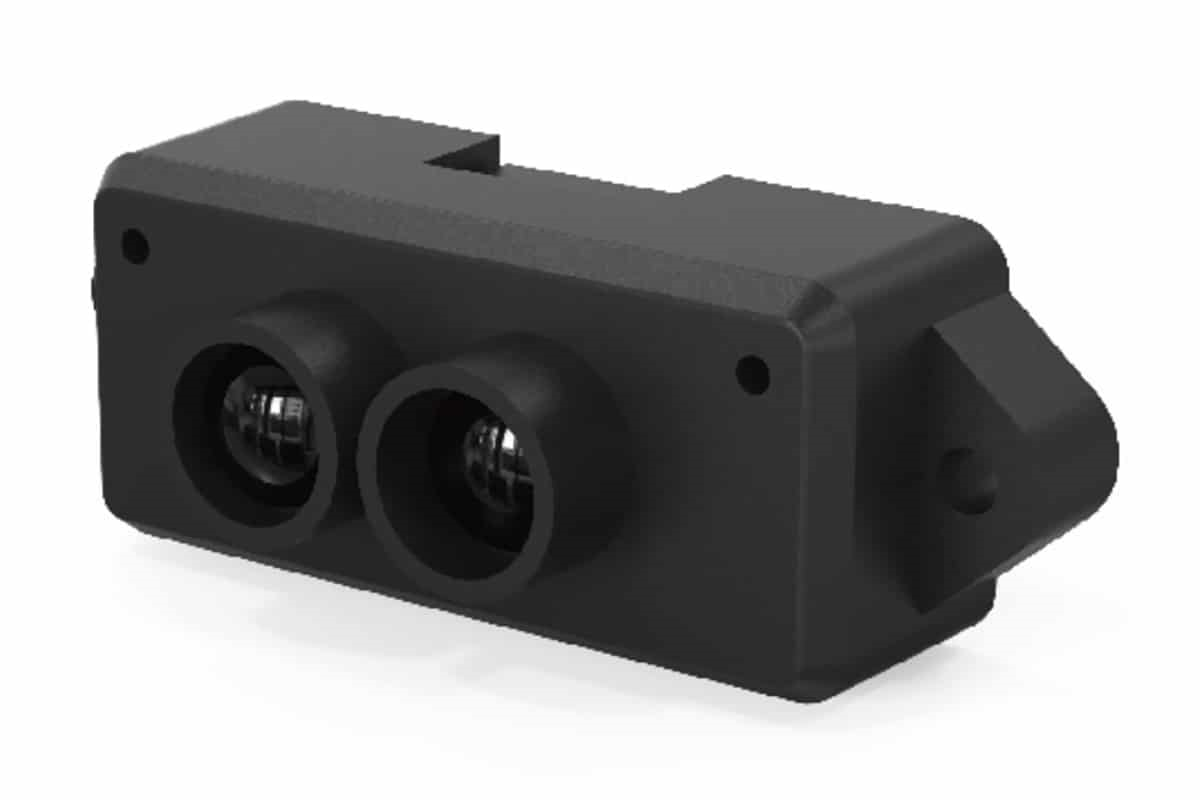
\includegraphics[width=4cm]{images/Hardware/TFmini.png}
	\caption{TF Mini}
	\vspace{-10pt}
	
\end{wrapfigure}

Als Hauptsensor wird ein „TF Mini \ac{LIDAR}“ von dem Hersteller „Seeedstudio“ verwendet. Dieser misst Entfernungen mit dem Prinzip der Phasendifferenz wie in Kapitel \ref{sec:phasenverschiebung} beschrieben.\\
Der Arbeitsbereich ist zwischen 30 cm und 1200 cm mit einer Auflösung von 1 cm. Bei Entfernungen kleiner als 600 cm beträgt die Messungenauigkeit 1\%. Zwischen 600 cm und 1200 cm 2\%. Die Messfrequenz beträgt maximale 100 Hz.\\
Der Sensor arbeitet mit einer Versorgungsspannung von 4,5 V – 6 V bei einem durchschnittlichen Stromverbrauch von 120 mA. Das Kommunikation läuft über eine \ac{UART} Schnittstelle mit einer Logikspannung von 3,3 V. \cite{TFMINI}

Dieser Sensor wurde ausgewählt, da das Preis-Leistung Verhältnis und die Verfügbarkeit sehr gut ist. Zudem reicht der messbare Bereich für den zuvor definierten Standardraum aus. Die Kommunikation über \ac{UART} ist mit dem Raspberry Pi realisierbar. Sensoren mit einer deutlich höheren Messfrequenz sind um ein vielfaches teurer, weshalb aufgrund der Anforderung eines kostengünstigen Systems die Messfrequenz von 100 Hz  ausreichend sein muss. Zusätzlich wird dadurch nicht die Qualität des Ergebnisses beeinflusst. Die niedrigere Messfrequenz beeinträchtigt nur die Geschwindigkeit, mit der ein Raum vermessen werden kann. \\
Der Sensor ist 42 x 15 x 16 mm groß, wodurch er sehr gut auf der dafür vorgesehenen Aluminiumhalterung montiert werden kann. 


\subsection{VL53L1X} \label{sec:VL53L1X}

Als alternativer, kostengünstigerer Sensor wird der \ac{ToF} Sensor VL53L1X verwendet. Der Sensor nutzt das Prinzip der Lichtlaufzeitmessung. Es können Distanzen von bis zu 400 cm mit einer maximalen Frequenz von 50 Hz gemessen werden. Die Kommunikation erfolgt über \ac{I$^{2}$C}. \\
Die Versorgungsspannung liegt zwischen 2,6 und 3,5 V. Sowohl der Erfassungswinkel als auch der interessante Entfernungsbereich kann softwaretechnisch eingestellt werden. \cite{VL53L1X}

Der Arbeitsbereich ist von dem eingestellten Distanzmodus abhängig. Man kann wie in Tabelle \ref{distanzmodi} dargestellt zwischen drei Modi auswählen. Die Tabelle zeigt zudem die maximal messbare Distanz für den jeweiligen Modus in Abhängigkeit von dem Umgebungslicht. Der Modus für kurze Distanzen ist  Umgebungslicht unempfindlich. Bei den Modi für mittlere bis hohe Distanzen reagiert der Sensor sehr stark auf Umgebungslicht. Die maximal zu messende Distanz beträgt bei hohem Umgebungslicht nur noch ca. 75 cm. 

\begin{table}[H]
	\centering
	\caption{Distanzmodi VL53L1X}
	\begin{tabular}{|c|c|c|}
		\hline
		\textbf{Distanz Modus} 
		& \begin{tabular}[x]{@{}c@{}}\textbf{max. Distanz}\\\textbf{(abgedunkelt)}\end{tabular}
			& \begin{tabular}[x]{@{}c@{}}\textbf{max. Distanz}\\\textbf{(Umgebungslicht)}\end{tabular} 	 \\ \hline
		Kurz	&  136 cm		& 135 cm\\ \hline
		Mittel  &  290 cm	  	& 76 cm	\\ \hline
		Lang 	&  360 cm		& 73 cm	\\ \hline
				
		\end {tabular}
	
	\label{distanzmodi}
\end{table}

In der späteren Anwendung wird der Modus für große Distanzen benötigt. Daher sollten während der Messung potentielle Fehlerquellen durch Umgebungslicht vermieden werden.

Die Genauigkeit der Messung hängt wie in Abbildung \ref{VL53L1X} zu sehen von der Messfrequenz ab. Die Abbildung zeigt das Verhalten bei unterschiedlichen Frequenzen. Dabei wird auf die Genauigkeit des Sensors, die maximal messbare Entfernung und die Replizierbarkeit der Messwerte eingegangen. ''Timing Budget'' ist dabei die Zeit, die benötigt wird, um einen Messwert aufzunehmen. Die Frequenz lässt sich daraus mit dem Kehrbruch berechnen.
''STDEV'' steht für ''standard deviation'' oder auch Standardabweichung. Dieser Wert gibt die Streubreite der gemessenen Werten um den tatsächlichen Wert an. Je höher dieser Wert, desto geringer ist die Genauigkeit des Sensors. \\ 
 

\begin{figure}[H]
	\centering
	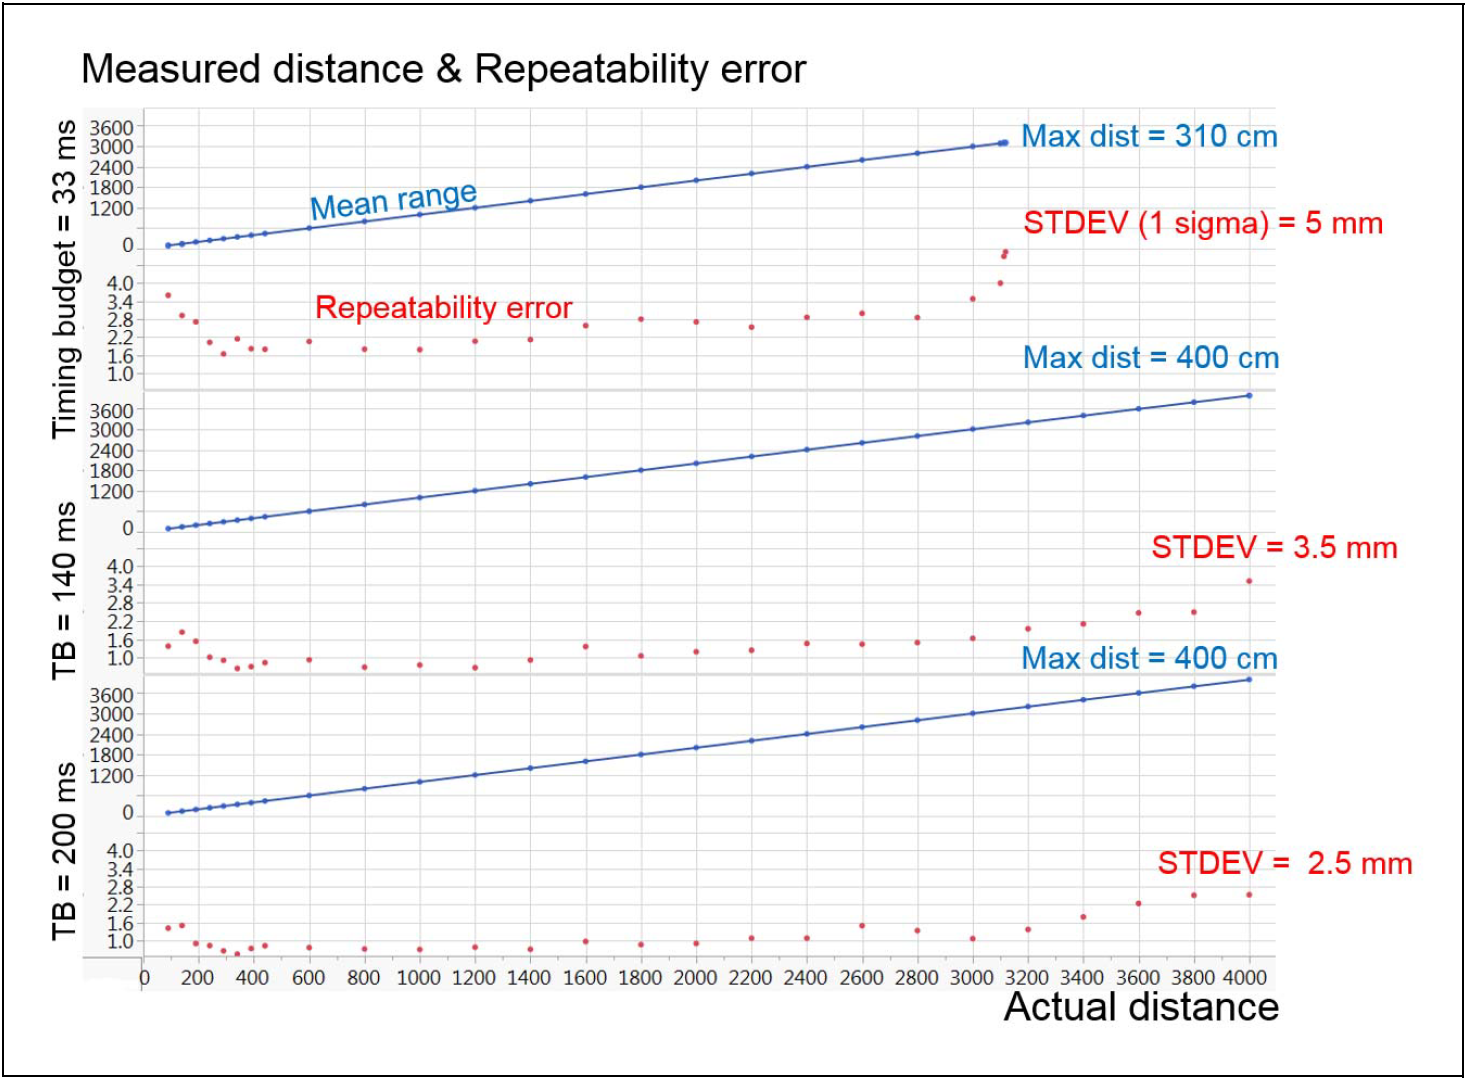
\includegraphics[width=0.75\textwidth]{images/Hardware/VL53L1X_Messfrequenz}
	\caption{Abhängigkeit der Genauigkeit des VL53L1X Sensors von der Messfrequenz}
	\label{VL53L1X}
\end{figure}

Das obere Diagramm in Abbildung \ref{VL53L1X} zeigt das Verhalten des Sensors bei einer Messfrequenz von 30,3 Hz. Bei dieser Frequenz kann unter perfekten äußeren Bedingungen nur eine maximale Distanz von 310 cm erreicht werden. Zudem ist die Genauigkeit des Sensors am schlechtesten. Mit kleiner werdender Messfrequenz nimmt die Genauigkeit zu und die maximal messbare Distanz beträgt bei entsprechenden Messverhältnissen 400 cm. Gute Messverhältnisse sind möglichst wenig Umgebungslicht und gut reflektierende Gegenstände. \cite{VL53L1X_manual}


Der Sensor ist mit 4,9 x 2.5 x 1.56 mm sehr klein. Zudem müssen 12 Pins auf der Unterseite verlötet werden. Aufgrund mangelnder Ausrüstung zum Löten solcher Chips wird ein bereits verbauter Sensor auf einer Platine verwendet. Auf der Platine sind zudem benötigte Widerstände und Kondensatoren verbaut. Werden die 12 herausgeführten Pins der Platine verwendet, ist der Sensor um 90 Grad vertikal verdreht und kann nicht auf der dafür vorgesehenen Adapterplatte der Mechanik montiert werden. Deshalb wird eine weiter Adapterplatine entworfen, auf welche die Platine mit dem Sensor aufgesteckt werden kann und somit um 90 Grad gedreht wird.


Im Vergleich zum ''TF Mini LIDAR'' Sensor muss beim ''VL53L1X'' auf äußere Einflüsse wie Umgebungslicht oder Reflexionsverhalten der Oberflächen geachtet werden. Zudem ist die maximal messbare Entfernung laut Spezifikation zu gering. Da jedoch ein möglichst kostengünstiges System entwickelt werden soll, wird der Sensor trotzdem für Tests verwendet, da es der kostengünstigste Sensor auf dem Markt ist, welcher den Anforderungen annähernd entspricht.



\subsection{Tabellarischer Vergleich der Sensoren}

Eine tabellarischer Auflistung der relevanten Daten der beiden ausgewählten Sensoren vereinfacht den direkten Vergleich für spätere Auswertungen. Neben vor allem technischen Daten wird auch der Preis in Tabelle \ref{vergleich} aufgenommen.

\begin{table}[H]
	\centering
	\caption{Tabellarischer Vergleich TF Mini und VL53L1X}
	\begin{tabular}{|c|c|c|}
		\hline
		\textbf{} 				& \textbf{Tf Mini LIDAR}	& \textbf{VL53L1X} 	 \\ \hline
		Preis [€]				&  35-40					& 10			\\ \hline
		Arbeitsbereich [cm]		&  30 - 1200   				& 3-400			\\ \hline
		max. Messfrequenz [Hz]	&  100						& 50 			\\ \hline
		Messungenauigkeit [\%]	&  1-2 						& <1			\\ \hline
		Schnittstelle 			&  \ac{UART}				& \ac{I$^{2}$C}\\ \hline
 		
	\end {tabular}
	\label{vergleich}
\end{table}


Es gilt zu beachten, dass sich beim Sensor VL53L1X einige Werte gegenseitig ausschließen. So ist bei einer Messfrequenz von 50 Hz beispielsweise keine Entfernung von 400 cm messbar. Diese gegenseitigen Einschränkungen sind in Kapitel \ref{sec:VL53L1X} aufgeführt und erklärt.

 

\section{Funktionseinheit Ausrichtung des Sensors}

Der Sensor wird durch je einen Schrittmotor in der Horizontalen als auch Vertikalen bewegt. Die vertikale Ausrichtung erfolgt dabei direkt. Der Sensor ist über eine Adapterplatte direkt mit der Welle des Schrittmotors verbunden. Dadurch werden Bewegungen des Schrittmotors 1:1 auf den Sensor übertragen.\\ 
Die horizontale Ausrichtung erfolgt zusätzlich über einen Zahnriementrieb zur Kraftübertragung. Das Übersetzungsverhältnis entspricht 6:1.  

\subsection{Schrittmotoren}
Das Drehen der Basis übernimmt ein bipolarer Hybrid-Schrittmotor der Bauform \ac{NEMA} 17 und einem Vollschrittwinkel von 1.8°. Der Maximalstrom beträgt 1.2 A pro Phase bei einer Spannung von 4V.\\ 
Dieser Motor wurde gewählt, da er genug Drehmoment aufbringt, um die gesamte Basis drehen zu können. Das hohe Haltemoment von 3,2 $\frac{kg}{cm}$ verhindert ungewolltes Verdrehen der Basis während der Messung. Dadurch ist das System fehlerresistenter auf äußere Einflüsse. \cite{NEMA17} 


Zum Kippen des \ac{LIDAR} Sensors wird ebenfalls ein bipolarer Hybrid-Schrittmotor verwendet. Dieser Motor befindet sich auf der sich drehenden Basis. Der Schwerpunkt des Motors befindet sich dabei unumgänglich einige Zentimeter neben der Drehachse. Deswegen sollte der Motor möglichst wenig Gewicht aufweisen, um die bei Drehung entstehende Unwucht so klein wie möglich zu halten.
Zum vertikalen Kippen des Sensor wird nicht so viel Kraft benötigt, als für das Drehen der gesamten Basis. Auf Grund dessen reicht die Bauform \ac{NEMA} 11. Diese Bauform ist deutlich kleiner und dadurch leichter.
Das Haltemoment reicht aus, um ungewolltes vertikales Verdrehen zu vermeiden.


\subsection{Schrittmotortreiber} \label{sec:Schrittmotortreiber}
Zur Ansteuerung der Schrittmotoren wird der Schrittmotortreiber A4988 verwendet. Dieser ist bereits auf einer Trägerplatine mit Teilen der äußeren Beschaltung verbaut.\\
Der Motortreiber ermöglicht es, bipolar Schrittmotoren mit eine Motorspannung von 8 V - 35 V mit einem maximalen Phasenstrom von 2 A anzusteuern. \cite{A4988}\\ 
Mit dem Motortreiber sind Mikroschritte realisierbar. Dabei sind halb, viertel, achtel und sechzehntel Schritte möglich. Der maximale Ausgangsstrom ist über einen Potentiometer auf der Trägerplatine stufenlos einstellbar. 

\begin{figure}[H] 
	\centering 
	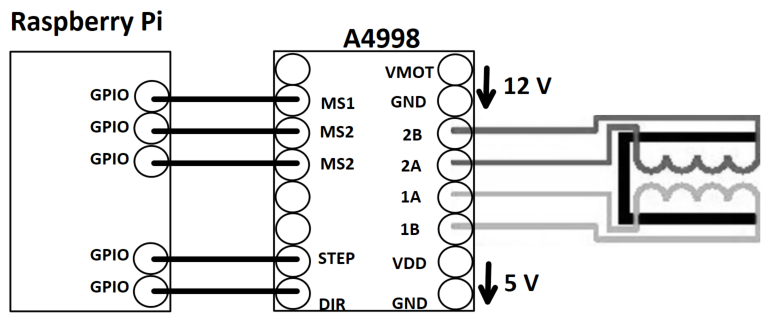
\includegraphics[width=0.7\textwidth]{images/Hardware/A4988} 
	\caption{Schematische Beschaltung der A4988 Trägerplatine} 
	\label{A4988} 
\end{figure} 



Der Motor wird spulenweise an den Motortreiber angeschlossen. Dabei wird Pin 1A und 1B sowie 2A und 2B über jeweils eine Spule des Schrittmotors verbunden.
Die Versorgungsspannung wird über ein 12 V Tischnetzteil bereitgestellt. Die Versorgungsspannung wird zusätzlich mit einem Stützkondensatoren geglättet. Der Kondensator hat eine Kapazität von 150 $\mu$F.
Als Kontrolleinheit für den Motortreiber dient ein Raspberry Pi. Die Logikspannungsversorgung des Treibers wird mit 5 V gespeist.\\ 
Die Anschlüsse ''STEP'', ''DIR'', sowie ''MS1-MS3'' werden mit \ac{GPIO}’s verbunden. Der Logikpegel an dem DIR-Pin legt die Bewegungsrichtung des Motors fest. Ein alternierendes Digitalsignal am STEP-Pin führt zur Rotation des Motors. Pro steigende Flanke dreht sich der Motor um die mit MS1-MS3 eingestellte Schrittweite weiter. \\  
MS1-MS3 dienen zum Einstellen der Schrittweite. Die Kombination der Logiklevel entscheidet dabei über die Schrittweite. Theoretisch wären somit $2^{3}$ Kombinationen möglich. Es werden jedoch nur fünf Einstellungen benötigt. Die verfügbaren Kombinationen sind in Tabelle \ref{Mikrostepping} aufgelistet. In der Tabelle ist der Zusammenhang von Schrittweite und Logiklevel an MS1-MS3 dargestellt. 


\begin{table}[H]
	\centering
	\caption{Schrittweite}
	\begin{tabular}{|c|c|c|c|}
		\hline
		\textbf{MS1} & \textbf{MS2}	& \textbf{MS3} 		& \textbf{Auflösung} \\ \hline
		Low & Low	& Low		& Vollschritt\\ \hline
		High & Low 	& Low  		& Halbschritt	\\ \hline
		Low & High  & Low 		& viertel Schritt 	\\ \hline
		High & High	& Low 		& achtel Schritt 	\\ \hline
		High & High	 &  High	& sechzehntel Schritt	\\\hline
	
	\end {tabular}
	\label{Mikrostepping}
\end{table}



Um Beschädigungen an den Schrittmotoren zu vermeiden, muss der maximale Strom durch die Spulen begrenzt werden. Diesen kann man über einen Potentiometer auf der Oberseite der Trägerplatine einstellen. Dafür wird die Referenzspannung zwischen dem Potentiometer und Masse gemessen. Mit der Formel: 

\begin{equation}\formelentry{Berechnung maximaler Strom für Schrittmotoren \cite{A4988}} 
I_{max} = U_{Ref} \cdot 2 
\end{equation}  
\begin{flalign*} 
&I_{max} = \text{maximaler Strom pro Phase [A]}&\\ 
&U_{Ref} = \text{Referenzspannung zwischen Potentiometer und Masse [V]}& 
\end{flalign*} 

wird der maximale Strom bei gegebener Spannung berechnet. Durch verändern des Widerstandes des Potentiometer verändert sich die Referenzspannung und der Wert des maximalen Stroms ändert sich. \\ 
Unterschiedliche Bauweisen der Bauteile führen oftmals dazu, dass die Formel nur als grober Richtwert gewertet werden kann. Nach der groben Einstellung des Stromlimits mithilfe der Formel sollte der Strom bei aktivem Motor gemessen und gegebenenfalls noch angepasst werden.\\ 
Das Verändern der Schrittweiten hat ebenfalls einen Einfluss auf den maximalen Strom. Deshalb sollte der Treiber auf die Schrittweite eingestellt werden, bei der der maximale Strom fließt.\\ 
Pro Motor wird ein Motortreiber verwendet. 



\section{Funktionseinheit Kalibrierung}

Sowohl die horizontale als auch vertikale Ausgangsposition soll beim Starten einer Messung vom System selbständig gefunden werden. Dabei wird der Sensor möglichst parallel zum Rahmen und dem Boden ausgerichtet. Dadurch wird spätere Nachbearbeitung der Daten hinsichtlich Ausrichtung überflüssig, was Zeit und Aufwand spart. Wird die Anfangskalibrierung der Achsen nicht oder nur ungenau vorgenommen, ist die spätere 3D Darstellung um einen bestimmten Winkel verdreht.

\subsection{Lichtschranke}
Zum automatischen Positionieren der Basis wird eine Infrarot Lichtschranke verwendet. Diese befindet sich unter der Zahnriemenscheibe und detektiert das Durchlaufen des daran befestigten Kalibrierzapfens. Lichtschranke und Zapfen sind so zueinander ausgerichtet, dass beim Detektieren des Zapfens der Sensor parallel zum Rahmen steht.\\ 
Auf dem Lichtschrankenmodul ist ein LM393 Komparator \ac{IC} verbaut. Das Modul benötigt eine Versorgungsspannung von 5 V. Der Ausgangspin wird mit einem \ac{GPIO}-Pin des Raspberry Pis verbunden. An diesem Ausgang liegt ein digitales Signal an, welches den Status der Lichtschranke darstellt. Liegt ein High-Signal an, befindet sich etwas zwischen der Lichtschranke und sie ist unterbrochen. Wechselt dieser Wert auf einen Low-Pegel, so ist sie nicht mehr unterbrochen \cite{LM393}. 
\subsection{Gyrosensor}
Die Kalibrierung in vertikaler Richtung soll über eine Gyroskop realisiert werden. Dieses muss die absolute Ausrichtung in der vertikalen Richtung detektieren können. \\ 
Als Sensor wird der Beschleunigungssensor MPU 6050 verwendet. Dieser benötigt eine Versorgungsspannung von 3,3 V. Die Messwerte werden über \ac{I$^{2}$C} ausgegeben.\cite{MPU-6050} Sowohl Spannungsversorgung als auch Takt- und Datenleitung werden direkt mit dem Raspberry Pi verbunden. \\ 
Der Sensor wird vor dem Befestigen an der Unterseite der Adapterplatte auf seine Funktion überprüft. Dabei wird festgestellt, dass der Sensor nicht die benötigte Genauigkeit liefert, um die genaue Positionierung des Sensors in vertikaler Richtung zu gewährleisten. \\
Die vertikale Ausrichtung erfolgt während der Tests manuell.


\section{Platinen}

Um einen Wechsel der Rechen- und Steuereinheit zu ermöglichen, wird eine Platine entworfen, die über ein 40 adriges Flachbandkabel direkt mit allen Pins des Raspberry Pi's verbunden werden kann. Auf der Platine sind zudem Motortreiber und Spannungsversorgung verbaut. Alle benötigten Schnittstellen und zusätzliche \ac{GPIO}’s sind durch die Platine mit Stiftleisten verbunden.\\
Für die Schaltplan- und Layouterstellung wird die Software ''EAGLE'' von Autodesk verwendet.


\subsection{Abwärtswandler} 

Einige Komponenten benötigen eine Spannung von 5V. Die Versorgungsspannung von 12 V muss somit verringert werden. Dazu wird ein Abwärtswandler des Typs MH-Mini-360 verwendet. Über ein Potentiometer auf der Oberseite des Moduls kann die Ausgangsspannung stufenlos eingestellt werden.

\subsection{Schaltplan} \label{sec:Schaltplan} 
Abbildung \ref{spannung} zeigt die Beschaltung der Spannungsversorgung und Spannungswandlung. Über den Hohlstecker (links) wird die Platine mit 12 V versorgt. Der 150 $\mu$F Kondensator dient zur Glättung der Eingangsspannung. Der Abwärtswandler wird mit den 12 V Eingangsspannung verbunden. Der Ausgang wird auf 5 V eingestellt. \\
Sowohl die 12 V als auch die 5 V können über Kurzschlussbrücken bzw. Schalter von der nachfolgenden Schaltung getrennt oder verbunden werden.    

\begin{figure}[H]
	\centering
	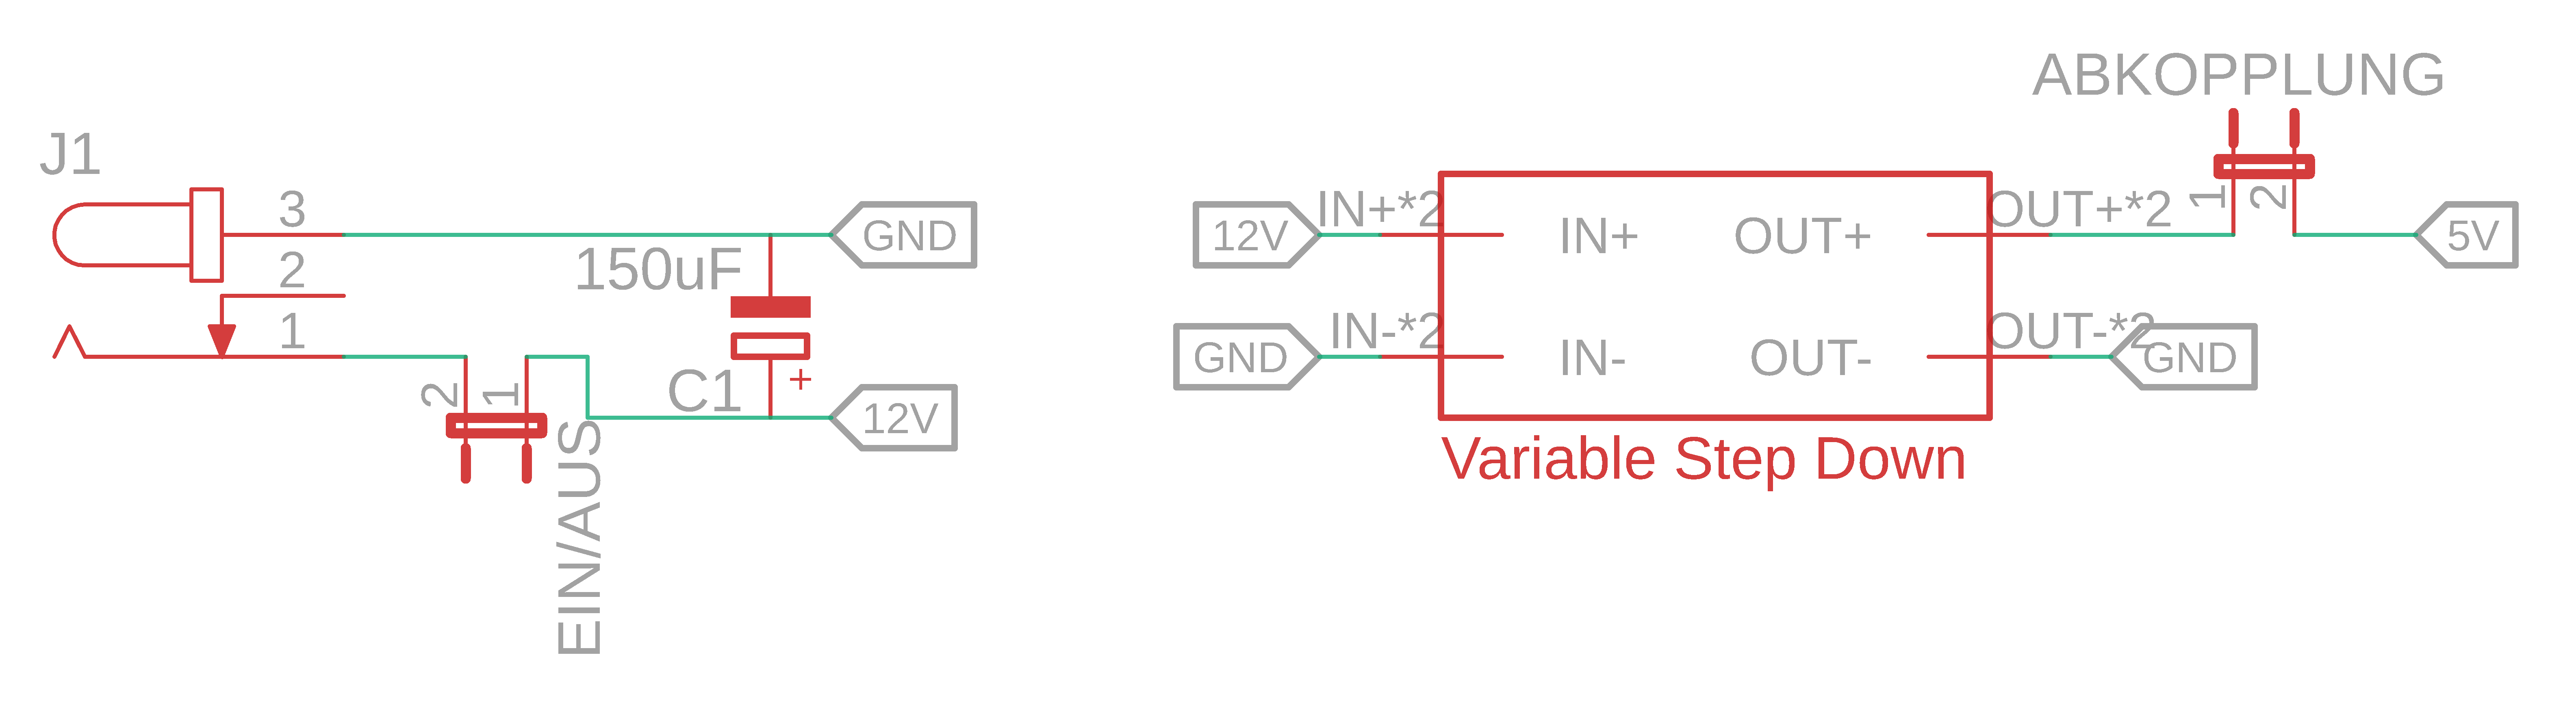
\includegraphics[width=0.6\textwidth]{images/Hardware/Schaltplan/Spannung}
	\caption{Schaltplan: Spannungsversorgung}
	\label{spannung}
\end{figure}

Abbildung \ref{driver} zeigt die Beschaltung der Motortreiber wie in Kapitel \ref{sec:Schrittmotortreiber} beschrieben. Die vier Anschlüsse für die Motorspulen werden mit Stiftleisten realisiert, an denen man den Motor später anstecken kann.

\begin{figure}[H]
	\centering
	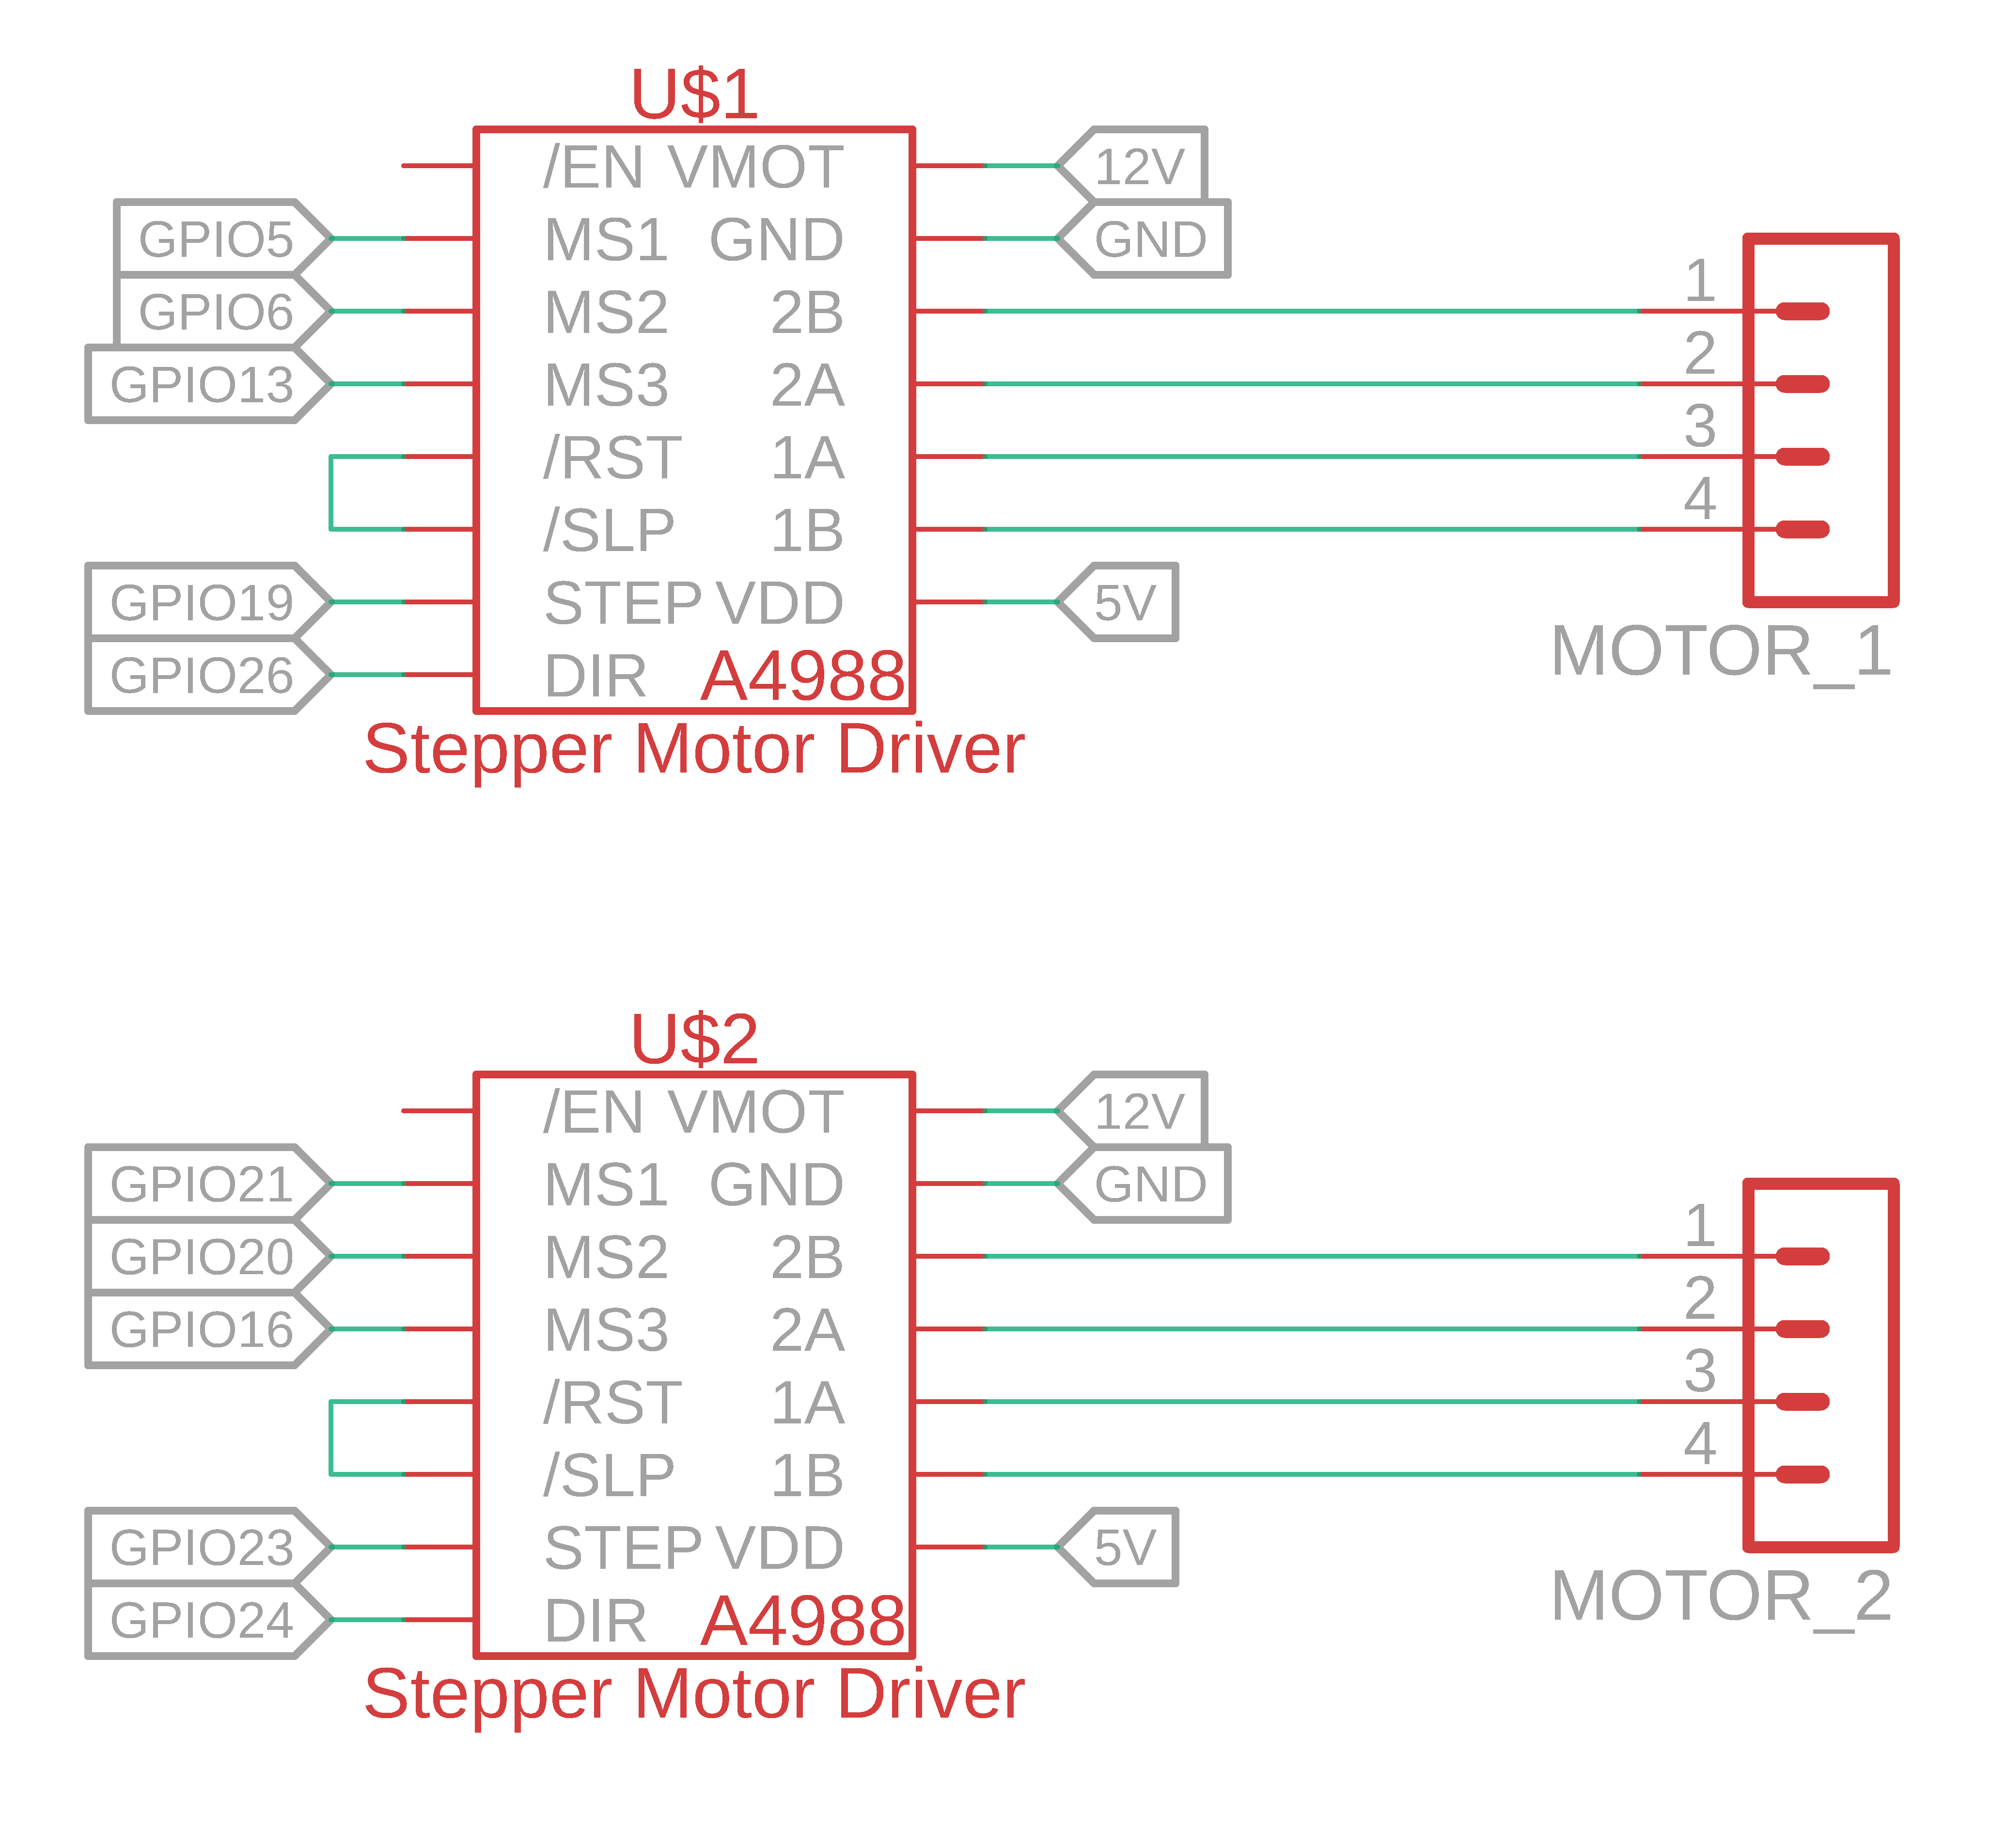
\includegraphics[width=0.6\textwidth]{images/Hardware/Schaltplan/Driver}
	\caption{Schaltplan: Motortreiber}
	\label{driver}
\end{figure}

Abbildung \ref{schnittstellen} zeigt die Verbindung zum Raspberry Pi und die verschiedenen Schnittstellen. An den 40 Pins (links) kann ein Raspberry Pi über ein Flachbandkabel verbunden werden. \\
Die benötigten Schnittstellen werden über Stiftleisten zugänglich gemacht. Es werden eine \ac{UART}-, eine \ac{SPI}- und drei \ac{I$^{2}$C}- Schnittstelle verbunden. Es werden mehr Schnittstellen zugänglich gemacht, als benötigt. Dies garantiert Flexibilität für Weiterentwicklungen. \\
Ein weiterer Anschluss ist mit den verschiedenen Spannungen der Platine verbunden. 

\begin{figure}[H]
	\centering
	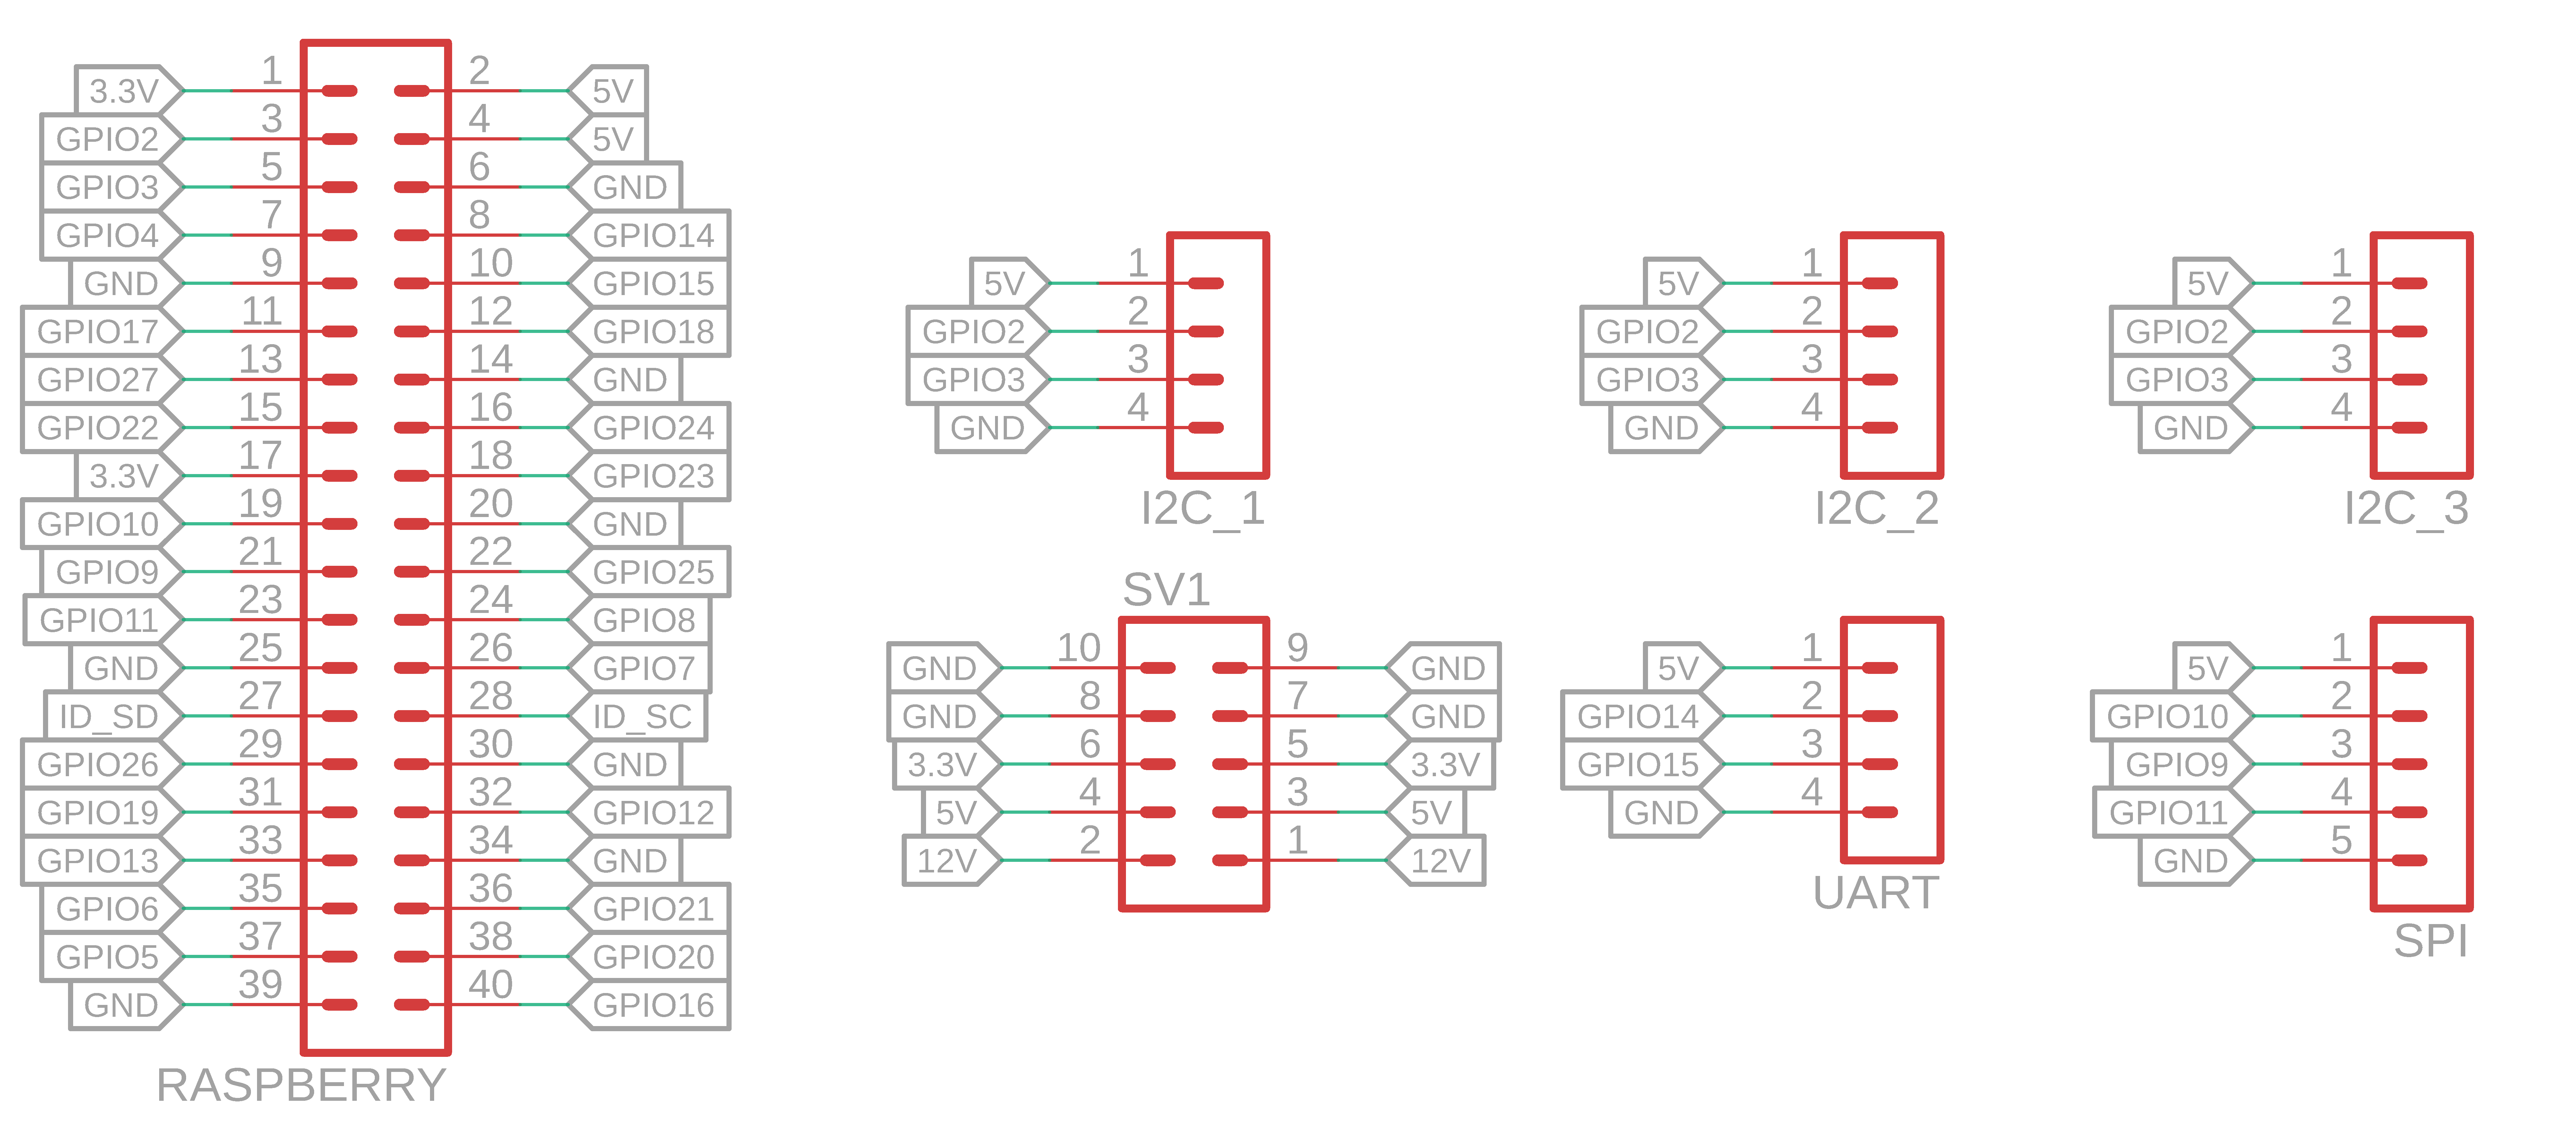
\includegraphics[width=0.6\textwidth]{images/Hardware/Schaltplan/Schnittstellen}
	\caption{Schaltplan: Schnittstellen}
	\label{schnittstellen}
\end{figure}

Abbildung \ref{leds} zeigt die Schaltungen für den optionalen Anschluss von Status \acp{LED} und einem Luftkühler über Pins. Eine Status-\ac{LED} kann über einen strombegrenzenden Widerstand mit 5 V verbunden werden. Steht das System unter Spannung, leuchtet die \ac{LED}. Eine weitere \ac{LED} kann mit dem Raspberry Pi über einen Transistor angesteuert werden. Die Funktion der \ac{LED} kann im Code direkt definiert werden.\\
An zwei weiteren Pins kann ein Luftkühler an 12 V angeschlossen werden. Die Steuerung des Kühlers ist über einen Transistor mit dem Raspberry Pi möglich.
  
\begin{figure}[H]
	\centering
	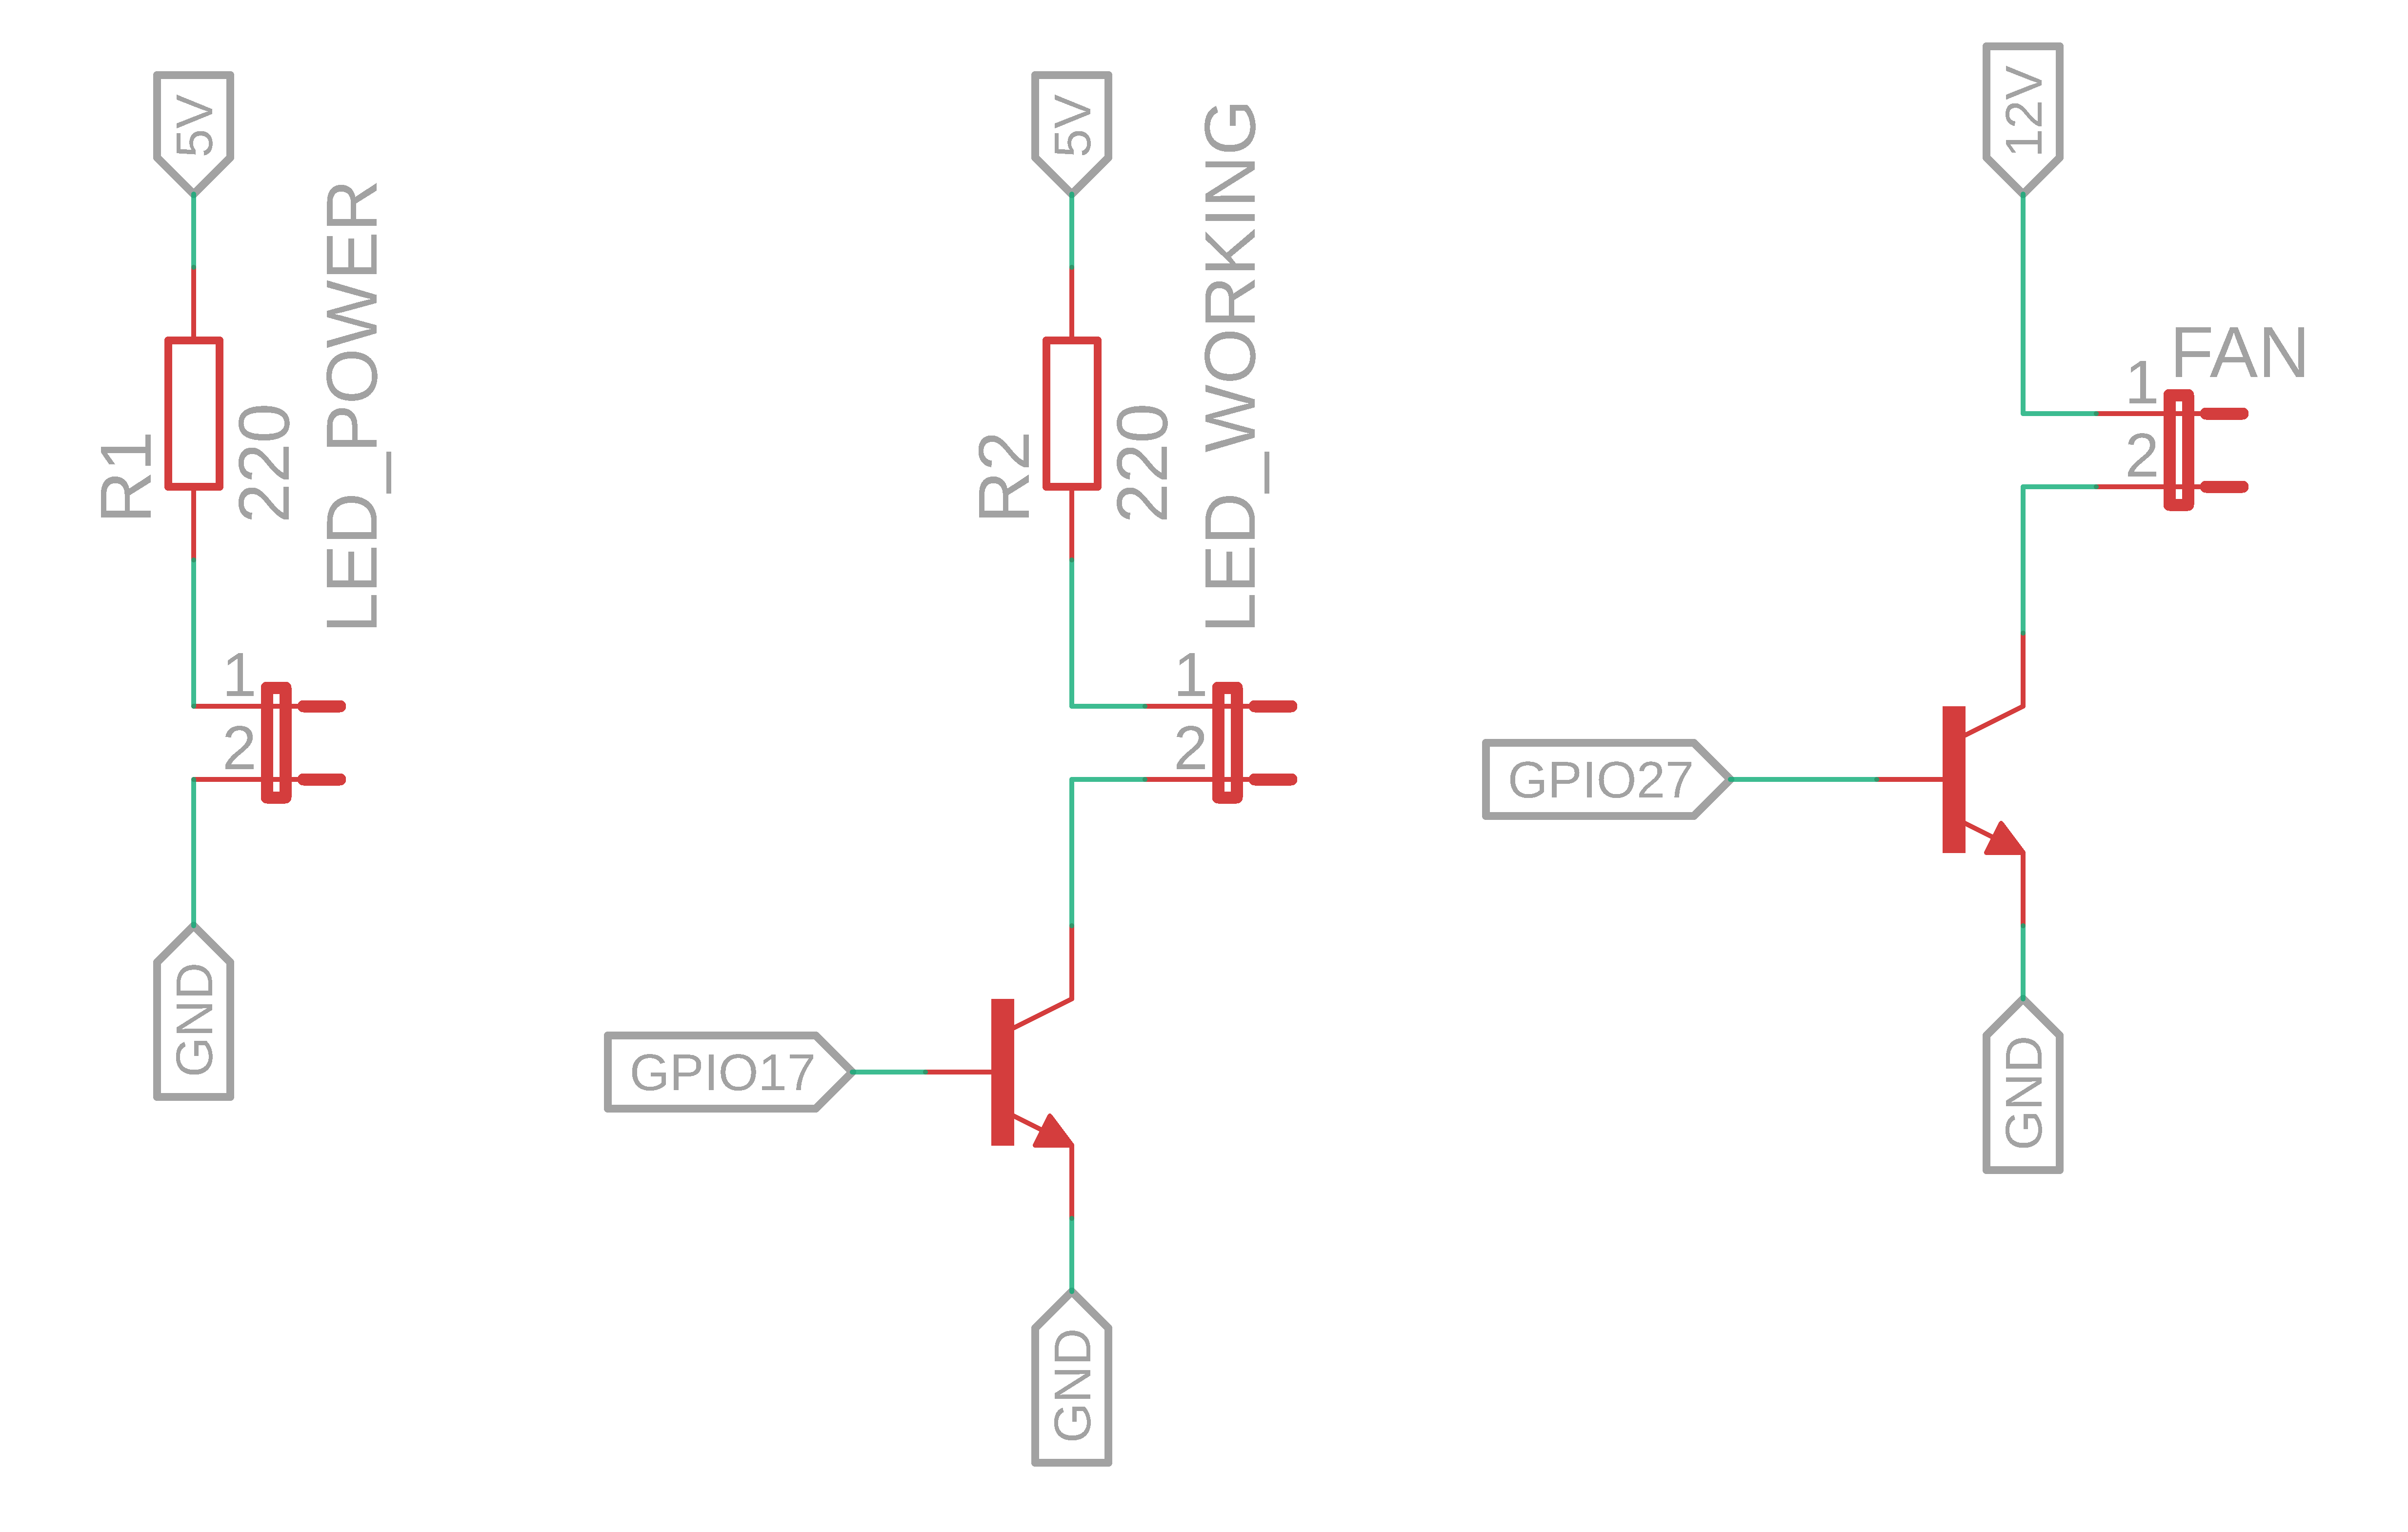
\includegraphics[width=0.6\textwidth]{images/Hardware/Schaltplan/Leds}
	\caption{Schaltplan: Leds und Kühler}
	\label{leds}
\end{figure}



\subsection{Layout}

Die in Kapitel \ref{sec:Schaltplan} gezeigten Schaltpläne werden in ''EAGLE'' zu einem Layout verarbeitet. Dabei wird vor allem auf eine praktische Anordnung der Komponenten und sinnvolle Leiterbahnführung geachtet.\\
Die Leiterbahnen für die 12 V Spannungsversorgung haben eine Breite von 1,78 mm. Die 5 V Leiterbahnen eine Breite von 1,27 mm. Für die restlichen Leiterbahnen reicht eine Breite von 0,82 mm. \\
Die roten Verbindungen in Abbildung \ref{layout} sind Verbindungen, die nach der Fertigung der Platine mit Drahtbrücken hergestellt werden müssen. \\
Die Platine hat eine Größe von 7,5 mm auf 10 mm und wird gefräst. Um die Übersichtlichkeit über die vielen Anschlussmöglichkeiten zu behalten, werden die jeweiligen Anschlüsse beschriftet. 


\begin{figure}[H]
	\centering
	\includegraphics[width=0.6\textwidth]{images/Hardware/Layout}
	\caption{Platinenlayout}
	\label{layout}
\end{figure}





 % Alexander
    %!TEX root = ../dokumentation.tex

\chapter{Code}
Die gewählte Sprache in welcher die Steuerung realisiert ist, ist Python. Python wurde gewählt, da mittels dieser die \acp{GPIO} des Raspberry Pi sehr einfach mittels einer Bibliothek ansteuerbar sind. Zudem ist Python eine sehr schnelle und weit verbreitete hochentwickelte Programmiersprache.\\
Bei der Erstellung des Codes, welcher das System steuert wurde von Anfang an eine Objektorientierte Vorgehensweiße gewählt, um eine möglichst Reibungslose und fortschrittliche Umsetzung zu realisieren.\\
Der gesamte Code wurde auf drei Dateien aufgeteilt, dies dient zum einen zur besseren Übersichtlichkeit, zum anderen erhielt jede Klasse eine eigene Datei.
\section{Motor}
Die erste Datei und Klasse beschäftigt sich mit der Ansteuerung der Schrittmotoren.\\
Sie benötigt zwei extra Bibliotheken (Listing \ref{motor_bib}). Die 'time' Bibliothek wird benötigt, um zwischen verschiedenen Befehlen 'schlafen' zu können, sprich das Programm pausieren zu können. Die 'RPI.GPIO' Bibliothek wird benötigt um die \acp{GPIO} des Raspberry PI ansteuern zu können. 
\begin{lstlisting}[caption={Bibliotheken der Motor Klasse}, language={Python}, label={motor_bib}, numbers=left]
import time
import RPi.GPIO as GPIO	
\end{lstlisting}

\subsection{Konstruktor} 
Der Konstruktor der Klasse beschäftigt sich mit der Deklaration von Variablen und dem zuweisen der dem Konstruktor übergebenen Parameter.\\
Im Falle der Motor Klasse bekommt der Konstruktor sechs Übergabeparameter, wovon allerdings ein Parameter ('self') eine Referenz auf das eigene Objekt ist.\\
Die restlichen übergebenen Parameter sind die \acp{GPIO}, welche für die Ansteuerung des Motortreibers benötigt werden.\\
Bei einem Blick auf den Code des Konstruktors (Listing \ref{motor_contructor}) sieht man die übernahme der Übergabeparameter in Klasseneigene Variablen (Zeile 2-6). Anschließend wird die Kommunikationsrichtung der \acp{GPIO} festgelegt (Zeile 7 - 11). In diesem Fall werden alle Pins als Ausgang benötigt.\\
Außerdem wird den \acp{GPIO} direkt ein Zustand zugewiesen (Zeile 12 - 16), in diesem Fall ist die Konfiguration so, dass der Motor Treiber mit Achtelschritten arbeitet und den Motor gegen den  Uhrzeigersinn drehen lässt.
\begin{lstlisting}[caption={Konstruktor der Motor Klasse}, language={Python}, label={motor_contructor}, numbers=left]
def __init__(self, Step, Dir, MS1, MS2, MS3):
    self.step = Step
    self.dir = Dir
    self.MS1 = MS1
    self.MS2 = MS2
    self.MS3 = MS3
    GPIO.setup(self.step, GPIO.OUT)
    GPIO.setup(self.dir, GPIO.OUT)
    GPIO.setup(self.MS1, GPIO.OUT)
    GPIO.setup(self.MS2, GPIO.OUT)
    GPIO.setup(self.MS3, GPIO.OUT)
    GPIO.output(self.step, GPIO.LOW)
    GPIO.output(self.dir, GPIO.LOW)
    GPIO.output(self.MS1, GPIO.HIGH)
    GPIO.output(self.MS2, GPIO.HIGH)
    GPIO.output(self.MS3, GPIO.LOW)
\end{lstlisting}

\subsection{Bewegen des Motors}
Die Motor Klasse besitzt zudem noch eine Funktion, mittels welcher sich der jeweilige Motor bewegen lässt (Listing \ref{motor_move}). In der Funktion wird zunächst die Drehrichtung je nach übergabeparameter gesetzt (Zeile 2 - 5), und anschließend ein bzw. je nachdem wie viele Schritte gefordert werden ausführt. Um einen kompletten Schritt zu vollenden, wird der dafür vorgesehene Pin des Motortreibers Ein und wieder Aus geschaltet. Die Zeit zwischen diesen beiden Vorgängen kann über einen Übergabeparameter der Funktion eingestellt werden (Zeile 8 - 13). Dies bestimmt direkt die Drehgeschwindigkeit des Motors. Wobei allerdings eine kleinere übergebene Zeit eine schnellere Drehung des Motors produziert. 
\begin{lstlisting}[caption={Funktion zum Bewegen des Motors}, language={Python}, label={motor_move}, numbers=left]
def moveMotor(self, dir, step, speed):
    if(dir):
        GPIO.output(self.dir, GPIO.HIGH)
    else:
        GPIO.output(self.dir, GPIO.LOW)

    i = 0
    while i < step:
        GPIO.output(self.step, GPIO.HIGH)
        time.sleep(speed)
        GPIO.output(self.step, GPIO.LOW)
        time.sleep(speed)
        i += 1
\end{lstlisting}


\section{Lidar}
Auch der \ac{LIDAR} Sensor hat eine eigene Datei sowie Klasse bekommen, dies soll dazu dienen, um mehrere verschiedene Sensoren konfigurieren zu können und diese dann schell und einfach mit denselben Funktionen auswählen zu können.\\
Die Klasse ist in ihrer jetzigen From bereits in der Lage zwei Verschiedene \ac{LIDAR} Sensoren zu bedienen.
Die Lidar Klasse benötigt zwei Bibliotheken (Listing \ref{lidar_bib}), mit der ersten kann eine Serielle Verbindung erstellt werden. Die Zweite Bibliothek wird benötigt, um einen der zwei Möglichen \ac{LIDAR} Sensoren anzusteuern \todo{Referenz VL53L1X}. 
\begin{lstlisting}[caption={Bibliotheken der Lidar Klasse}, language={Python}, label={lidar_bib}, numbers=left]
import serial
import VL53L1X
\end{lstlisting}

\subsection{Konstruktor und Variablen}
Die \ac{LIDAR} klasse besitzt zwei Variablen. Die Variable "dist" wird verwendet, um die gemessene Entfernung zu speichern und auf diese Zugreifen zu können.\\
Die zweite Variable wird als Flag bei Verwendung des \ac{LIDAR} Sensors 'TFMini' \todo{Referenz TFMINI} benötigt (Listing \ref{lidar_constructor}).\\
Der Konstruktor der Klasse ist zudem in der Lage je nachdem, welche Parameter angegeben werden, die korrekte Verbindung herzustellen. Je nachdem welche Werte angegeben und welche als "None"  definiert werden, stellt der Konstruktor entweder eine Verbindung über \ac{UART} (Zeile 9) oder \ac{I2C} (Zeile 11 - 13) her. 
\begin{lstlisting}[caption={Kostruktor der Lidar Klasse}, language={Python}, label={lidar_constructor}, numbers=left]
class LIDAR():
    dist = 0
    recievedData = False

    def __init__(self, uart, i2c):
        self.uart = uart
        self.i2c = i2c
        if(self.uart != None and self.i2c == None):
            self.ser = serial.Serial(self.uart, 115200, timeout=1)
        else:
            self.tof = VL53L1X.VL53L1X(i2c_bus=1, i2c_address=i2c)
            self.tof.open()
            self.tof.start_ranging(3)
\end{lstlisting}
\subsection{Aufnehmen von Messdaten}
Die Funktion um anschließend Daten vom \ac{LIDAR} Sensor zu bekommen ist auch in der Klasse definiert, somit kann für egal welchen Sensortyp über die selben Funktionsaufrufe die Distanz ermittelt werden. 
\begin{lstlisting}[caption={Funktion um Distanz vom \ac{LIDAR} Sensor zu erhalten}, language={Python}, label={lidar_getData}, numbers=left]
	def getData(self):
        if(self.uart != None and self.i2c == None):
            self.ser.reset_input_buffer()
            while(self.recievedData != True):
                while(self.ser.in_waiting <= 9):
                    if((b'Y' == self.ser.read()) and (b'Y' == self.ser.read())):
                        Dist_L = self.ser.read()
                        Dist_H = self.ser.read()
                        self.dist = (ord(Dist_H) * 256) + (ord(Dist_L))
                        for i in range (0,5):
                            self.ser.read()
                        self.recievedData = True
                        break
        else:
            self.dist = self.tof.get_distance() # Entfernung in mm
            self.dist = self.dist/10.0
\end{lstlisting}
In Listing \ref{lidar_getData} kann man sehen, dass ähnlich wie im Konstruktor je nachdem welcher Sensor 'ausgewählt' wurde unterschiedliche Methoden verwendet werden um Daten zu bekommen. Der erste Abschnitt in Zeile 3 - 13 ist für die Verwendung eines Sensors mittels \ac{UART} gedacht. Da \ac{UART} ein Serieller Bus ist, auf welchen vom Slave konstant Daten geschickt werden, wartet diese Funktion so lange, bis neue Daten ankommen. Die neuen Daten werden durch zwei aufeinander folgende 'Y' gekennzeichnet. Anschließend werden die Zwei bit für die Entfernung gespeichert (Zeile 7 \& 8) und zur Gesamtdistanz zusammengefügt (Zeile 9). Anschließend wird die bereits erwähnte Flag der Klasse gesetzt, damit nur ein einzelner Wert aufgenommen wird.\\
Die Zweite Methode in Zeile 15 - 16 ist deutlich einfacher, da hierbei eine Bibliothek verwendet werden kann und die Distanz lediglich in die richtige Größe konvertiert werden muss (Zeile 15 - 16).
\section{Steuerung}
Die dritte und letzte Datei beschäftigt sich mit der generellen Steuerung des Systems und dem Initialisieren und Aufrufen der Klassen und derer Funktionen.\\
Für die Steuerung des Systems werden einige Bibliotheken mehr benötigt.
\begin{lstlisting}[caption={Bibliotheken zur Steuerung des Systems}, language={Python}, label={main_bibliotheken}, numbers=left]
# Bibliotheken
import time
import datetime
import math
import RPi.GPIO as GPIO

# Eigene Dateien
import Lidar
import Motor

# GPIO Nummerierung gleich der Pin Nummer
GPIO.setmode(GPIO.BOARD)
GPIO.setwarnings(False)
\end{lstlisting}
Die Bibliotheken in Zeile 2 \& 3 (Listing \ref{main_bibliotheken})werden für die Benennung der Dateien, welche Produziert werden benötigt. Die 'math' Bibliothek wird für einige Berechnungen benötigt und die 'RPi.GPIO' wird wie bereits erwähnt benötigt und die \acp{GPIO} des Raspberry Pi möglichst einfach anzusteuern. Anschließend werden dann noch die zwei Klassen importiert welche in den vorangegangenen Abschnitten erklärt wurden. Zudem wird noch der Modus der \ac{GPIO} Nummerierung festgelegt. In diesem Fall ist der Modus gleich der Nummerierung der Pins auf dem Board. \todo{Bild GPIO pinout}\\
\subsection{Pin Definitionen und Initialisieren der Klassen}
Da wie in den Vorangegangenen Kapiteln erläutert wurde Klassen für Motor und Lidar erstellt wurden müssen diese nun auch aufgerufen und initialisiert werden. Zudem sind weitere \acp{GPIO} nötig um das gesamte System zu Steuern.
\begin{lstlisting}[caption={Initialisieren von Variablen und Klassen}, language={Python}, label={main_classes}, numbers=left]
# Pins & Definitionen
workingLED = 11
fan = 13
lightGate = 23 #SPI SCLK --> In Version 2 der Platine eigenen Pin zuweisen

# Motor 1, Nema 11
M1 = Motor.MOTOR(31,29,37,35,33)

# Motor 2, Nema 17
M2 = Motor.MOTOR(18,16,36,38,40)

# LIDAR Sensor
lidar = Lidar.LIDAR('/dev/ttyAMA0', none)
#lidar = Lidar.LIDAR(None, 0x29)
\end{lstlisting}
Zunächst werden die Pins für die verschiedenen auf der Platine vorgesehenen Funktionen definiert (Listing \ref{main_classes}). Eine Anmerkung hierzu ist, dass auf der Platine versäumt wurde einen Pin für die Lichtschranke zur Positionierung bereitzustellen, daher wurde hier der Pin verwendet, welcher eigentlich für den Seriellen Takt des \ac{SPI} zuständig ist. Außerdem wurden Pins für eine Status LED und einen Lüfter bereitgestellt. \\
Nach den normalen Pin Deklarationen werden die beiden Motoren durch die Klassen initialisiert. Dazu werden wie im Kapitel der Motorklasse beschrieben die Verschiedenen Pins zur Ansteuerung des Motortreibers dem Konstruktor der Klasse übergeben. Anschließend kann der Motor mittels den in der Klasse definierten Funktionen gesteuert werden.\\
Zuletzt muss nur noch der \ac{LIDAR} Sensor initialisiert werden, dazu kann wie in Zeile 13 \& 14 zu sehen ist eine der beiden Initialisierungsmöglichkeiten gewählt werden, um entweder einen Sensor mittels \ac{UART} oder \ac{I2C} zu verwenden.\\
\subsection{Zusätzliche Funktionen}
Nachdem alle benötigten Variablen für die \acp{GPIO} definiert sind, werden noch einige Funktionen benötigt um einen schöneren und übersichtlicheren Code zu erzeugen (Listing \ref{main_functions}). 
\begin{lstlisting}[caption={Funktionen für die Übersichtlichkeit des Codes}, language={Python}, label={main_functions}, numbers=left]
# Funktion um GPIO's zu Initalisieren
def initGPIO():
    GPIO.setup(workingLED, GPIO.OUT)
    GPIO.output(workingLED, GPIO.LOW)
    GPIO.setup(fan, GPIO.OUT)
    GPIO.output(fan, GPIO.LOW)
    GPIO.setup(lightGate, GPIO.IN)

def homeAxis():
    while(GPIO.input(lightGate)!=GPIO.HIGH):
        M2.moveMotor(1,1,0.001)
    count = 0
    while(GPIO.input(lightGate)==GPIO.HIGH):
        M2.moveMotor(1,1,0.001)
        count += 1
    M2.moveMotor(1,36,0.001)
\end{lstlisting}
Die erste Funktion (Zeile 2 - 7) dient dazu, um die übrigen \acp{GPIO} zu initialisieren und diesen einen Startwert zu geben. Hier werden die \acp{GPIO} welche für die LED und den Lüfter vorgesehen sind als Ausgang deklariert und als 'LOW' initialisiert. Der \ac{GPIO} Pin welcher für die Lichtschranke vorgesehen ist wird als Eingang deklariert.\\
Die zweite Funktion wird benötigt, um das System in horizontaler Richtung in die Ausgangslage zu bringen. Dazu wird der Motor 2, welcher für den Polarwinkel zuständig ist, so lange gedreht, bis dieser die Lichtschranke erreicht, und diese wieder verlässt. Da die Lichtschranke nicht zu 100\% am Kreisscheitelpunkt positioniert ist, wird nach verlassen der Lichtschranke mit einem Manuellen Kalibrationswert (Zeile 16) der Polarwinkel in Nulllage gebracht.\\
\subsection{Variablen deklaration und aufrufen von Funktionen}
Bevor mit dem eigentlichen Messen begonnen werden kann müssen noch einige Variablen definiert und Funktionen aufgerufen werden.
\begin{lstlisting}[caption={Aufrufen von Funktionen und Variablen deklaration}, language={Python}, label={main_setup}, numbers=left]
initGPIO()
lidar.getData()
lidar.recievedData = False
homeAxis()
time.sleep(2)

stepsFullRotM2 = 200*8*6
stepsQuartRotM1 = 50*4

M1dir = False
M2dir = True

lidar.getData()
print(lidar.dist)
lidar.recievedData = False

data = open("data_"+datetime.datetime.fromtimestamp(time.time()).strftime('%Y-%m-%d_%H-%M-%S')+".csv", "w")
data.write("Nr;Distance;Azimuth;Elevation\n")
valueNr = 1
\end{lstlisting}
In Zeile 1 (Listing \ref{main_setup}) werden zuerst die \acp{GPIO} initialisiert. Anschließend wird ein Wert vom \ac{LIDAR} ausgelesen  und die Flag des \acp{LIDAR} wieder auf 'False' gesetzt, damit dieser anschließend wieder Messwerte aufnehmen kann. Dies dient zum Funktionstest, bevor das System bewegt wurde. Wenn der Sensor beispielsweiße nicht korrekt verbunden wurde würde das System abbrechen bevor etwas Bewegt wurde. Danach wird das System in die Ausgangslage positioniert und eine kurze Zeit gewartet, bevor es mit dem eigentlichen Messvorgang losgeht.\\
Wie in Zeile 7 \& 8 zu sehen werden anschließend noch die Anzahl der benötigten Schritte für eine ganze Umdrehung und eine Viertelumdrehung berechnet. Diese Werte werden benötigt, um die grenzen für die Schleifen der Messung festzulegen. \todo{FEHLER?!} \\
In Zeile 10 \& 11 werden die Startrichtungen für die Motoren festgelegt.\\
Anschließend wird ein Messwert in die Konsole ausgegeben, um dem Bediener eine Rückmeldung zu geben, dass das System Ordnungsgemäß funktioniert.\\
\subsection{Erstellen der Datei zum Speichern der Daten}
Ein letzter Schritt ist noch nötig, bevor mit der Messung begonnen werden kann (Listing \ref{main_data}). Dabei wird die Datei in welcher die Messwerte abgespeichert werden erstellt. Die Datei wird dabei immer mit "data" und dem Aktuellen Datum sowie Timestamp versehen. Als letzte Aktion vor der Messung wird der Index des ersten Messwertes gleich 1 gesetzt.\\
\begin{lstlisting}[caption={Erstellen der Datei zum Speichern der Daten}, language={Python}, label={main_data}, numbers=left]
data = open("data_"+datetime.datetime.fromtimestamp(time.time()).strftime('%Y-%m-%d_%H-%M-%S')+".csv", "w")
data.write("Nr;Distance;Azimuth;Elevation\n")
valueNr = 1
\end{lstlisting}
Die \ac{csv} Datei in welcher die Daten gespeichert werden ist nach folgendem Schema aufgebaut:
\begin{table}[H]
	\centering
	\caption{Beispieldatei}
	\begin{tabular}{l|l|l|l}
		Nr & Distance & Azimuth & Elevation \\
		\hline
		1  & 105      & 0       & 0         \\
		2  & 105      & 0       & 0.18      \\
		3  & 106      & 0       & 0.36        
	\end{tabular}
\end{table}
Jeder Wert welcher in die Datei gespeichert wird bekommt einen Index, somit kann man einen Überblick behalten, wie viele Messwerte aufgezeichnet wurden. Die Zweite Spalte, welche in der Datei steht, ist für die Distanz vorgesehen, welche vom \ac{LIDAR} Sensor ermittelt wird. Die beiden letzten Spalten der dienen der Speicherung des Winkels welcher aus der Position der Schrittmotoren ermittelt wird. Die Distanz wird in $cm$ gespeichert und die beiden Winkel in Grad.
\todo{Tabelle bsp Daten}

\subsection{Schleifen der Steuerung}
\begin{lstlisting}[caption={Messen und Aufzeichnen der Entfernungen}, language={Python}, label={main_loop}, numbers=left]
countM1 = 0
countM2 = 0
while(countM1 < stepsQuartRotM1):
    if(M2dir):
        while(countM2 < stepsFullRotM2):
            lidar.getData()
            lidar.recievedData = False
            data.write(str(valueNr) + ";" + str(lidar.dist) + ";" + str(360.0*countM2/stepsFullRotM2) + ";" + str(90.0*countM1/stepsQuartRotM1) + "\n")
            M2.moveMotor(M2dir,4,0.00025)
            valueNr += 1
            countM2 += 4
    else:
        while(countM2 >= 0):
            lidar.getData()
            lidar.recievedData = False
            data.write(str(valueNr) + ";" + str(lidar.dist) + ";" + str(360.0*countM2/stepsFullRotM2) + ";" + str(90.0*countM1/stepsQuartRotM1) + "\n")
            M2.moveMotor(M2dir,4,0.00025)
            valueNr += 1
            countM2 -= 4
    M1.moveMotor(M1dir,4,0.0005)
    countM1 += 4
    M2dir = not M2dir

data.stop()
lidar.tof.stop_ranging()
\end{lstlisting}
Da in Python keine konventionellen 'for' Schleifen möglich sind, müssen 'while' Schleifen verwendet werden. Dazu wird eine extra Variable benötigt (Zeile 1 \& 2 Listing \ref{main_loop)}, um zu Überwachen wie oft die Schleife schon durchlaufen wurde. Da in diesem Fall zwei "while" Schleifen ineinander Verschachtelt wurden, werden auch zwei Variablen benötigt um die Anzahl der Durchläufe zu überwachen. \\
Die äußere Schleife wird nur so oft durchlaufen, bis der Motor 1, welcher für die Neigung des Polarwinkles zuständig ist, 90° erreicht. Im inneren dieser Schleife gibt es eine Besonderheit. Da sich die Kabel des oberen Aufbaus nur endlich oft Drehen können bis diese Verschleißen, muss das System nach jeden 360° die Richtung umkehren. Dafür werden 2 verschiedene Schleifen benötigt, da später der Winkel anhand des Counters der Schleifendurchläufe berechnet wird. Prinzipiell passiert in den Schleifen in Zeile 5 - 11 und Zeile 13 - 19 aber exakt das selbe. Zuerst werden neue Daten vom \ac{LIDAR} Sensor angefragt, und die Flag des Sensors gesetzt. Anschließend wird der ermittelte Wert zusammen mit den aktuellen Winkeln und einem Index in die '.csv' Datei gespeichert. Die Winkel werden dabei in Grad angegeben (Zeile 8 \& 16).\\
Nachdem die Werte gespeichert wurden, wird der Motor bewegt, in diesem Fall um vier schritte, was auch zeigt, dass das System in diesem Codebeispiel nur mit einem viertel der Auflösung in Horizontaler Richtung arbeitet. Anschließend wird der Index sowie der Schleifenzähler erhöht. Beim Schleifenzähler besteht der große Unterschied Zwischen den beiden 'while' Schleifen, da einmal die Schleife von 'vorne' und einmal von 'hinten' durchlaufen wird. Die Schrittweite vier ergibt sich aus der Anzahl der Schritte welche auch dem Motor übergeben wurden.\\
Wenn die innere Schleife eine volle 360° Drehung also eine komplette Rotation durchlaufen hat, wird der Motor 1, welcher für den Polarwinkel zuständig ist ebenfalls bewegt, in diesem Fall auch um vier Schritte was ein viertel der Vertikalen Auflösung bedeutet. Ebenfalls der zweite Schleifenzähler wird um vier erhöht, und die Richtung des Motors für die Horizontale Drehung wird umgekehrt, bevor die innere Schleife aufs neue durchlaufen wird.\\
Wenn die gesamte Messung abgeschlossen ist wird die Datei welche die Daten enthält geschlossen und die Messung gestoppt. Die Datei kann nun weiterverwendet und ausgewertet werden.
\todo{Hauptklasse}%Marcel
    %!TEX root = ../dokumentation.tex


\chapter{Auswertung und Darstellung mit Matlab}\label{chap:auswertung_matlab}

Die Daten werden nach Beendigung eines Scans exportiert und auf einem seperaten PC ausgewertet. Die Auswertung und Darstellung erfolgt mit Matlab. Matlab bietet sich an, da große Datenmengen schnell ausgewertet und dargestellt werden können. Zudem sind bereits Kenntnisse zum Importieren und Darstellen von .csv Dateien vorhanden. 

Die .csv Datei enthält die Rohdaten. Die Rohdaten bestehen pro Datenwert aus der Entfernung vom Messpunkt bis zum Hindernis in Metern. Zudem ist jedem Entfernungswert der Azimuth und die Elevation im Bezug zum jeweils gesetzten Nullpunkt zugeordnet. Die Messwerte sind fortlaufend nummeriert. 
Diese Werte müssen zuerst aus der .csv Datei in Matlab importiert werden. Anschließend erfolgt die Aufteilung des Datensatzen in die Vektoren Entfernung, Azimuth und Elevation.
Die beiden Winkelwerte zusammen mit dem Entfernungswert stellen Kugelkoordinaten dar. Diese müssen zur Darstellung in Matlab in kartesische Korrdinaten umgewandelt werden. 



\section{Importieren und Zuordnen der Messwerte}

Im ersten Teil des Auswertungs- und Darstellungsprogramms wird die .csv-Datei als gesamtes in Matlab importiert. Anschließend werden die einzelnen Spalten dementsprechenden Variablen zugeordnet, um die spätere Auswerung zu erleichtern.

Das Importieren der Daten erfolgt über die ''importdata'' Funktion von Matlab, die es ermöglicht, Datensätze aus einer seperaten Datei zu lesen. Das erste Argument der Funktion ist der relative Dateipfad zu der einzulesenden Datei. Dieser wird in Zeile 5 festgelegt. Das zweite Argument steht für das Trennzeichen, mit dem einzelne Elemente in Daten abgetrennt werden. Bei .csv-Dateien ist dies ein Semikolon. Der letzte Übergabeparameter gibt an, wie viele Kopfzeilen importiert werden sollen.

Die Importierte Daten liegen anschließend als Struct in der Variable "data" vor. Diese Struct enthält zum einen die Kopfzeile als Feld und zum andern die Messwerte ohne Kopfzeile. Für die weitere Verwendung der Daten, werden nur die Messwerte benötigt. Diese werden mit Zeile 8 extrahiert. 

Anschließend werden in Zeile 10 bis 12 die einzelnen Spalten separiert und einer passenden Variablen zugeordnet. 

\begin{lstlisting}[caption={Importieren und Zuordnen von .csv Dateien},language={Matlab}, label={import_data}, numbers=left]
% Anwendung zur Darstellung einer 3D Punktewolke aus einem LIDAR System
clear all;

% Importieren und Zuordnen der Messwerte
file = 'Messwerte-05-02/Aufloesung-hoch.csv';

data = importdata(file,';',1); 
data = data.data;

distance = data(:,2);
azimut = data(:,3);
elevation = data(:,4)
\end{lstlisting}


\section{Umwandlung von Kugelkoordinaten zu kartesischen Koordinaten}

Die Messpunkte liegen hardwarebedingt als Kugelkoordinaten vor. Dies bedeutet, dass jeder Punkt aus dem Abstand r zum Zentrum O, dem Polarwinkel $\theta$ und dem Azimutwinkel $\phi$ definiert wird.

Der Abstand r wird durch die Distanz des Punktes P von 0 bestimmt. Der Polarwinkel $\theta$ ist der Winkel zwischen Flächennormalen und dem Vektor OP. Das Gegenstück dazu ist die Höhe.  Der Polarwinkel reicht von 0 bis $\pi$. \\
Der Azimutwinkel ist der Winkel zwischen der x-Achse und der Projektion der Strecke OP auf die xy Ebene. Dieser Winkel reicht je nach Definition von  -$\pi$ bis $\pi$ oder von 0 bis 2$\pi$. Für das Lidar System wird die zweite Definition verwendet.

\begin{figure}[H]
	\centering
	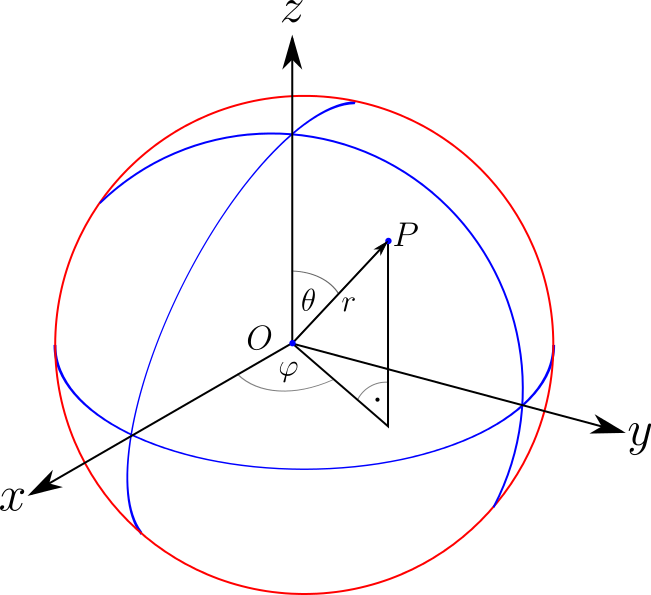
\includegraphics[width=0.75\textwidth]{images/Auswertung/Kugelkoordinaten}
	\caption{Kugelkoordinaten}
	\label{kugelkoordinaten}
\end{figure}



Da dass das Darstellen von Kugelkoordinaten in Matlab nicht ohne weiteres möglich ist, werden die Messwerte in kartesische Koordinaten umgerechnet.
Die Umrechnung erfolgt mit Formel \ref{umrechnung}:

\begin{equation}\formelentry{Umrechnung Kugelkoordinaten in kartesische Koordinaten}
\begin{split}
&x = r \cdot \cos(\theta) \cdot \cos(\phi) \\
&y = r \cdot \cos(\theta) \cdot \sin(\phi) \\
&z = r \cdot \sin(\theta)
\end{split}
\label{umrechnung}
\end{equation} 
\begin{flalign*}
&r = \text{Abstand des Punktes zum Zentrum} \left[m \right]&\\
&\theta = \text{Polarwinkel}\left[^{\circ} \right]&\\
&\phi = \text{Azimutwinkel}\left[^{\circ} \right]&
\end{flalign*}

In Matlab wird jeder einzelne Punkt innerhalb eine For-Schleife mit der oben genannten Formel umgewandelt und die drei Koordinaten x,y und z für kartesische Koordinaten gespeichert. Als Endwert der Schleife wird die Zeilenanzahl des Datensatzes verwendet. Somit ist dieser Wert variabel und muss nicht für jeden Datensatz spezifisch angepasst werden.\\
Die Berechnung befindet sich zudem in einer If-Abfrage, welche dazu dient, offensichtliche Messfehler zu entfernen. Alle Koordinaten, bei denen die Entfernung höher als 10 Meter ist, werden gelöscht. Die 10 Meter wurden auf experimenteller Basis und aufgrund der Größe des vorher definierten Standardraums festgelegt. Beim Lidar TF Mini werden nicht messbare Entfernungen mit einer Entfernung von 34999 Metern angegeben. Diese werden somit mit dieser Abfrage ebenfalls gefiltert.\\
Matlab rechnet bei trigonometrischer Funkionen mit dem Radiant. Die Winkel des Lidar Systems sind in Grad angegeben, weshalb sie innerhalb der Berechnung mit der Funktion deg2rad() in Radiant umgerechnet werden müssen.



\begin{lstlisting}[caption={Umwandlung von Kugelkoordinaten zu kartesischen Koordinaten},language={Matlab}, label={import_data}, numbers=left]
for i = 1:1:length(data)
	if(distance(i) < 1000)
		x(i) = -distance(i)*cos(deg2rad(elevation(i)))*cos(deg2rad(azimut(i)));
		y(i) = distance(i)*cos(deg2rad(elevation(i)))*sin(deg2rad(azimut(i)));
		z(i) = distance(i)*sin(deg2rad(elevation(i)));
	else
	end
end
\end{lstlisting}


\section{Darstellung der Messwerte}

Im letzten Teil des Programms werden die kartesischen Koordinatenpunkte in eine 3D-Darstellung umgewandelt. Zudem wird die Skalierung der Achsen festgelegt.


\begin{lstlisting}[caption={Darstellung der Messwerte},language={Matlab}, label={import_data}, numbers=left]
%plot3(x,y,z)			%Darstellung mit Linien
%plot3(x,y,z, '*')		%Darstellung mit Asteriskus 
plot3(x,y,z, '.')		%Darstellung mit kleinen Punkten
\end{lstlisting}

Die Darstellung der kartesischen Koordinaten erfolgt über die ''plot3()'' Funktion. Diese Funktion ermöglicht es, rotierbare, dreidimensionale Darstellungen anzufertigen. Die ersten drei Argumente der Funktion sind die Vektoren mit den jeweiligen Koordinaten.\\
Mit dem vierten Argument kann man die Darstellungsart der einzelnen Punkte festlegen. Anhand eines Datensatzes werden drei verschiedene Möglichkeiten auf Vor- und Nachteile überprüft.

Übergibt man der Funktion keinen Parameter, werden die Punkte durch schmale Linien verbunden. Dadurch entsteht ein dreidimensionaler Raum, mit sehr feiner Darstellung. Konturen sind dabei sehr gut zu erkennen. Zudem kann man den Verlauf der Messwertaufnahme erkennen. \\
Nachteil dieser Darstellungsart ist, dass auch Messfehler verbunden werden, wodurch es zu fehlerhaften Darstellungen kommt. Dies ist beispielsweise in Abbildung \ref{linien} zu erkennen.


\begin{figure}[H]
	\centering
	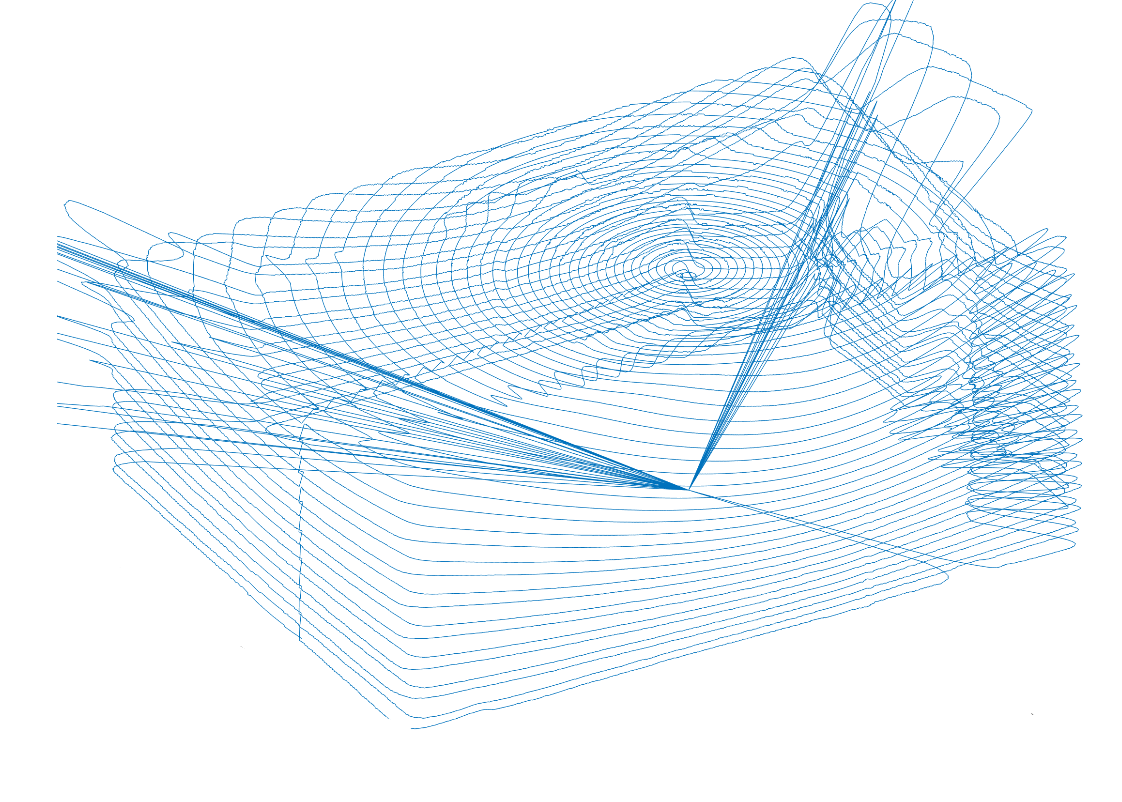
\includegraphics[width=0.7\textwidth]{images/Auswertung/Linien}
	\caption{Darstellung mit Linien}
	\label{linien}
\end{figure}

Einen weitere Möglichkeit der Darstellung sind Asterisken. Diese sind relativ zu den Linien sehr groß. Räume werden auch mit weniger Messpunkten erkennbar. Dadurch verschwimmen jedoch Aufnahmen mit höherer Auflösung und Details sind nicht mehr so gut erkennbar. 


\begin{figure}[H]
	\centering
	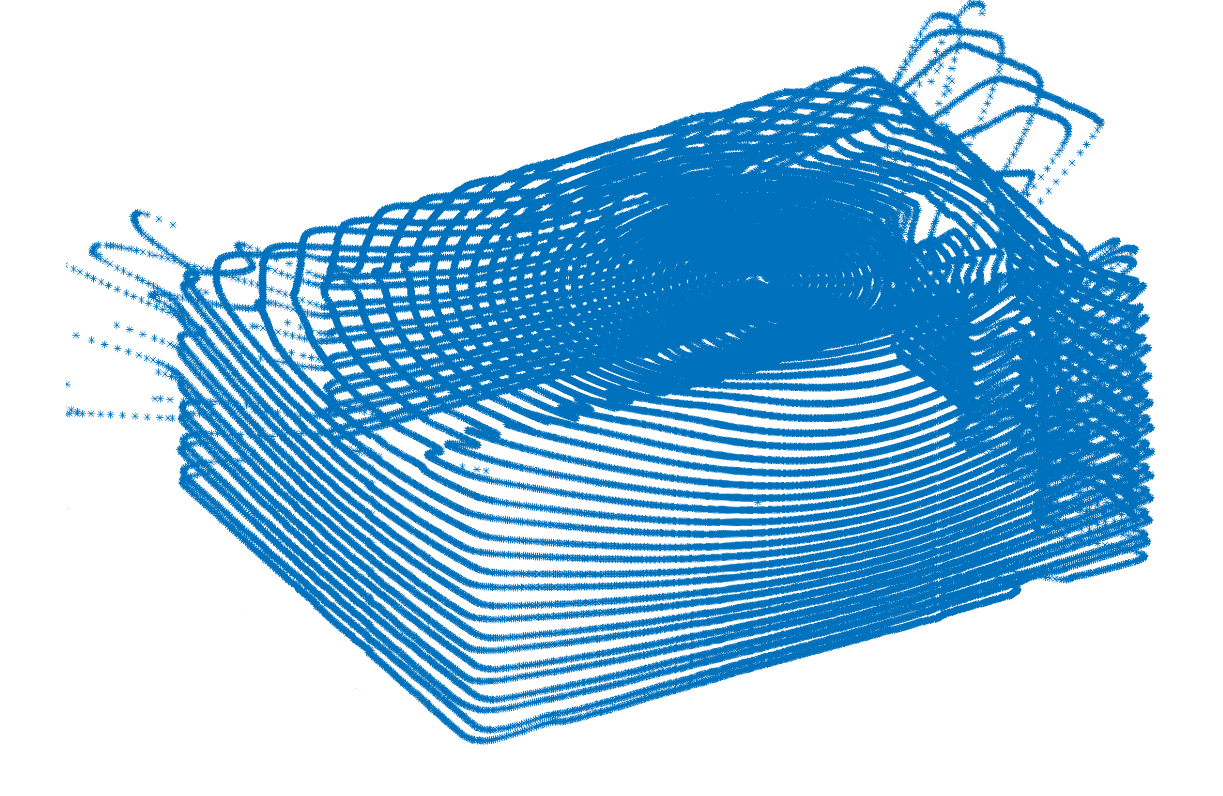
\includegraphics[width=0.7\textwidth]{images/Auswertung/Sternchen}
	\caption{Darstellung mit Asterisken}
	\label{asterisken}
\end{figure}

Die letzte Möglichkeit ist die Darstellung mit kleinen Koordinatenpunkten. Räume können bis ins sehr kleine Detail dargestellt werden und man hat trotz vieler Messpunkte und hoher Auflösung keine Stellen mit überladener Punkteanzahl. 



\begin{figure}[H]
	\centering
	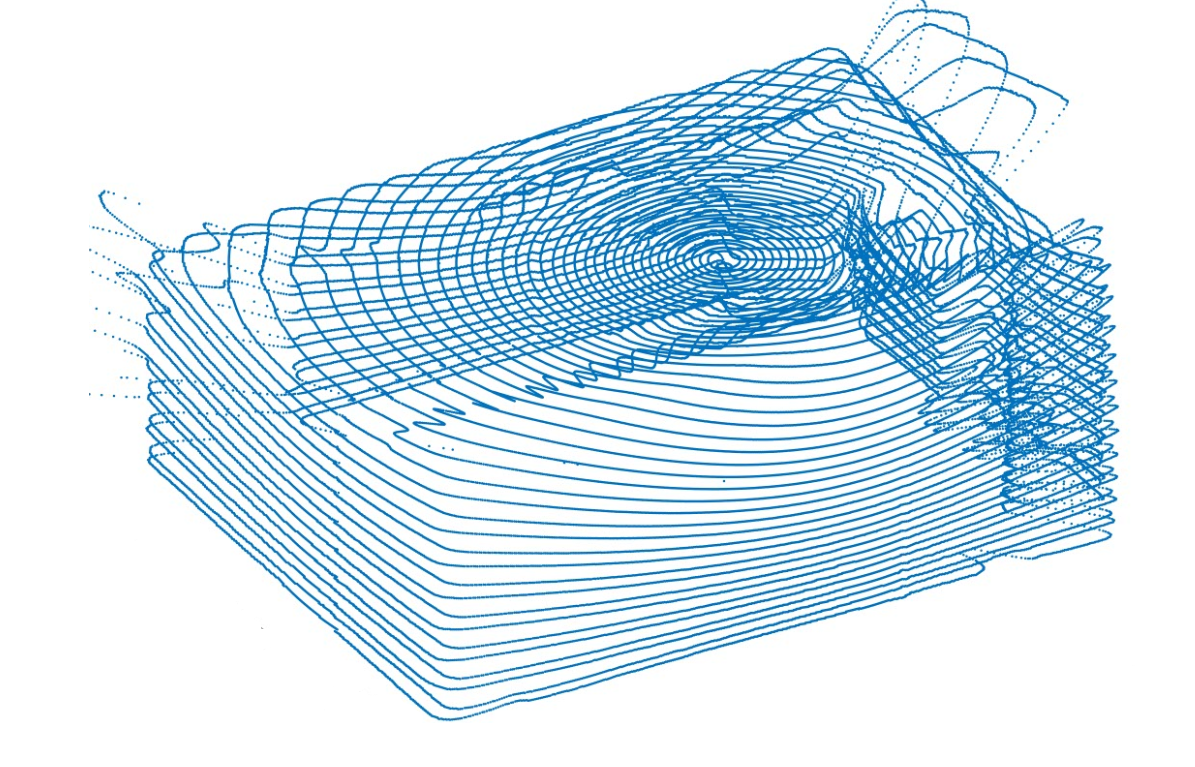
\includegraphics[width=0.7\textwidth]{images/Auswertung/Punkte}
	\caption{Darstellung mit Punkten}
	\label{punkte}
\end{figure}

Aufgrund der genannten Vor- und Nachteile wird in den meisten Fällen die Darstellung mit Punkten bevorzugt.  

Matlab skaliert die Achsen der Darstellung automatisch, weshalb teilweise schlecht auswertbare Bilder entstehen. Diese sind nur mit manueller Nachbearbeitung passend einstellbar. Um diese zusätzliche Arbeit zu automatisieren und die Darstellung einheitlich zu realisieren, werden die Achsen manuell mit der Funktion ''axis'' skaliert. Die ersten beiden Werte geben die Skala der x-Achse in Zentimetern an. Der zweite und dritte den Wert der y-Achse. Die letzten beiden Werte den Bereich der z-Achse.
Mit der Funktion ''pbaspect'' wird zudem die relative Größe der Achse in der späteren Darstellung festgelegt, um Verzerrungen zu vermeiden. 

\begin{lstlisting}[caption={Skalieren der Achsen},language={Matlab}, label={import_data}, numbers=left]
axis([-400 400 -400 400 0 240])
pbaspect([1 1 0.3])
\end{lstlisting}




%Alexander
    %!TEX root = ../dokumentation.tex


\chapter{Validierung des Systems}\label{chap:validierung}

Nachdem das Aufnehmen und Darstellen von Räumen funktioniert, wird die Genauigkeit des Systems untersucht. Zudem werden Versuche zu verschiedenen Auflösungen und unterschiedlichen Sensoren durchgeführt.  


\section{Genauigkeit des Systems}

Um die Genauigkeit des Systems zu überprüfen, wird ein Testraum mit dem Lidar-System vermessen. Im ersten Schritt wird das entstandene Modell grafisch mit einem manuell erstellten Modell verglichen.
Im Anschluss daran werden absolute Messwerte wie beispielsweise Raumhöhe, Länge und Breite verglichen.

	
\subsection{Grafischer Vergleich}

Beim grafischen Vergleich wird das von dem Lidar-System erstellte Modell mit einem manuell erstellten Modell grafisch verglichen.
Dazu wird der Testraum händisch vermessen und der Grundriss mit der Software ''Sweet Home 3D'' erstellt. \\
Bei dem Raum handelt es sich um einen Flur mit vielen Ecken, Türen und Gegenständen. Dadurch erhält man viele verschiedene Maße, die überprüft werden können. Der Grundriss des Raumes ist in Abbildung \ref{grundriss} dargestellt. 

\begin{figure}[H]
	\centering
	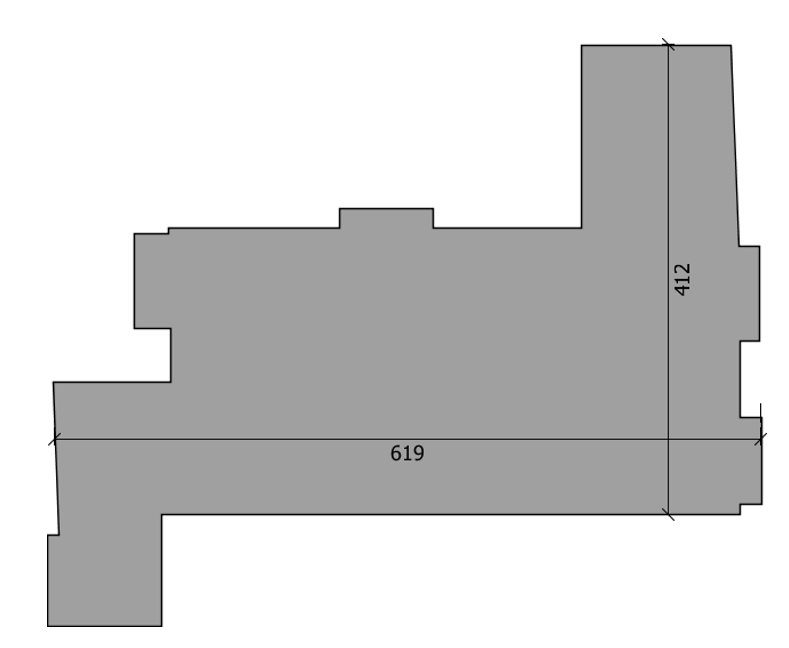
\includegraphics[width=0.6\textwidth]{images/Validierung/Grundriss}
	\caption{Grundriss des Testraums}
	\label{grundriss}
\end{figure}


Das Lidar-System wird im Raum aufgestellt. Die Position ist annähernd mittig und wird zudem bestimmt und in der Software eingetragen. Durch die Funktionsweise von Lidar Sensoren entstehen Schatten. So können beispielsweise Konturen hinter einer Wand, die die Lichtstrahlen reflektiert nicht detektiert werden. Diese Schatten werden ebenfalls im Grundriss eingezeichnet, um den Vergleich besser durchführen zu können. Die weißen Stellen innerhalb des Grundrisses in Abbildung \ref{grundrssmitschatte} stellen diese Schatten dar.

\begin{figure}[H]
	\centering
	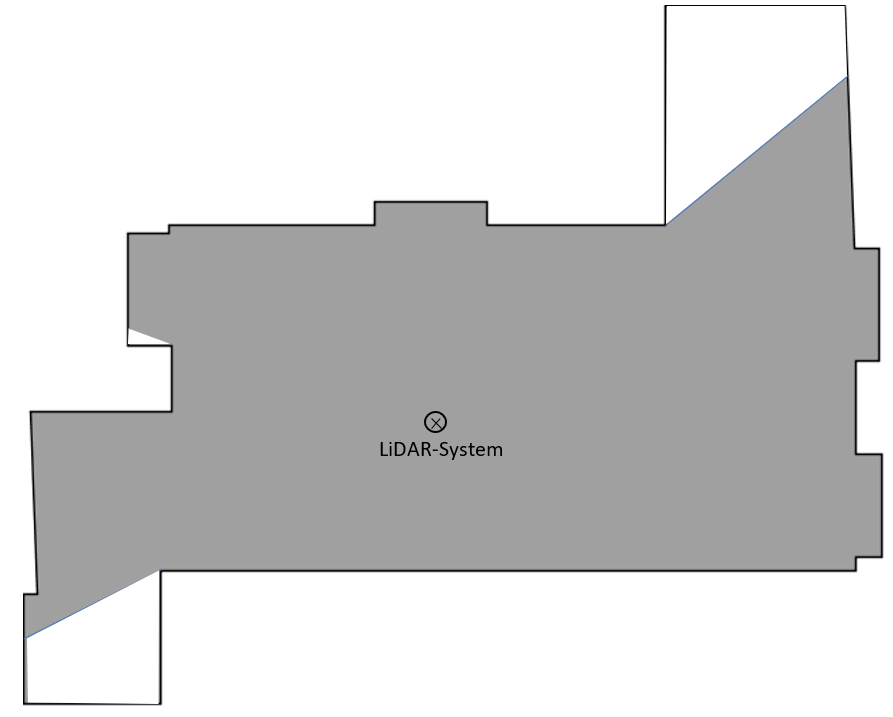
\includegraphics[width=0.7\textwidth]{images/Validierung/MitSchatten}
	\caption{Grundriss des Testraums}
	\label{grundrssmitschatte}
\end{figure}


Zum Vergleich wird nun der Grundriss benötigt, den das Lidar-System erstellt hat. Dazu wird die 3D Darstellung nur in z-Richtung betrachtet. Man erhält die Vogelperspektive des Raumes, bei dem der Grundriss auszumachen ist. 

\begin{figure}[H]
	\centering
	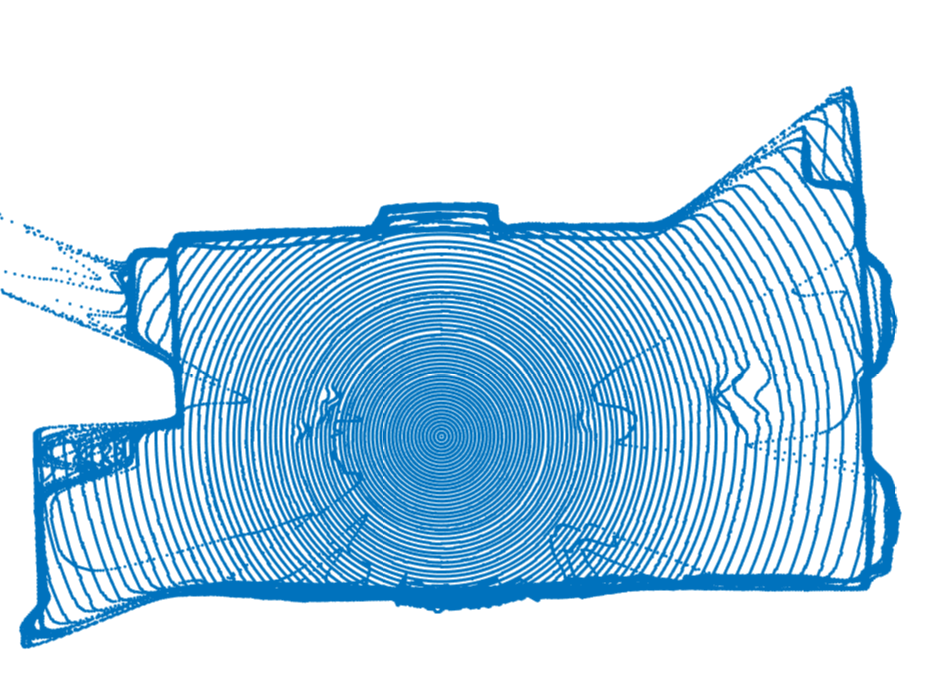
\includegraphics[width=0.7\textwidth]{images/Validierung/Vogelperspektive}
	\caption{Vogelperspektive des Testraums}
	\label{vogelperspektive}
\end{figure}


Zum grafischen Vergleich werden manuell erstellter Grundriss und die Vogelperspektive des Testraums mit einem Bildbearbeitungsprogramm im gleichen Maßstab übereinander gelegt.

\begin{figure}[H]
	\centering
	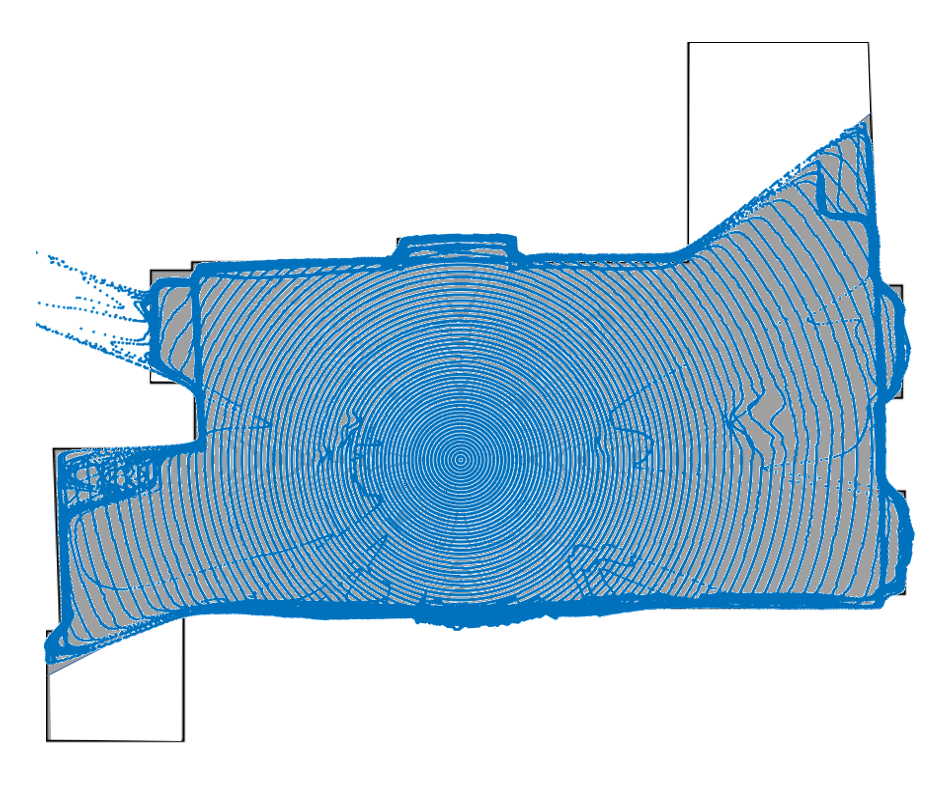
\includegraphics[width=0.7\textwidth]{images/Validierung/uebereinander}
	\caption{Grafischer Vergleich der Grundrisse}
	\label{uebereinander}
\end{figure}


Es ist zu erkennen, dass die beiden Grundrisse fast überall übereinstimmen. Auffällig sind die vielen Messwerte, die auf der linken Seite außerhalb des Raums liegen. An dieser Stelle befindet sich eine Glastüre. Diese wird von einem \ac{LIDAR} Sensor nicht detektiert, weswegen an dieser Stelle die Punkte abweichen. Zudem sind die Türrahmen auf der linken Seite nicht perfekt eckig, was auf weitere Schatten des Lasers schließen lässt.

Im 3D-Modell sind im Gegensatz zu dem Grundriss noch Möbel (links und rechts oben) zu erkenne. Zudem führen Lampen zu Unregelmäßigkeiten an der Decke.


\subsection{Vergleich absoluter Werte}

Es besteht die Möglichkeit, sich Koordinaten direkt in dem 3D-Modell mit sogenannten ''Data Cursors'' anzeigen zu lassen. Dadurch können absolute Distanzen abgelesen und mit dem Realwert verglichen werden.\\
In Abbildung \ref{messwerte} sind alle bis auf zwei Punkteebenen ausgeblendet. Es handelt sich um eine Draufsicht in z-Richtung. Mit Hilfe der eingetragenen Messpunkte können Distanzen im Raum bestimmt werden. Wie schon bei dem optischen Vergleich von realem Grundriss mit dem Modell kann so die Genauigkeit überprüft werden. Sowohl Länge als auch Breite des Modellraums stimmen bis auf geringe Abweichungen im Zentimeterbereich mit den realen Werten überein. Die Länge des Raumes ist im Modell 3,8 cm länger als in der Realität. Die Breite ist 1,8 cm geringer. Diese Abweichungen können sowohl auf Messabweichungen als auch auf die falsche Auswahl der Messpunkte zurückzuführen sein. \\
In Abbildung \ref{messwerte} ist zu erkennen, dass die Linien der Wände nicht an allen Stellen genau übereinander liegen. Vor allem auf der rechten Seite oberhalb des Messwertes ist dies zu sehen. An diesen Stellen liegen Messfehler des Systems vor. Die Streuung der Messwerte an einer geraden Wand wird in Abbildung \ref{wandbreite_alles} und \ref{wandbreite_label} detaillierter betrachtet.

\begin{figure}[H]
	\centering
	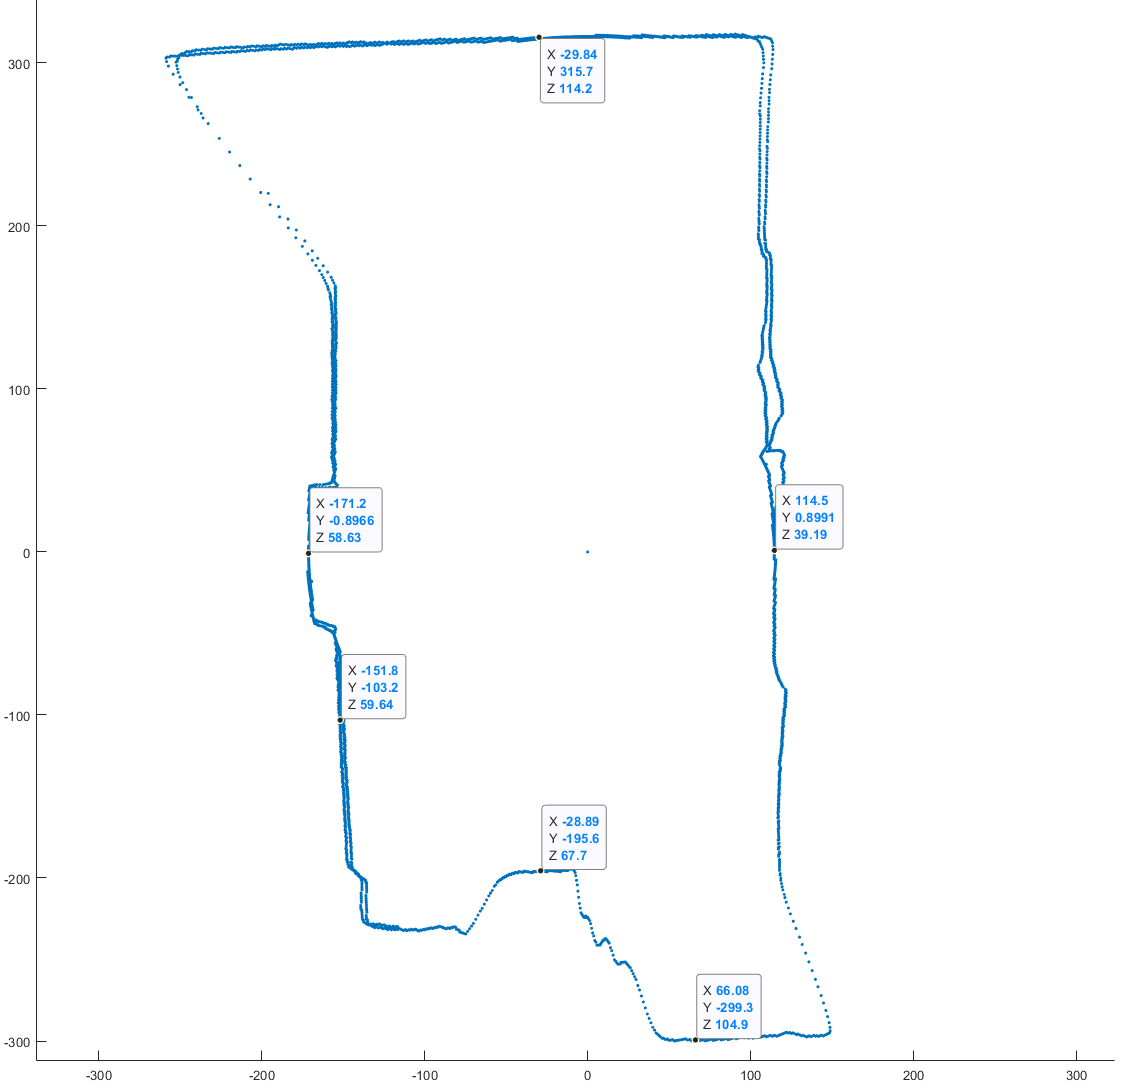
\includegraphics[width=0.6\textwidth]{images/Validierung/Genauigkeit/Messwerte.png}
	\caption{Messwerte über Data Coursor}
	\label{messwerte}
\end{figure}

Abbildung \ref{wandbreite_label} zeigt die Streuung der Messwerte an einer geraden Wand. Es handelt sich um eine Ansicht in z-Richtung. Dadurch betrachtet man die Wand von oben. Die verwendeten Messpunkte sind in Abbildung \ref{wandbreite_alles} in der Gesamtansicht des Modells eingezeichnet.  \\
Hätte das System keine Messabweichung, würden sich alle Punkte in Abbildung \ref{wandbreite_label} auf einer vertikalen Linie befinden. \\
Zur Bestimmung der Messabweichung werden zwei Messpunkte verwendet. Diese sind in x-Richtung möglichst weit voneinander entfernt. Die Distanz in x-Richtung entspricht der Streuung. Es kommt an dieser Stelle zu einer Streuung von 2,4 Zentimetern. Auffällig ist, dass je größer die Distanz der Messwerte in z-Richtung ist, desto größer wird die Distanz der Messpunkte in x-Richtung.\\
Das lässt darauf schließen, dass nicht der Sensor diese Messungenauigkeit hervorruft. Es ist möglich, dass Ungenauigkeiten bei der Kalibrierung des Sensors oder die Mechanik selbst diese Abweichungen hervorrufen. 


\begin{figure}[htb]
	\centering
	\begin{minipage}[t]{0.45\linewidth}
		\centering
		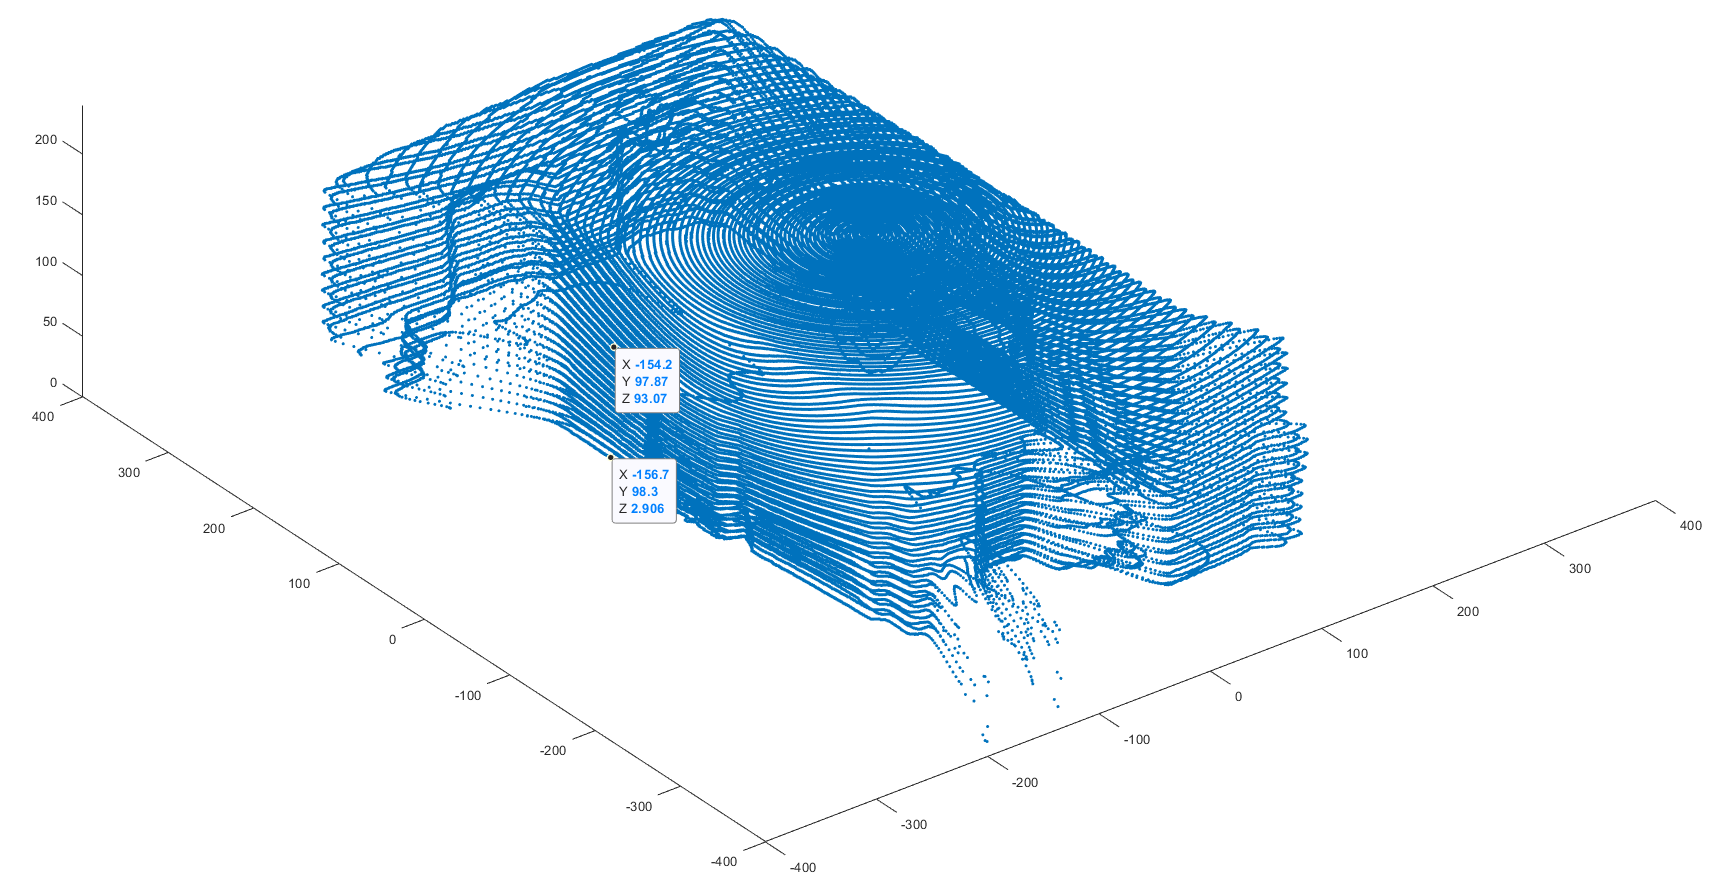
\includegraphics[width=1.2\linewidth]{images/Validierung/Genauigkeit/wandbreite_alles.png}
		\caption{Streuung der Messwerte an einer Ebene - Übersicht der Messpunkte}
		\label{wandbreite_alles}
	\end{minipage}
	\hfill
	\begin{minipage}[t]{0.45\linewidth}
		\centering
		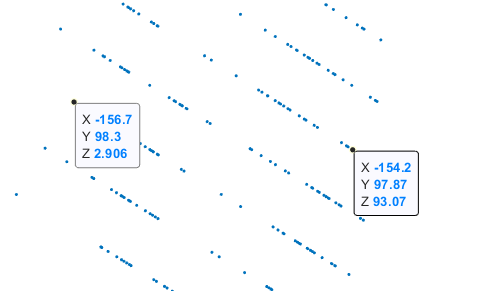
\includegraphics[width=1.2\linewidth]{images/Validierung/Genauigkeit/wandbreite.png}
		\caption{Streuung der Messwerte an einer Ebene}
		\label{wandbreite_label}
	\end{minipage}
\end{figure}


Eine weitere Größe, die zur Bestimmung der Genauigkeit des Systems überprüft wird, ist die Höhe des Raumes. Dazu wird von der Punktewolke wie in Abbildung \ref{Hoehe} zu sehen ist nur die xz-Ebene betrachtet. Zudem wird ein Messpunkt am oberen Rand, der die Decke des Testraums darstellt, eingefügt. Der z-Wert entspricht nun der Höhe des Raumes abzüglich der Höhe des Lidar-Systems. Dieser Wert entspricht in der Realität 175 cm. Das 3D Modell des Raumes zeigt einen z-Wert von 177,4 cm. Dies bedeutet, dass gemessener und realer Wert um 2,4 cm abweichen.
Diese Abweichung kann zum einen durch die Auswahl des Messpunktes kommen, da die Werte im z-Wert um wenige Zentimeter schwanken. Zum anderen ist eine Messungenauigkeit des Systems nicht auszuschließen.
 

\begin{figure} [H]
	\centering
	\includegraphics[width=0.7\textwidth]{images/Validierung/Genauigkeit/Hoehe1}
	\caption{Überprüfung der Höhe des Testraums}
	\label{Hoehe}
\end{figure}


\section{Vergleich verschiedener Auflösungen}

Durch das Einstellen verschiedener Schrittweiten der Schrittmotoren können unterschiedliche Auflösungen und Punkteverteilungen eingestellt werden. Derselbe Raum wird unter den gleichen Randbedingungen mit drei unterschiedlichen Einstellungen vermessen. Dabei bleibt sowohl die Position des \ac{LIDAR} Sensors als auch der Sensor selbst gleich. Verändert wird sowohl die horizontale als auch die vertikale Schrittweite. Dies kann im Code durch das Ändern weniger Parameter realisiert werden.

Bei den verschiedenen Auflösungen werden vor allem das Ergebnis und die benötigte Zeit zum Aufnehmen der Messdaten verglichen. Zudem soll dadurch eine Einstellung gefunden werden, die einen guten Kompromiss zwischen Auflösung und benötigter Zeit darstellt. 

Als Sensor wird der ''TF Mini Lidar'' verwendet.


\subsection{Übersicht über die Dauer, Auflösung und Anzahl an Messpunkten} \label{sec:auflösung}

Die horizontale Auflösung wird im Code in achtel Schritten des Schrittmotors angegeben. Der Motor läuft im Achtelschrittbetrieb. Für eine gesamte Umdrehung des Motors werden 200 Vollschritte benötigt. Zudem entspricht die Übersetzung von Schrittmotor zur drehbaren Basis des Lidar-Systems 1:6. Es werden also 9600 Achtelschritte benötigt, um die Basis einmal um 360 Grad zu drehen. Die Auflösung in Grad bezogen auf die Angabe im Code kann mit Formel \ref{horizontialeAuflösung} berechnet werden. 

\begin{equation}\formelentry{Berechnung horizontiale Auflösung}
d = \frac{360}{200 \cdot 8 \cdot 6} \cdot x
\label{horizontialeAuflösung}
\end{equation}
\begin{flalign*}
&x = \text{Anzahl Achtelschritte des Motors (in Software)} \left[^{\circ} \right]&\\
&d = \text{reale Drehung des Sensors in horizontaler Richtung}\left[^{\circ} \right]&\\
\end{flalign*}

Die vertikale Grundeinheit sind Viertelschritte. Um den Sensor um die maximalen 90 Grad drehen zu können, werden 50 Vollschritte benötigt. Der Sensor ist direkt mit der Welle des Motors verbunden, wodurch keine Konstante für eine Übersetzung benötigt wird.

\begin{equation}\formelentry{Berechnung vertikale Auflösung}
d = \frac{360}{50 \cdot 4} \cdot x
\label{vertikaleAuflösung}
\end{equation}
\begin{flalign*}
&x = \text{Anzahl Viertelschritte des Motors (in Software)} \left[^{\circ} \right]&\\
&d = \text{reale Drehung des Sensors in horizontaler Richtung}\left[^{\circ} \right]&\\
\end{flalign*}


Die Menge der Messpunkte lässt sich über die Anzahl der horizontalen Messpunkte multipliziert mit der Anzahl der vertikalen Reihen berechnen.

Die benötigte Zeit ist linear zu der Anzahl der Messpunkte.

\begin{table}
	\centering
	\caption{Übersicht verschiedene Auflösungen}	
		\begin{tabular} [H] {|c|c|c|c|}
		\hline
		\textbf{}										 &\textbf{Auflösung gering} & \textbf{Auflösung mittel}	& \textbf{Auflösung hoch} \\ \hline
		\begin{tabular}[x]{@{}c@{}}
			\textbf{Auflösung}\\\textbf{horizontial [$^{\circ} $]}
		\end{tabular}
			 & 1,2 	& 0,15 	 & 0,15			\\  \hline
		\begin{tabular}[x]{@{}c@{}}
			\textbf{Auflösung}\\\textbf{vertikal [$ ^{\circ} $]}
		\end{tabular}	 
			 & 14,4 & 7,2 	 & 3,6  		\\ \hline
		\begin{tabular}[x]{@{}c@{}}
			\textbf{Anzahl}\\\textbf{Messpunkte}
		\end{tabular}		 
			 & 7524 & 120049 & 240099 		\\ \hline
		\textbf{Dauer [min]}
			 & 2    & 31	 & 62 		 	\\ \hline
		
		\end {tabular}
		\label{uebersicht}
\end{table}


\subsection{Vergleich der unterschiedlichen Auflösungen}

Im Anschluss werden die 3D-Darstellungen grafisch verglichen und beurteilt.Vor allem die Darstellung von Details und die Richtigkeit der Maße wird überprüft. 

Um den Vergleich zu erleichtern, werden Bilder aus der jeweils gleichen Perspektive erstellt und verglichen. Der Maßstab ist bei jeder Darstellung identisch.
 
Die Aufnahme mit niedriger Auflösung besteht aus rund 7500 Bildpunkten. Die horizontale Auflösung ist mit 1,2 Grad Abstand zwischen zwei Punkten für nicht weit entfernte Gegenstände ausreichend. Bei größerer Entfernung wie z.B. in den Ecken des Raumes wird diese Auflösung an der Wand jedoch relativ schlecht und Details werden nicht mehr erkannt.
Die vertikale Auflösung von 14,4 Grad ist deutlich zu gering, um Details erkennen zu können. Türrahmen oder ähnliche größere Unebenheiten an der Wand sind nur grob auszumachen.   

\begin{figure}[H]
	\centering
	\includegraphics[width=0.9\textwidth]{images/Validierung/Aufloesungen/niedrig.png}
	\caption{Niedrige Auflösung}
	\label{niedrig}
\end{figure}


Bei der mittleren Auflösung werden etwa 16 mal so viele Bildpunkte aufgenommen wie bei der Messung mit geringer Auflösung. Die vertikale Schrittweite wird im Verglich zur ersten Messung halbiert, die horizontale beträgt mit 0,15 Grad ein Achtel der ursprünglichen Schrittweite. 

Die horizontalen Punkte verschmelzen zu einer Linie. Dies ist ein Zeichen dafür, dass die horizontale Auflösung von 0,15 Grad für den Testraum ausreichend ist. Durch die geringere vertikale Schrittweite erhält man doppelt so viele Messebenen. Dadurch werden Details wie beispielsweise Türrahmen, Lampen und weitere Gegenstände besser erkennbar. 


\begin{figure}[H]
	\centering
	\includegraphics[width=0.9\textwidth]{images/Validierung/Aufloesungen/mittel.png}
	\caption{Mittlere Auflösung}
	\label{mittel}
\end{figure}

Wie die Messung mit mittlerer Auflösung bereits gezeigt hat, reicht eine horizontale Schrittweite von 0,15 Grad bei der Größe des Testraums aus. Für den Test mit hoher Auflösung wird daher nur noch die vertikale Schrittweite halbiert. Dadurch verdoppelt sich die Anzahl der Bildpunkte. Die Messung benötigt jedoch ungefähr doppelt so lange.

Das Ergebnis ist eine 3D-Aufnahme, bei der sowohl horizontale als auch vertikale Auflösung gut ausreicht, um Details erkennen zu können.

\begin{figure}[H]
	\centering
	\includegraphics[width=0.9\textwidth]{images/Validierung/Aufloesungen/hoch.png}
	\caption{Hohe Auflösung}
	\label{hoch}
\end{figure}


Weiter werden die erstellten Grundrisse mit niedriger, mittlere und hoher Auflösung mit dem tatsächlichen Grundriss verglichen.

Der Vergleich zeigt, dass die Maße immer bis auf geringe Abweichungen mit dem tatsächlichen Grundriss übereinstimmten. Dabei macht die Auflösung keinen Unterschied. 

Deutlich erkennbar ist jedoch, wie in Abbildung \ref{vogel niedrigeAuflösung} zu sehen ist, dass bei niedriger Auflösung Details wie Türrahmen verschwimmen. Zudem sind die einzelnen Linienebenen leicht zueinander verschoben und nicht eindeutig zuordenbar.
Im Vergleich dazu sind bei der hohen Auslösung (Abbildung \ref{vogel hoheAuflösung}) klare Grundrisslinien erkennbar.

\begin{figure}[htb]
	\centering
	\begin{minipage}[t]{0.45\linewidth}
		\centering
		\includegraphics[width=1.2\linewidth]{images/Validierung/Aufloesungen/niedrig_vogel.png}
		\caption{Vogelperspektive niedrige Auflösung}
		\label{vogel niedrigeAuflösung}
	\end{minipage}
	\hfill
	\begin{minipage}[t]{0.45\linewidth}
		\centering
		\includegraphics[width=1.2\linewidth]{images/Validierung/Aufloesungen/hoch_vogel.png}
		\caption{Vogelperspektive hohe Auflösung}
		\label{vogel hoheAuflösung}
	\end{minipage}
\end{figure}


Im Großen und Ganzen lässt sich sagen, dass je nach Anforderung an das System die Parameter dementsprechend eingestellt werden müssen. Möchte man nur einen groben Überblick über den Raum, reicht ein schneller Scan mit niedriger Auflösung vollkommen aus. Möchte man hingegen eine detailreiche Darstellung, bei der man auch Details virtuell vermessen kann, wird eine hohe Auflösung benötigt. Dafür dauert solch eine Messung im Vergleich zur schnellen Messung recht lange.
Man sollte somit immer einen Kompromiss zwischen benötigter Auflösung und der Zeit für die Messung finden.

\section{Reale Auflösung im Testraum}

Im vorhergehenden Kapitel wurde die Auflösung über Winkelschritte direkt am Sensor bestimmt. In diesem Kapitel wird die reale Auflösung im Testraum überprüft. Dafür wird der absolute Abstand einzelner Messpunkte zueinander bestimmt. Um den Maximalwert der realen Auflösung in dem Testraum zu erhalten, wird das Modell aus Kapitel \ref{sec:auflösung} mit hoher Auflösung verwendet. Die horizontale Auflösung am Sensor beträgt 0,15 Grad. Die vertikale Schrittweite 3,6 Grad.\\
Als erster Messbereich wird die Wand mit der geringsten Distanz zum Sensor verwendet. In Abbildung \ref{realeAuslösung1_Übersicht} ist das gesamte Modell mit den in Abbildung \ref{realeAuslösung1} verwendeten Messpunkten zu sehen. Die horizontale Distanz der beider ausgewählter Messpunkte beträgt 0,442 cm. Die vertikale Distanz beträgt 3,61 cm. 

Rechnertisch beträgt die horizontale Distanz mit Formel \ref{realeAuflösung_formel} berechnet 0,4419 cm.

\begin{equation}\formelentry{Berechnung horizontale reale Auflösung}
d = tan(0,15) \cdot 168,8 \:cm 
\label{realeAuflösung_formel}
\end{equation}
\begin{flalign*}
&d = \text{Reale Distanz zweier Punkte in [cm]}&
\end{flalign*}

Dieser Wert ist allerdings nur eine Annäherung, da man mit der Formel davon ausgeht, dass die beiden Messpunkte mit dem Sensor ein rechtwinkliges Dreieck bilde. Zudem geht man davon aus, dass sich die beiden Messpunkte auf der gleichen z-Höhe wie der Sensor befinden.\\
Trotz dessen stimmen gerechneter und gemessener Wert sehr gut überein.   
\begin{figure}[H]
	\centering
	\begin{minipage}[t]{0.45\linewidth}
		\centering
		\includegraphics[width=1.2\linewidth]{images/Validierung/Aufloesungen/3Messwerte_Ansicht.png}
		\caption{Reale Auflösung im Testraum - geringe Entfernung - Übersicht}
		\label{realeAuslösung1_Übersicht}
	\end{minipage}
	\hfill
	\begin{minipage}[t]{0.45\linewidth}
		\centering
		\includegraphics[width=1.2\linewidth]{images/Validierung/Aufloesungen/3Label.png}
		\caption{Reale Auflösung im Testraum - geringe Entfernung}
		\label{realeAuslösung1}
	\end{minipage}
\end{figure}




Der zweite Testbereich befindet sich weiter entfernt vom Sensor. Dadurch wird die absolute Auflösung geringer.
Die horizontale Distanz der beider ausgewählter Messpunkte beträgt 0,79 cm. Die vertikale Distanz beträgt 5,12 cm.  

\begin{figure}[htb]
	\centering
	\begin{minipage}[t]{0.45\linewidth}
		\centering
		\includegraphics[width=1.2\linewidth]{images/Validierung/Aufloesungen/3Messwerte_Wand.png}
		\caption{Reale Auflösung im Testraum - große Entfernung - Übersicht}
		\label{realeAuslösung2_Übersicht}
	\end{minipage}
	\hfill
	\begin{minipage}[t]{0.45\linewidth}
		\centering
		\includegraphics[width=1.2\linewidth]{images/Validierung/Aufloesungen/Wand_3Messungen.png}
		\caption{Reale Auflösung im Testraum - große Entfernung}
		\label{realeAuslösung2}
	\end{minipage}
\end{figure}


Zudem kann man in Abbildung \ref{realeAuslösung2} sehen, dass die Messpunkte sehr gleichmäßig und symmetrisch über den Messbereich verteilt sind. 


\section{Vergleich der Sensoren}

Nachdem sowohl die Mechanik als auch der erste Lidar Sensor getestet und validiert wurden, soll ein kostengünstigerer Sensor getestet werden. Dazu werden zwei Aufnahmen mit den gleichen Einstellungen aber verschiedenen Sensoren aufgenommen. Die erste Messung wird mit dem Sensor "TF MINI" gemacht. Als zweiter Sensor wird der Sensor "VL53L1X" verwendet.

 

\begin{figure}[H]
	\centering
	\includegraphics[width=0.9\textwidth]{images/Validierung/Aufloesungen/mittel.png}
	\caption{Sensorvergleich: TF MINI}
	\label{hoch}
\end{figure}



\begin{figure}[H]
	\centering
	\includegraphics[width=0.9\textwidth]{images/Validierung/VL53.png}
	\caption{Sensorvergleich: VL53L1X}
	\label{vlx}
\end{figure}

Bei den Aufnahmen der Sensoren sind trotz selber Einstellungen sehr deutliche Unterschiede erkennbar. Während die Aufnahme mit dem ''TF MINI'' Sensor sehr deutliche Konturen erkennen lässt, verschwimmen diese bei dem zweiten Sensor. Es ist Auffallend, dass vor allem weiter entfernte Punkte nicht sauber aufgezeichnet werden können. So ist die Wand links oben beispielsweise nicht als solche zu erkenne. Die Punkte streuen zu sehr. Dies liegt vermutlich an der maximalen messbaren Distanz von 4 Metern bei optimalen Umgebungsbedingungen. Diese Bedingungen und Abhängigkeiten sind in Kapitel \ref{VL53L1X} genauer aufgeführt. Es kann davon ausgegangen werden, dass die Bedingungen bei der Messung nicht optimal waren und dewegen die maximal messbare Distanz kleiner war, als die Distaz, in der sich die Wand von dem Sensor befunden hat. 

Die folgenden beiden Abbildungen zeigen noch die jeweilige Vogelperspektive. \\



\begin{figure}[htb]
	\centering
	\begin{minipage}[t]{0.45\linewidth}
		\centering
		\includegraphics[width=1.2\linewidth]{images/Validierung/Aufloesungen/mittel_vogel.png}
		\caption{TF MINI - Vogelperspektive}
	\end{minipage}
	\hfill
	\begin{minipage}[t]{0.45\linewidth}
		\centering
		\includegraphics[width=1.2\linewidth]{images/Validierung/VL53_vogel.png}
		\caption{Sensor VL53L1X - Vogelperspektive}
	\end{minipage}
\end{figure}


Auch bei dieser Abbildung ist zu erkennen, dass der erste Sensor viel deutlichere Konturen abbildet und die Messungenauigkeit deutlich geringer ist. Sowohl nahe als auch weiter entfernte Wände werden zuverlässig erkannt. Beim zweiten Sensor wird wieder deutlich, dass alle Punkte, die etwas weiter vom Messpunkt entfernt sind, nur sehr ungenau oder gar nicht aufgenommen werden. 

Der Vergleich zeigt, dass der kostengünstigere Sensor ''VL53L1X'' unbrauchbar für das System ist. Die maximal messbare Distanz ist mit 4 Metern nur knapp über der Anforderung. Diese Distanz ist jedoch nur bei optimalen Umgebungsbedingungen realisierbar. Weichen diese Bedinungen beispielsweise durch schlecht Reflektierende Wände oder Umgebungslicht ab, sinkt die maximal messbare Distanz und die Messungenauigkeit steigt.  Dadurch entstehende fehlerhafte Abbildungen wie beispielsweise Abbildung \ref*{vlx}. Um dies zu verhindern, müssten die Umgebungsbedingungen dauerhaft angepasst und überwacht werden, was im Konflikt zu der Anforderung der Benutzerfreundlichkeit steht.\\

Der etwas teurere Sensor ''TF MINI'' hat in diesem Vergleich klar überzeugt. Unabhängig von Umgebungslicht, Reflexionseigenschaften der Wand und weiterer Parameter werden die Messwerte zuverlässig aufgenommen. 







%Alexander
    %!TEX root = ../dokumentation.tex
\chapter{Fazit}
\todo{Fazit}%
    %!TEX root = ../dokumentation.tex
\chapter{Ausblick}\label{chap:ausblick}
Im folgenden sollen Aspekte aufgeführt und erläutert werden, welche am \ac{LIDAR} System noch verbessert oder erweitert werden können. Teilweise sind für die Aspekte bereits Materialien vorhanden oder es wurden Verschiedene Methoden recherchiert. Alle unterlagen, welche mit dem Projekt verknüpft sind, sind im Github zu finden.\\
Die Verbesserungen werden in zwei Verschiedene Bereiche geteilt. Im Hardware Teil wird darauf eingegangen, welche Punkte an der Mechanik und/oder den Elektrischen Komponenten verbessert werden kann. Im zweiten Teil, der Software wird dann darauf eingegangen, wie man das System nutzerfreundlicher gestalten könnte.  
\section{Hardware}
\subsection{Platine}
Da beim Entwurf der Platine einige Fehler passiert sind, diese sind bereits im Layout behoben und die Platine muss neu gefräst werden. Bevor dies allerdings geschieht sollte diese auch neu gelayoutet werden, da es verschiedene Optimierungsmöglichkeiten gibt. \\
Die erste Optimierungsmöglichkeit für das neue Platinenlayout ist, dass ein Zusätzlicher Pin für die Lichtschranke heraus geführt wird, damit ist die Platine wieder so flexibel einsetzbar wie gedacht. Da dann auch ein Sensor welcher mittels \ac{SPI} angesteuert wird wieder einsetzbar ist.\\
Ein größerer Aspekt welcher im neuen Platinenlayout beachtet werden sollte ist, dass der Flachbandkabelstecker zum Raspberry Pi an den Rand zum Raspberry Pi hin umpositioniert wird. Dies erleichtert die Montage / Demontage der Platine oder des Raspberry Pi's. Zudem hat der Motortreiber des Motors 1 dann ausreichend Platz nach oben um entstehende Hitze abzuführen. Außerdem sind die gesamten Pins, welche vom Flachbandkabel verdeckt werden dann einfacher zu erreichen, dies bedeutet eine einfachere Wartung des \ac{LIDAR} Systems.
\subsection{Gyrosensor}
Im ursprünglichen Konzept des \ac{LIDAR} Systems war vorgesehen, dass sich sowohl die Horizontal- als auch die Vertikalachse selbstständig Kalibrieren können. Für die Horizontalachse hat dies durch die Verwendung einer Lichtschranke reibungslos geklappt, die Vertikalachse sollte sich mittels eines Gyrosensors in Nulllage, oder jede beliebige andere Lage, bringen können. Allerdings konnte dies im Rahmen der Studienarbeit nichtmehr implementiert werden, da der Sensor in ersten Tests zu ungenau war und weitere Tests nichtmehr möglich waren.. Der Sensor \todo{Name Sensor} ist bereits vorhanden und muss lediglich getestet und implementiert werden.
\subsection{Schleifring}
Ebenfalls war im Konzept und der \ac{CAD} Zeichnung des \ac{LIDAR} Systems die Verwendung eines Schleifrings geplant, da bei Verwendung kein umdrehen nach 360° nötig ist, sondern sich das System kontinuierlich in eine Richtung drehen kann.\\
Da es bei dem Schleifring allerdings zu Lieferschwierigkeiten kam, konnte dieser im Rahmen der Studienarbeit nicht verbaut werden. Die Bauteile sind allerdings so konstruiert, dass der vorgesehene Schleifring lediglich eingebaut werden müsste. 
\subsection{Motortreiber}
Der Motortreiber des Motors 1 also der vertikalen Achse sollte kontrolliert werden, da wie bereits erwähnt dieser bei korrekter Ansteuerung lediglich viertel Schritte tätigt. 
\subsection{Bedienfeld}
Ein weiterer Aspekt welcher bereits teilweise vorbereitet ist, ist die anbringung eines Bedienfelds an der front des \ac{LIDAR} Systems. Die bringt den Vorteil, dass die Messung nichtmehr über einen Computer gestartet werden muss, sondern das \ac{LIDAR} System alleinstehend verwendbar ist.\\
Mögliche Elemente, welche sowohl in Hard- als auch in Software erstellt werden müssen sind:
\begin{itemize}
	\item LCD Panel zur Ausgabe der Menüoptionen und des Fortschritts
	\item Drehencoder zur navigation im Menü
	\item Anbringen der Status LED's
	\item Anbringen des Ein- \& Ausschalters des \ac{LIDAR} Systems
\end{itemize}
Zum anbringen des Bedienfelds wurden bereits Nutensteine im vorderen Teil des Rahmens eingebracht, so dass man das Bedienfeld einfach anbringen kann.

\section{Software}
Damit einige der erwähnten Hardware Implementationen möglich sind müssen auch Anpassungen an der Software vorgenommen werden.
\subsection{Steuerung mit Übergabeparameter}
Um eine noch einfachere Steuerung des Systems zu ermöglichen können in Zukunft die Klassen so umgeschrieben werden, dass die Übergabe von Parametern möglich ist.\\
Eine möglicher aufruf eines Programms könnte dann wie folgt aussehen (Listing \ref{variables_calling}). Diese Funktion soll den Motor, welcher durch den ersten Übergabeparameter festgelegt wird um die Anzahl Schritte welche vom zweiten Übergabeparameter festgelegt werden drehen. Die Richtung soll dabei durch das Vorzeichen des zweiten Übergabeparameters bestimmt werden. Dabei soll ein positives Vorzeichen eine Drehung mit dem Uhrzeigersinn und ein negatives Vorzeichen eine Drehung gegen den Uhrzeigersinn bewirken.
\begin{lstlisting}[caption={Beispiel Aufruf einer Python Funktion mit Übergabeparametern}, language={bash}, label={variables_calling}, numbers=left]
python LIDAR_Bewegen.py 1 -400
\end{lstlisting}
Um diese Funktion zu implementieren müssen allerdings die Bestehenden Funktionen überarbeitet werden. In Listing \ref{variables_function} ist ein Code Beispiel für ein Programm welches über Übergabeparameter die Motoren steuern kann. Dieses Beispiel ist allerdings noch nicht am System selbst getestet worden. 
\begin{lstlisting}[caption={Python Beispiel Funktion welche Übergabeparamenter akzeptiert und ausführt}, language={python}, label={variables_function}, numbers=left]
## Programm zum Bewegen eines Motors

#Bibliotheken
import sys

#Eigene Dateien
import Motor


# Motor 1, Nema 11
M1 = Motor.MOTOR(31,29,37,35,33)

# Motor 2, Nema 17
M2 = Motor.MOTOR(18,16,36,38,40)

if(len(sys.argv) < 3):
    print("""Aufruf wie folgt:
    python LIDAR_Bewegen.py <nummerMotor> <Schritte>
    <nummerMotor> = 1 oder 2
    <Schritte> = positiv fuer Uhrzeigersinn, negativ fuer gegen den Uhrzeigersinn
    """)
else:
    m = sys.argv[1]
    s = sys.argv[2]
    dir = True
    if(s > 0):
        dir = True
    else if(s < 0):
        dir = False
        s = s * -1
    else:
        print("Bitte Schritte angeben")

    if(m == 1):
        M1.moveMotor(dir, s, 0.001)
    else if(m == 2):
        M2.moveMotor(dir, s, 0.001)
    else:
        print("Bitte Motor angeben")

\end{lstlisting}
Um die gewünschte Funktion zu implementieren ist die Bibliothek 'sys' sehr wichtig, denn diese Stellt die übergebenen Werte in einem Array zur Verfügung. Danach ist das Programm recht einfach aufgebaut, da in Zeile 7 - 14 die Motorklasse importiert und die beiden Motoren Initialisiert werden. Bevor mit dem eigentlichen ausführen des Programms, bzw. der Bewegung des Motors begonnen wird, wird überprüft ob mindestens 2 Werte übergeben wurden. Falls nicht wird eine Ausgabe darauf hinweißen und die Verwendung erläutern. \\
Anschließend wird ab Zeile 23 damit begonnen die übergebenen Werte in lokale Variablen zu übernehmen und die angegebene Richtung, welche beim Aufrufen durch das Vorzeichen des zweiten Parameters festgelegt wird, zu prüfen. Danach wird nur noch die Bekannte Funktion der Motor Klasse zum bewegen des Motors aufgerufen.

\subsection{Bedienfeld Statusausgabe und Steuerung}
Um ein Bedienfeld zu realisieren muss gegebenenfalls ein Komplettes Menü erstellt werden, durch welches die verschiedenen Funktionen aufrufbar sind. Bei der Implementierung gilt es darauf zu achten, dass die Objektorientierte Programmierung beibehalten wird und die Möglichkeit weitere Funktionen zu implementieren erhalten bleibt.\\
Um heraus zu finden wie weit eine Messung fortgeschritten ist, muss lediglich im Programmablauf beobachtet werden, wie viele der Festgelegten Messpunkte bereits aufgenommen wurden. Dies Kann relativ einfach über die beiden Zähler Variablen der while Schleifen realisiert werden. 
\todo{Recherche Python console Ladebalken und Pseudocode erstellen} 

\subsection{Webinterface}
Die selbe Steuerung welche über das Bedienfeld direkt am System möglich ist, kann auch am PC in einem ansprechenden \ac{GUI} möglich sein. Dazu ist die Idee, dies mittels einem Webinterface zu realisieren. Der Raspberry Pi könnte dazu ein eigenständiges \ac{WLAN} verwalten. Für die Darstellung der Website kann beispielsweiße ein NodeJS Server auf dem Raspberry Pi aufgesetzt werden. Um von javascript anfragen an den Server, bzw. Python zu senden kann die Bibliothek Flask verwendet werden. Im folgenden wird auf die Ideen zu den einzelnen Komponenten näher eingegangen. 
\subsubsection{\ac{WLAN} auf dem Raspberry Pi einrichten}
Da im Projekt ein Raspberry Pi der dritten Generation verwendet wurde, besitzt dieser durch den verbauten \ac{WLAN}-Chip die Möglichkeit ein eigenes \ac{WLAN}-Netzwerk zu erstellen und verwalten. https://www.raspberrypi.org/products/raspberry-pi-3-model-b/ 
Durch einige Änderungen in den Netzwerkeinstellungen lässt sich diese Funktion nutzen.
Zunächst müssen dafür die Packages zur Verwaltung der Zugriffe auf das Netzwerk installiert werden.
\begin{lstlisting}[caption={Installation dnsmasq hostapd}, language={bash}, numbers=left]
sudo apt-get install dnsmasq hostapd
\end{lstlisting}
Diese neu installierten Packages müssen anschließend auch konfiguriert werden. Dazu wird folgende Datei aufgerufen und durch eine Zeile ergänzt.
\begin{lstlisting}[caption={Konfiguration DHCP Server}, language={bash}, numbers=left]
Sudo nano /etc/dhcpcd.conf
\end{lstlisting}
Wird ergänzt durch
\begin{lstlisting}[caption={Konfiguration DHCP Server}, language={bash}, numbers=left]
Denyinterfaces wlan0
\end{lstlisting}
Damit der Raspberry Pi dann auch als Bereitsteller eines Netzwerks erkannt werden kann und immer wieder wird bekommt der Raspberry Pi eine Statische \ac{IP}-Adresse. 
\begin{lstlisting}[caption={Konfiguration Interfaces}, language={bash}, numbers=left]
Sudo nano /etc/network/interfaces
\end{lstlisting}
Wird dabei um mehrere Zeilen, welche zum Einstellen der Statischen \ac{IP}-Adresse dienen ergänzt.
\begin{lstlisting}[caption={Konfiguration Interfaces}, language={bash}, numbers=left]
allow-hotplug wlan0
iface wlan0 inet static
address 192.168.0.1
netmask 255.255.255.0
network 192.168.0.0
broadcast 192.168.0.255
\end{lstlisting}
Anschließend muss der dhcpcd client und der \ac{WLAN}-Chip neugestartet werden.
\begin{lstlisting}[caption={Konfiguration Interfaces}, language={bash}, numbers=left]
Sudo service dhcpcd restart
sudo ifdown wlan0; sudo ifup wlan0
\end{lstlisting}
Danach kann das Package, hostapt ebenfalls konfiguriert werden. 
\begin{lstlisting}[caption={Konfiguration Hostapd}, language={bash}, numbers=left]
Sudo nano /etc/hostapd/hostapd.conf
\end{lstlisting}
Dazu müssen folgende Zeilen in diese Datei geschrieben werden.
\begin{lstlisting}[caption={Konfiguration Hostapd}, language={bash}, numbers=left]
# Schnittstelle und Treiber
interface=wlan0
driver=nl80211
# WLAN-Konfiguration
ssid=LIDAR_WLAN
channel=1
hw_mode=g
ieee80211n=1
ieee80211d=1
country_code=DE
wmm_enabled=1
# WLAN-Verschluesselung
auth_algs=1
wpa=2
wpa_key_mgmt=WPA-PSK
rsn_pairwise=CCMP
wpa_passphrase=
\end{lstlisting}
Anschließend muss lediglich eine weitere Zeile ergänzt werden, damit die Konfiguration vollständig ist.
\begin{lstlisting}[caption={Konfiguration Hostapd}, language={bash}, numbers=left]
Sudo nano /etc/default/hostapd
\end{lstlisting}
Dort muss folgende Zeile ergänzt werden
\begin{lstlisting}[caption={Konfiguration Hostapd}, language={bash}, numbers=left]
DAEMON_CONF="/etc/hostapd/hostapd.conf"
\end{lstlisting}
Dann kann das letzte Package dnsmasq eingerichtet werden. Dieses Package ist dafür zuständig, die \ac{IP}-Adressen an die Nutzer des \ac{WLAN} zu verteilen.
Da die Grundkonfiguration von dnsmasq sehr viele Einstellungen beinhaltet sollte diese abgespeichert werden bevor eine neue eigene Konfigurationsdatei erstellt wird.
\begin{lstlisting}[caption={Konfiguration dnsmasq}, language={bash}, numbers=left]
sudo mv /etc/dnsmasq.conf /etc/dnsmasq.conf_alt
sudo nano /etc/dnsmasq.conf
\end{lstlisting}
Anschließend können folgende Zeilen in die neue Konfigurationsdatei eingetragen werden.
\begin{lstlisting}[caption={Konfiguration dnsmasq}, language={bash}, numbers=left]
Interface=wlan0
no-dhcp-interface=eth0
listen-address=192.168.0.1
bind-interfaces
server=8.8.8.8
dhcp-range=192.168.0.50,192.168.0.150,240h
\end{lstlisting}
Damit wenn der Raspberry Pi über \ac{LAN} an ein Netzwerk angeschlossen ist auch ein Internetzugriff stattfinden kann müssen die Pakete auch weitergeleitet werden, dazu sind weitere Einstellungen notwendig.
\begin{lstlisting}[caption={Konfiguration IPV4}, language={bash}, numbers=left]
Sudo nano /etc/sysctl.conf
\end{lstlisting}
Muss dazu mit der zeile
\begin{lstlisting}[caption={Konfiguration IPV4}, language={bash}, numbers=left]
Net.ipv4.ip_forward=1
\end{lstlisting}
Danach muss der Raspberry Pi Neu gestartet werden.
Anschließend müssen folgende Zeilen für die Weiterleitung Ausgeführt werden.
\begin{lstlisting}[caption={Konfiguration IPV4}, language={bash}, numbers=left]
sudo iptables -t nat -A POSTROUTING -o eth0 -j MASQUERADE
sudo iptables -A FORWARD -i eth0 -o wlan0 -m state -state RELATED,ESTABLISHED -j ACCEPT
sudo iptables -A FORWARD -i wlan0 -o eth0 -j ACCEPT
sudo sh -c "iptables-save > /etc/iptables.ipv4.nat"
\end{lstlisting}
Zuletzt muss noch eine Datei geändert werden.
\begin{lstlisting}[caption={Konfiguration IPV4}, language={bash}, numbers=left]
Sudo nano /etc/rc.local
\end{lstlisting}
Und folgende Zeile eingefügt werden
\begin{lstlisting}[caption={Konfiguration IPV4}, language={bash}, numbers=left]
Iptables-restore < /etc/iptables.ipv4.nat
\end{lstlisting}
Dann kann final der Hostapd und die dnsmasq gestartet werden.
\begin{lstlisting}[caption={Starten der neu installierten Packages}, language={bash}, numbers=left]
Sudo service hostapd start
sudo service dnsmasq start
Suod reboot
\end{lstlisting}
Nach dem Neustart des Raspberry Pi sollte ein \ac{WLAN} sichtbar sein um man sollte sich mit diesem Verbinden können. https://www.elektronik-kompendium.de/sites/raspberry-pi/2002171.htm https://www.randombrick.de/raspberry-pi-als-wlan-access-point-nutzen/ 


\subsubsection{NodeJS Server auf dem Raspberry Pi einrichten}
Um einen Webserver auf dem Raspberry Pi einrichten zu können wird NodeJS verwendet. Auch dies muss erst installiert und eingerichtet werden. 
\begin{lstlisting}[caption={Installation NodeJS}, language={bash}, numbers=left]
curl -sL https://deb.nodesource.com/setup_8.x | sudo -E bash -
sudo apt-get install -y nodejs
\end{lstlisting}
Ob die Installation erfolgreich war lässt sich mit folgendem Befehl überprüfen.
\begin{lstlisting}[caption={Installation NodeJS}, language={bash}, numbers=left]
node -v
\end{lstlisting}
%https://www.w3schools.com/nodejs/nodejs_raspberrypi.asp 

\subsubsection{Flask in Javascript und Python verwenden}
Flask ist ein Python Microframework, welches es ermöglicht verschiedene Routen direkt in Python über einen Webserver anzusprechen. Dies gibt in diesem Fall die Möglichkeit aus dem NodeJS Server heraus Python Programme zu starten. 
Um Flask zu verwenden muss dieses Natürlich zunächst Installiert werden. Dazu muss ein Ordner angelegt sein und in diesem Ordner eine Virtuelle Umgebung erstellt werden. 
\begin{lstlisting}[caption={Installation Flask}, language={bash}, numbers=left]
mkdir LIDAR
cd LIDAR
python3 -m venv venv
. venv/bin/activate
\end{lstlisting}
Anschließend kann Flask Installiert werden.
\begin{lstlisting}[caption={Installation Flask}, language={bash}, numbers=left]
Sudo pip install Flask
\end{lstlisting}
Nun kann eine Rote hinzugefügt werden, welche man dann, wenn der Flask Server gestartet ist über eine Route aufrufen kann. 
Im Fall dieses Projektes eignet sich Flask dazu die bereits vorhandenen Dateien aufrufen zu lassen. Die zugehörige Datei dazu könnte wie Folgt aussehen.
\begin{lstlisting}[caption={Flask Beispielprogram}, language={python}, numbers=left]
From flask import Flask
import subprocess
app=Flask(__name__)

@app.route('/movemotor1/<int: steps>')
def moveMotor1(steps):
	subprocess.run(["python", "LIDAR_Bewegen.py", "1", str(steps)])
	return;
@app.route('/movemotor2/<int: steps>')
def moveMotor2(steps):
	subprocess.run(["python", "LIDAR_Bewegen.py", "2", str(steps)])
	return;

\end{lstlisting}
Dies ist ein ungetesteter Beispielcode um die neu entworfene Funktion zum Bewegen der Motoren aufzurufen. Dabei ist es möglich über zwei verschiedene Routen die beiden Motoren anzusprechen und über einen Zusatz in der Route kann die Anzahl der Schritte angegeben werden. 
http://flask.pocoo.org 



%Marcel
    
    
    
    
    \label{endOfArabicNumbering}
    \clearpage

    \ifappendix
    % !TeX root = ../dokumentation.tex
\setpagestylefoot
\renewcommand{\thefigure}{A\arabic{figure}}
\renewcommand\thelstlisting{A\arabic{lstlisting}}
\renewcommand\thetable{A\arabic{table}}
\newcommand*{\fullref}[1]{\hyperref[{#1}]{\ref*{#1}. \nameref*{#1}}} 

% Nummer des Inhaltes mit \setcounter{figure}{"`Number"'} (figure, lstlisting or table) ändern wenn nötig

\addchap{\langanhang}


% Quellenverzeichnis nach Literatur und Weblinks trennen
%\printbibliography[heading=subbibintoc,title={Literatur},nottype=online]
%\printbibliography[heading=subbibintoc,title={Weblinks},type=online]

% Quellenverzeichnis nicht trennen
\ifliteratur
    \printbibliography[heading=subbibintoc]
\fi

% Glossar
\ifglossar
    \printglossary[style=altlist,title=\langglossar]
\fi

\newpage
\addsec{Aufteilung der Kapitel}
\begin{table}[H]
	\centering
	\caption{Aufteilung der Kapitel}
	\begin{tabular}{|l|l|}
		\hline
		\textbf{Kapitel} & \textbf{Author} \\\hline
		\fullref{chap:einleitung} & Alexander Kehrer \\\hline
		\fullref{sec:photodioden} & Marcel Wagner \\\hline
		\fullref{sec:schrittmotoren} & Alexander Kehrer \\\hline
		\fullref{chap:grund_lidar} & Marcel Wagner \\\hline
		\fullref{chap:stand_der_technik} & Marcel Wagner\\\hline
		\fullref{chap:machbarkeitsstudie} & Marcel Wagner \\\hline
		%\fullref{chap:matlab_modell} & Alexander Kehrer \\\hline
		\fullref{chap:mechanik} & Marcel Wagner \\\hline
		\fullref{chap:hardware} & Alexander Kehrer \\\hline
		\fullref{chap:code} & Marcel Wagner \\\hline
		\fullref{chap:auswertung_matlab} & Alexander Kehrer \\\hline
		\fullref{chap:validierung} & Alexander Kehrer \\\hline
		\fullref{chap:fazit} & Alexander Kehrer \\\hline
		\fullref{chap:ausblick} & Marcel Wagner \\\hline
	\end{tabular}
\end{table}

\newpage
\addsec{Github Repository}
Im Rahmen der Studienarbeit wurde ein Github Repository zur Verwaltung der Daten angelegt. Da die Dateien sehr umfangreich sind wird auf ein einzelnes einfügen verzichtet und stattdessen ein Verweis auf das Repository eingebracht.\\
Github Repository: \href{https://github.com/WagnerMarcel/LIDAR}{https://github.com/WagnerMarcel/LIDAR}
\begin{table}[H]
	\centering
	\caption{Verweise auf Github Repository}
	\begin{tabular}{|l|l|}
		\hline
		\textbf{Kapitel} & \textbf{Anhang} \\\hline
		\fullref{chap:einleitung} & - \\\hline
		\fullref{chap:grundlagen_et} & - \\\hline
		\fullref{chap:grund_lidar} & - \\\hline
		\fullref{chap:stand_der_technik} & -\\\hline
		\fullref{chap:machbarkeitsstudie} & \href{https://github.com/WagnerMarcel/LIDAR/tree/master/04_Protokolle}{Protokolle zu den Versuchen} \\\hline
		%\fullref{chap:matlab_modell} & \href{https://github.com/WagnerMarcel/LIDAR/tree/master/06_Matlab\%20Modell}{Matalb code zum Modell} \\\hline
		\fullref{chap:mechanik} & \href{https://github.com/WagnerMarcel/LIDAR/tree/master/08_Mechanik}{Technische Zeichnungen} \\\hline
		\fullref{chap:hardware} & \href{https://github.com/WagnerMarcel/LIDAR/tree/master/05_Datenblätter/VL53L1X}{Datenblätter} \& \href{https://github.com/WagnerMarcel/LIDAR/tree/master/09_Platinen}{Platinen}\\\hline
		\fullref{chap:code} & \href{https://github.com/WagnerMarcel/LIDAR/tree/master/07_Code}{Code} \\\hline
		\fullref{chap:auswertung_matlab} & \href{https://github.com/WagnerMarcel/LIDAR/tree/master/11_Auswertung}{Matlab Code \& Bilder} \\\hline
		\fullref{chap:validierung} & - \\\hline
		\fullref{chap:fazit} & - \\\hline
		\fullref{chap:ausblick} & - \\\hline
	\end{tabular}
\end{table}

\newpage
\addsec{Technische Zeichnungen}

\begin{figure}
	\includegraphics[width=\textwidth]{images/Mechanik/Grundflaeche}
	\caption{Grundfläche}
\end{figure}
\begin{figure}
	\includegraphics[width=\textwidth]{images/Mechanik/Seitenwand}
	\caption{Seitenwand}
\end{figure}

\begin{figure}
	\includegraphics[angle=90,origin=c, width=\textwidth]{images/Mechanik/Adapterplatte}
	\caption{Adapterplatte}
\end{figure}
\begin{figure}
	\includegraphics[angle=90,origin=c, width=\textwidth]{images/Mechanik/Basisplatte}
	\caption{Basisplatte}
\end{figure}



\begin{figure}
	\includegraphics[width=\textwidth]{images/Mechanik/Motoraufnahme}
	\caption{Motoraufnahme}
\end{figure}
\begin{figure}
	\includegraphics[angle=90,origin=c, width=\textwidth]{images/Mechanik/Rahmen}
	\caption{Rahmen}
\end{figure}



    \fi
\end{document}
